\documentclass[twoside]{book}

% Packages required by doxygen
\usepackage{fixltx2e}
\usepackage{calc}
\usepackage{doxygen}
\usepackage[export]{adjustbox} % also loads graphicx
\usepackage{graphicx}
\usepackage[utf8]{inputenc}
\usepackage{makeidx}
\usepackage{multicol}
\usepackage{multirow}
\PassOptionsToPackage{warn}{textcomp}
\usepackage{textcomp}
\usepackage[nointegrals]{wasysym}
\usepackage[table]{xcolor}

% Font selection
\usepackage[T1]{fontenc}
\usepackage[scaled=.90]{helvet}
\usepackage{courier}
\usepackage{amssymb}
\usepackage{sectsty}
\renewcommand{\familydefault}{\sfdefault}
\allsectionsfont{%
  \fontseries{bc}\selectfont%
  \color{darkgray}%
}
\renewcommand{\DoxyLabelFont}{%
  \fontseries{bc}\selectfont%
  \color{darkgray}%
}
\newcommand{\+}{\discretionary{\mbox{\scriptsize$\hookleftarrow$}}{}{}}

% Page & text layout
\usepackage{geometry}
\geometry{%
  a4paper,%
  top=2.5cm,%
  bottom=2.5cm,%
  left=2.5cm,%
  right=2.5cm%
}
\tolerance=750
\hfuzz=15pt
\hbadness=750
\setlength{\emergencystretch}{15pt}
\setlength{\parindent}{0cm}
\setlength{\parskip}{3ex plus 2ex minus 2ex}
\makeatletter
\renewcommand{\paragraph}{%
  \@startsection{paragraph}{4}{0ex}{-1.0ex}{1.0ex}{%
    \normalfont\normalsize\bfseries\SS@parafont%
  }%
}
\renewcommand{\subparagraph}{%
  \@startsection{subparagraph}{5}{0ex}{-1.0ex}{1.0ex}{%
    \normalfont\normalsize\bfseries\SS@subparafont%
  }%
}
\makeatother

% Headers & footers
\usepackage{fancyhdr}
\pagestyle{fancyplain}
\fancyhead[LE]{\fancyplain{}{\bfseries\thepage}}
\fancyhead[CE]{\fancyplain{}{}}
\fancyhead[RE]{\fancyplain{}{\bfseries\leftmark}}
\fancyhead[LO]{\fancyplain{}{\bfseries\rightmark}}
\fancyhead[CO]{\fancyplain{}{}}
\fancyhead[RO]{\fancyplain{}{\bfseries\thepage}}
\fancyfoot[LE]{\fancyplain{}{}}
\fancyfoot[CE]{\fancyplain{}{}}
\fancyfoot[RE]{\fancyplain{}{\bfseries\scriptsize Generated by Doxygen }}
\fancyfoot[LO]{\fancyplain{}{\bfseries\scriptsize Generated by Doxygen }}
\fancyfoot[CO]{\fancyplain{}{}}
\fancyfoot[RO]{\fancyplain{}{}}
\renewcommand{\footrulewidth}{0.4pt}
\renewcommand{\chaptermark}[1]{%
  \markboth{#1}{}%
}
\renewcommand{\sectionmark}[1]{%
  \markright{\thesection\ #1}%
}

% Indices & bibliography
\usepackage{natbib}
\usepackage[titles]{tocloft}
\setcounter{tocdepth}{3}
\setcounter{secnumdepth}{5}
\makeindex

% Custom commands
\newcommand{\clearemptydoublepage}{%
  \newpage{\pagestyle{empty}\cleardoublepage}%
}

\usepackage{caption}
\captionsetup{labelsep=space,justification=centering,font={bf},singlelinecheck=off,skip=4pt,position=top}

%===== C O N T E N T S =====

\begin{document}

% Titlepage & ToC
\pagenumbering{roman}
\begin{titlepage}
\vspace*{7cm}
\begin{center}%
{\Large L\+M\+PL \\[1ex]\large 1.\+0 }\\
\vspace*{1cm}
{\large Generated by Doxygen 1.8.11}\\
\end{center}
\end{titlepage}
\clearemptydoublepage
\tableofcontents
\clearemptydoublepage
\pagenumbering{arabic}

%--- Begin generated contents ---
\chapter{Todo List}
\label{todo}

\begin{DoxyRefList}
\item[\label{todo__todo000001}%
Class \doxyref{S\+B\+L\+Subdivision}{p.}{classSBLSubdivision} ]Do a defualt initialization of h. 
\end{DoxyRefList}
\chapter{Module Index}
\section{Modules}
Here is a list of all modules\+:\begin{DoxyCompactList}
\item \contentsline{section}{Motion\+Planning}{\pageref{group__MotionPlanning}}{}
\end{DoxyCompactList}

\chapter{Hierarchical Index}
\section{Class Hierarchy}
This inheritance list is sorted roughly, but not completely, alphabetically\+:\begin{DoxyCompactList}
\item Callback\begin{DoxyCompactList}
\item \contentsline{section}{Add\+Point\+Callback}{\pageref{structAddPointCallback}}{}
\item \contentsline{section}{Change\+Tree\+Callback}{\pageref{structChangeTreeCallback}}{}
\item \contentsline{section}{Closest\+Milestone\+Callback}{\pageref{structClosestMilestoneCallback}}{}
\item \contentsline{section}{Closest\+Milestone\+Callback}{\pageref{structClosestMilestoneCallback}}{}
\item \contentsline{section}{Pick\+Callback}{\pageref{structPickCallback}}{}
\item \contentsline{section}{Set\+Component\+Callback}{\pageref{structSetComponentCallback}}{}
\end{DoxyCompactList}
\item \contentsline{section}{C\+Space}{\pageref{classCSpace}}{}
\begin{DoxyCompactList}
\item \contentsline{section}{Explicit\+C\+Space}{\pageref{classExplicitCSpace}}{}
\begin{DoxyCompactList}
\item \contentsline{section}{Subgroup\+Explicit\+C\+Space}{\pageref{classSubgroupExplicitCSpace}}{}
\item \contentsline{section}{Subset\+Explicit\+C\+Space}{\pageref{classSubsetExplicitCSpace}}{}
\end{DoxyCompactList}
\item \contentsline{section}{Single\+Obstacle\+C\+Space}{\pageref{classSingleObstacleCSpace}}{}
\end{DoxyCompactList}
\item \contentsline{section}{Error\+Explaining\+Planner\+:\+:Edge}{\pageref{structErrorExplainingPlanner_1_1Edge}}{}
\item \contentsline{section}{S\+B\+L\+Tree\+:\+:Edge\+Info}{\pageref{structSBLTree_1_1EdgeInfo}}{}
\item \contentsline{section}{Edge\+Length\+Function}{\pageref{structEdgeLengthFunction}}{}
\item \contentsline{section}{Edge\+Planner}{\pageref{classEdgePlanner}}{}
\begin{DoxyCompactList}
\item \contentsline{section}{Bisection\+Epsilon\+Edge\+Planner}{\pageref{classBisectionEpsilonEdgePlanner}}{}
\item \contentsline{section}{Explicit\+Edge\+Planner}{\pageref{classExplicitEdgePlanner}}{}
\begin{DoxyCompactList}
\item \contentsline{section}{Bisection\+Epsilon\+Explicit\+Edge\+Planner}{\pageref{classBisectionEpsilonExplicitEdgePlanner}}{}
\end{DoxyCompactList}
\item \contentsline{section}{False\+Edge\+Planner}{\pageref{classFalseEdgePlanner}}{}
\item \contentsline{section}{Piggyback\+Edge\+Planner}{\pageref{classPiggybackEdgePlanner}}{}
\begin{DoxyCompactList}
\item \contentsline{section}{Edge\+Planner\+With\+C\+Space\+Container}{\pageref{classEdgePlannerWithCSpaceContainer}}{}
\end{DoxyCompactList}
\item \contentsline{section}{Straight\+Line\+Epsilon\+Planner}{\pageref{classStraightLineEpsilonPlanner}}{}
\item \contentsline{section}{Straight\+Line\+Obstacle\+Distance\+Planner}{\pageref{classStraightLineObstacleDistancePlanner}}{}
\item \contentsline{section}{True\+Edge\+Planner}{\pageref{classTrueEdgePlanner}}{}
\end{DoxyCompactList}
\item \contentsline{section}{Error\+Explaining\+Planner}{\pageref{classErrorExplainingPlanner}}{}
\item Generalized\+A\+Star\begin{DoxyCompactList}
\item \contentsline{section}{Greedy\+Subset\+A\+Star}{\pageref{structGreedySubsetAStar}}{}
\item \contentsline{section}{Optimal\+Subset\+A\+Star}{\pageref{structOptimalSubsetAStar}}{}
\end{DoxyCompactList}
\item \contentsline{section}{Incremental\+M\+M\+P\+R\+M\+\_\+\+Explicit}{\pageref{classIncrementalMMPRM__Explicit}}{}
\item \contentsline{section}{Incremental\+M\+M\+P\+R\+M\+\_\+\+Search}{\pageref{classIncrementalMMPRM__Search}}{}
\item \contentsline{section}{Int\+Triple}{\pageref{structIntTriple}}{}
\item \contentsline{section}{Less\+Edge\+Priority}{\pageref{structLessEdgePriority}}{}
\item \contentsline{section}{Tree\+Roadmap\+Planner\+:\+:Milestone}{\pageref{structTreeRoadmapPlanner_1_1Milestone}}{}
\item \contentsline{section}{Error\+Explaining\+Planner\+:\+:Milestone}{\pageref{structErrorExplainingPlanner_1_1Milestone}}{}
\item \contentsline{section}{Milestone\+Path}{\pageref{classMilestonePath}}{}
\item \contentsline{section}{Error\+Explaining\+Planner\+:\+:Mode}{\pageref{structErrorExplainingPlanner_1_1Mode}}{}
\item \contentsline{section}{Multi\+Modal\+P\+RM\+:\+:Mode\+Info}{\pageref{structMultiModalPRM_1_1ModeInfo}}{}
\item \contentsline{section}{Motion\+Planner\+Factory}{\pageref{classMotionPlannerFactory}}{}
\item \contentsline{section}{Motion\+Planner\+Interface}{\pageref{classMotionPlannerInterface}}{}
\begin{DoxyCompactList}
\item \contentsline{section}{Roadmap\+Planner\+Interface}{\pageref{classRoadmapPlannerInterface}}{}
\item \contentsline{section}{S\+B\+L\+Interface}{\pageref{classSBLInterface}}{}
\item \contentsline{section}{S\+B\+L\+P\+R\+T\+Interface}{\pageref{classSBLPRTInterface}}{}
\end{DoxyCompactList}
\item \contentsline{section}{Multi\+Modal\+C\+Space$<$ Mode $>$}{\pageref{classMultiModalCSpace}}{}
\item \contentsline{section}{Multi\+Modal\+C\+Space$<$ int $>$}{\pageref{classMultiModalCSpace}}{}
\begin{DoxyCompactList}
\item \contentsline{section}{Explicit\+M\+M\+C\+Space}{\pageref{classExplicitMMCSpace}}{}
\end{DoxyCompactList}
\item \contentsline{section}{Multi\+Modal\+P\+RM}{\pageref{classMultiModalPRM}}{}
\item \contentsline{section}{Path\+Info}{\pageref{structPathInfo}}{}
\item Path\+Int\+Callback\begin{DoxyCompactList}
\item \contentsline{section}{Connected\+Seed\+Callback}{\pageref{structConnectedSeedCallback}}{}
\item \contentsline{section}{Coverage\+Limited\+Path\+Callback}{\pageref{structCoverageLimitedPathCallback}}{}
\end{DoxyCompactList}
\item \contentsline{section}{Roadmap\+Planner}{\pageref{classRoadmapPlanner}}{}
\item \contentsline{section}{S\+B\+L\+Planner}{\pageref{classSBLPlanner}}{}
\begin{DoxyCompactList}
\item \contentsline{section}{S\+B\+L\+Planner\+With\+Grid}{\pageref{classSBLPlannerWithGrid}}{}
\end{DoxyCompactList}
\item \contentsline{section}{S\+B\+L\+P\+RT}{\pageref{classSBLPRT}}{}
\item \contentsline{section}{S\+B\+L\+Subdivision}{\pageref{classSBLSubdivision}}{}
\item \contentsline{section}{S\+B\+L\+Tree}{\pageref{classSBLTree}}{}
\begin{DoxyCompactList}
\item \contentsline{section}{S\+B\+L\+Tree\+With\+Grid}{\pageref{classSBLTreeWithGrid}}{}
\item \contentsline{section}{S\+B\+L\+Tree\+With\+Index}{\pageref{classSBLTreeWithIndex}}{}
\end{DoxyCompactList}
\item \contentsline{section}{Bisection\+Epsilon\+Edge\+Planner\+:\+:Segment}{\pageref{structBisectionEpsilonEdgePlanner_1_1Segment}}{}
\item Shortest\+Path\+Problem\begin{DoxyCompactList}
\item \contentsline{section}{Update\+Priority\+S\+PP}{\pageref{structUpdatePrioritySPP}}{}
\end{DoxyCompactList}
\item \contentsline{section}{Subset}{\pageref{structSubset}}{}
\item \contentsline{section}{Subset\+Cost}{\pageref{structSubsetCost}}{}
\item \contentsline{section}{Error\+Explaining\+Planner\+:\+:Transition}{\pageref{structErrorExplainingPlanner_1_1Transition}}{}
\item \contentsline{section}{Multi\+Modal\+P\+RM\+:\+:Transition\+Index}{\pageref{structMultiModalPRM_1_1TransitionIndex}}{}
\item \contentsline{section}{Multi\+Modal\+P\+RM\+:\+:Transition\+Info}{\pageref{structMultiModalPRM_1_1TransitionInfo}}{}
\item \contentsline{section}{Tree\+Roadmap\+Planner}{\pageref{classTreeRoadmapPlanner}}{}
\begin{DoxyCompactList}
\item \contentsline{section}{Perturbation\+Tree\+Planner}{\pageref{classPerturbationTreePlanner}}{}
\item \contentsline{section}{R\+R\+T\+Planner}{\pageref{classRRTPlanner}}{}
\begin{DoxyCompactList}
\item \contentsline{section}{Bidirectional\+R\+R\+T\+Planner}{\pageref{classBidirectionalRRTPlanner}}{}
\end{DoxyCompactList}
\end{DoxyCompactList}
\end{DoxyCompactList}

\chapter{Class Index}
\section{Class List}
Here are the classes, structs, unions and interfaces with brief descriptions\+:\begin{DoxyCompactList}
\item\contentsline{section}{{\bf Add\+Point\+Callback} }{\pageref{structAddPointCallback}}{}
\item\contentsline{section}{{\bf Bidirectional\+R\+R\+T\+Planner} \\*A single-\/query R\+RT (Rapidly-\/\+Exploring Random Tree) planner }{\pageref{classBidirectionalRRTPlanner}}{}
\item\contentsline{section}{{\bf Bisection\+Epsilon\+Edge\+Planner} }{\pageref{classBisectionEpsilonEdgePlanner}}{}
\item\contentsline{section}{{\bf Bisection\+Epsilon\+Explicit\+Edge\+Planner} }{\pageref{classBisectionEpsilonExplicitEdgePlanner}}{}
\item\contentsline{section}{{\bf Change\+Tree\+Callback} }{\pageref{structChangeTreeCallback}}{}
\item\contentsline{section}{{\bf Closest\+Milestone\+Callback} }{\pageref{structClosestMilestoneCallback}}{}
\item\contentsline{section}{{\bf Connected\+Seed\+Callback} }{\pageref{structConnectedSeedCallback}}{}
\item\contentsline{section}{{\bf Coverage\+Limited\+Path\+Callback} }{\pageref{structCoverageLimitedPathCallback}}{}
\item\contentsline{section}{{\bf C\+Space} \\*Motion planning configuration space base class }{\pageref{classCSpace}}{}
\item\contentsline{section}{{\bf Error\+Explaining\+Planner\+::\+Edge} }{\pageref{structErrorExplainingPlanner_1_1Edge}}{}
\item\contentsline{section}{{\bf S\+B\+L\+Tree\+::\+Edge\+Info} }{\pageref{structSBLTree_1_1EdgeInfo}}{}
\item\contentsline{section}{{\bf Edge\+Length\+Function} }{\pageref{structEdgeLengthFunction}}{}
\item\contentsline{section}{{\bf Edge\+Planner} \\*Abstract base class for an edge planner }{\pageref{classEdgePlanner}}{}
\item\contentsline{section}{{\bf Edge\+Planner\+With\+C\+Space\+Container} \\*Convenience class for edge planner that holds a smart pointer to a \doxyref{C\+Space}{p.}{classCSpace}. Typically used for single-\/obstacle edge checkers as follows\+: }{\pageref{classEdgePlannerWithCSpaceContainer}}{}
\item\contentsline{section}{{\bf Error\+Explaining\+Planner} \\*A planner that minimizes the the number of violated constraints using a R\+R\+T-\/like strategy }{\pageref{classErrorExplainingPlanner}}{}
\item\contentsline{section}{{\bf Explicit\+C\+Space} \\*Configuration space that exposes N obstacle checks. This functionality can be used in a motion planner to speed up planning by delaying certain expensive obstacle checks, or to provide reasons for infeasibility }{\pageref{classExplicitCSpace}}{}
\item\contentsline{section}{{\bf Explicit\+Edge\+Planner} \\*Default edge planner\+: checks each constraint sequentially using the space\textquotesingle{}s Local\+Planner(a,b,i) method }{\pageref{classExplicitEdgePlanner}}{}
\item\contentsline{section}{{\bf Explicit\+M\+M\+C\+Space} }{\pageref{classExplicitMMCSpace}}{}
\item\contentsline{section}{{\bf False\+Edge\+Planner} \\*Edge planner that is never visible }{\pageref{classFalseEdgePlanner}}{}
\item\contentsline{section}{{\bf Greedy\+Subset\+A\+Star} }{\pageref{structGreedySubsetAStar}}{}
\item\contentsline{section}{{\bf Incremental\+M\+M\+P\+R\+M\+\_\+\+Explicit} }{\pageref{classIncrementalMMPRM__Explicit}}{}
\item\contentsline{section}{{\bf Incremental\+M\+M\+P\+R\+M\+\_\+\+Search} }{\pageref{classIncrementalMMPRM__Search}}{}
\item\contentsline{section}{{\bf Int\+Triple} }{\pageref{structIntTriple}}{}
\item\contentsline{section}{{\bf Less\+Edge\+Priority} }{\pageref{structLessEdgePriority}}{}
\item\contentsline{section}{{\bf Tree\+Roadmap\+Planner\+::\+Milestone} }{\pageref{structTreeRoadmapPlanner_1_1Milestone}}{}
\item\contentsline{section}{{\bf Error\+Explaining\+Planner\+::\+Milestone} }{\pageref{structErrorExplainingPlanner_1_1Milestone}}{}
\item\contentsline{section}{{\bf Milestone\+Path} \\*A sequence of locally planned paths between milestones }{\pageref{classMilestonePath}}{}
\item\contentsline{section}{{\bf Error\+Explaining\+Planner\+::\+Mode} }{\pageref{structErrorExplainingPlanner_1_1Mode}}{}
\item\contentsline{section}{{\bf Multi\+Modal\+P\+R\+M\+::\+Mode\+Info} }{\pageref{structMultiModalPRM_1_1ModeInfo}}{}
\item\contentsline{section}{{\bf Motion\+Planner\+Factory} \\*A factory that assists with comparing the motion planners implemented in L\+M\+PL }{\pageref{classMotionPlannerFactory}}{}
\item\contentsline{section}{{\bf Motion\+Planner\+Interface} \\*A base class for a generic motion planner, which can be used to compare multiple planning algorithms under a common interface }{\pageref{classMotionPlannerInterface}}{}
\item\contentsline{section}{{\bf Multi\+Modal\+C\+Space$<$ Mode $>$} \\*Multi-\/modal configuration space base class }{\pageref{classMultiModalCSpace}}{}
\item\contentsline{section}{{\bf Multi\+Modal\+P\+RM} }{\pageref{classMultiModalPRM}}{}
\item\contentsline{section}{{\bf Optimal\+Subset\+A\+Star} }{\pageref{structOptimalSubsetAStar}}{}
\item\contentsline{section}{{\bf Path\+Info} }{\pageref{structPathInfo}}{}
\item\contentsline{section}{{\bf Perturbation\+Tree\+Planner} \\*A tree-\/based randomized planner that extends the roadmap by sampling the neighborhood of existing samples }{\pageref{classPerturbationTreePlanner}}{}
\item\contentsline{section}{{\bf Pick\+Callback} }{\pageref{structPickCallback}}{}
\item\contentsline{section}{{\bf Piggyback\+Edge\+Planner} }{\pageref{classPiggybackEdgePlanner}}{}
\item\contentsline{section}{{\bf Roadmap\+Planner} \\*A base roadmap planner class }{\pageref{classRoadmapPlanner}}{}
\item\contentsline{section}{{\bf Roadmap\+Planner\+Interface} }{\pageref{classRoadmapPlannerInterface}}{}
\item\contentsline{section}{{\bf R\+R\+T\+Planner} \\*A basic R\+RT (Rapidly-\/\+Exploring Random Tree) planner }{\pageref{classRRTPlanner}}{}
\item\contentsline{section}{{\bf S\+B\+L\+Interface} }{\pageref{classSBLInterface}}{}
\item\contentsline{section}{{\bf S\+B\+L\+Planner} \\*The S\+BL motion planner }{\pageref{classSBLPlanner}}{}
\item\contentsline{section}{{\bf S\+B\+L\+Planner\+With\+Grid} \\*An S\+BL planner whose trees use grids for point location }{\pageref{classSBLPlannerWithGrid}}{}
\item\contentsline{section}{{\bf S\+B\+L\+P\+RT} \\*A probabilistic roadmap of trees, where S\+BL is used for local planning }{\pageref{classSBLPRT}}{}
\item\contentsline{section}{{\bf S\+B\+L\+P\+R\+T\+Interface} }{\pageref{classSBLPRTInterface}}{}
\item\contentsline{section}{{\bf S\+B\+L\+Subdivision} \\*A grid-\/based subdivision to be used for S\+BL }{\pageref{classSBLSubdivision}}{}
\item\contentsline{section}{{\bf S\+B\+L\+Tree} \\*A tree of configurations to be used in the S\+BL motion planner }{\pageref{classSBLTree}}{}
\item\contentsline{section}{{\bf S\+B\+L\+Tree\+With\+Grid} \\*An S\+BL motion planner that uses a \doxyref{S\+B\+L\+Subdivision}{p.}{classSBLSubdivision} to pick the next node to expand, and nodes to connect }{\pageref{classSBLTreeWithGrid}}{}
\item\contentsline{section}{{\bf S\+B\+L\+Tree\+With\+Index} \\*An \doxyref{S\+B\+L\+Tree}{p.}{classSBLTree} with a node index }{\pageref{classSBLTreeWithIndex}}{}
\item\contentsline{section}{{\bf Bisection\+Epsilon\+Edge\+Planner\+::\+Segment} }{\pageref{structBisectionEpsilonEdgePlanner_1_1Segment}}{}
\item\contentsline{section}{{\bf Set\+Component\+Callback} }{\pageref{structSetComponentCallback}}{}
\item\contentsline{section}{{\bf Single\+Obstacle\+C\+Space} \\*Converges an \doxyref{Explicit\+C\+Space}{p.}{classExplicitCSpace} to a regular \doxyref{C\+Space}{p.}{classCSpace} based on one selected obstacle }{\pageref{classSingleObstacleCSpace}}{}
\item\contentsline{section}{{\bf Straight\+Line\+Epsilon\+Planner} \\*Straight-\/line edge planner that divides the segment until epsilon is reached }{\pageref{classStraightLineEpsilonPlanner}}{}
\item\contentsline{section}{{\bf Straight\+Line\+Obstacle\+Distance\+Planner} \\*Straight-\/line edge planner that divides the segment until the segment distance is below \doxyref{C\+Space.\+Obstacle\+Distance()}{p.}{classCSpace_a364b5b0ebcc258c39a263914ad3a0a89} }{\pageref{classStraightLineObstacleDistancePlanner}}{}
\item\contentsline{section}{{\bf Subgroup\+Explicit\+C\+Space} \\*Groups together multiple obstacles from an \doxyref{Explicit\+C\+Space}{p.}{classExplicitCSpace} }{\pageref{classSubgroupExplicitCSpace}}{}
\item\contentsline{section}{{\bf Subset} }{\pageref{structSubset}}{}
\item\contentsline{section}{{\bf Subset\+Cost} }{\pageref{structSubsetCost}}{}
\item\contentsline{section}{{\bf Subset\+Explicit\+C\+Space} \\*Extracts a subset of obstacles from an \doxyref{Explicit\+C\+Space}{p.}{classExplicitCSpace} }{\pageref{classSubsetExplicitCSpace}}{}
\item\contentsline{section}{{\bf Error\+Explaining\+Planner\+::\+Transition} }{\pageref{structErrorExplainingPlanner_1_1Transition}}{}
\item\contentsline{section}{{\bf Multi\+Modal\+P\+R\+M\+::\+Transition\+Index} }{\pageref{structMultiModalPRM_1_1TransitionIndex}}{}
\item\contentsline{section}{{\bf Multi\+Modal\+P\+R\+M\+::\+Transition\+Info} }{\pageref{structMultiModalPRM_1_1TransitionInfo}}{}
\item\contentsline{section}{{\bf Tree\+Roadmap\+Planner} \\*A base class to be used for tree-\/based roadmap planners }{\pageref{classTreeRoadmapPlanner}}{}
\item\contentsline{section}{{\bf True\+Edge\+Planner} \\*Edge planner that always is visible }{\pageref{classTrueEdgePlanner}}{}
\item\contentsline{section}{{\bf Update\+Priority\+S\+PP} }{\pageref{structUpdatePrioritySPP}}{}
\end{DoxyCompactList}

\chapter{Module Documentation}
\section{Motion\+Planning}
\label{group__MotionPlanning}\index{Motion\+Planning@{Motion\+Planning}}


Classes to assist in motion planning.  


\subsection*{Classes}
\begin{DoxyCompactItemize}
\item 
class {\bf Motion\+Planner\+Interface}
\begin{DoxyCompactList}\small\item\em A base class for a generic motion planner, which can be used to compare multiple planning algorithms under a common interface. \end{DoxyCompactList}\item 
class {\bf Motion\+Planner\+Factory}
\begin{DoxyCompactList}\small\item\em A factory that assists with comparing the motion planners implemented in L\+M\+PL. \end{DoxyCompactList}\item 
class {\bf C\+Space}
\begin{DoxyCompactList}\small\item\em Motion planning configuration space base class. \end{DoxyCompactList}\item 
class {\bf Edge\+Planner}
\begin{DoxyCompactList}\small\item\em Abstract base class for an edge planner. \end{DoxyCompactList}\item 
class {\bf Straight\+Line\+Epsilon\+Planner}
\begin{DoxyCompactList}\small\item\em Straight-\/line edge planner that divides the segment until epsilon is reached. \end{DoxyCompactList}\item 
class {\bf Straight\+Line\+Obstacle\+Distance\+Planner}
\begin{DoxyCompactList}\small\item\em Straight-\/line edge planner that divides the segment until the segment distance is below \doxyref{C\+Space.\+Obstacle\+Distance()}{p.}{classCSpace_a364b5b0ebcc258c39a263914ad3a0a89} \end{DoxyCompactList}\item 
class {\bf Bisection\+Epsilon\+Edge\+Planner}
\item 
class {\bf Explicit\+C\+Space}
\begin{DoxyCompactList}\small\item\em Configuration space that exposes N obstacle checks. This functionality can be used in a motion planner to speed up planning by delaying certain expensive obstacle checks, or to provide reasons for infeasibility. \end{DoxyCompactList}\item 
class {\bf Milestone\+Path}
\begin{DoxyCompactList}\small\item\em A sequence of locally planned paths between milestones. \end{DoxyCompactList}\item 
class {\bf Roadmap\+Planner}
\begin{DoxyCompactList}\small\item\em A base roadmap planner class. \end{DoxyCompactList}\item 
class {\bf Tree\+Roadmap\+Planner}
\begin{DoxyCompactList}\small\item\em A base class to be used for tree-\/based roadmap planners. \end{DoxyCompactList}\item 
class {\bf Perturbation\+Tree\+Planner}
\begin{DoxyCompactList}\small\item\em A tree-\/based randomized planner that extends the roadmap by sampling the neighborhood of existing samples. \end{DoxyCompactList}\item 
class {\bf R\+R\+T\+Planner}
\begin{DoxyCompactList}\small\item\em A basic R\+RT (Rapidly-\/\+Exploring Random Tree) planner. \end{DoxyCompactList}\item 
class {\bf Bidirectional\+R\+R\+T\+Planner}
\begin{DoxyCompactList}\small\item\em A single-\/query R\+RT (Rapidly-\/\+Exploring Random Tree) planner. \end{DoxyCompactList}\item 
class {\bf Multi\+Modal\+C\+Space$<$ Mode $>$}
\begin{DoxyCompactList}\small\item\em Multi-\/modal configuration space base class. \end{DoxyCompactList}\item 
class {\bf S\+B\+L\+Planner}
\begin{DoxyCompactList}\small\item\em The S\+BL motion planner. \end{DoxyCompactList}\item 
class {\bf S\+B\+L\+Tree}
\begin{DoxyCompactList}\small\item\em A tree of configurations to be used in the S\+BL motion planner. \end{DoxyCompactList}\item 
class {\bf S\+B\+L\+Tree\+With\+Index}
\begin{DoxyCompactList}\small\item\em An \doxyref{S\+B\+L\+Tree}{p.}{classSBLTree} with a node index. \end{DoxyCompactList}\item 
class {\bf S\+B\+L\+Subdivision}
\begin{DoxyCompactList}\small\item\em A grid-\/based subdivision to be used for S\+BL. \end{DoxyCompactList}\item 
class {\bf S\+B\+L\+Tree\+With\+Grid}
\begin{DoxyCompactList}\small\item\em An S\+BL motion planner that uses a \doxyref{S\+B\+L\+Subdivision}{p.}{classSBLSubdivision} to pick the next node to expand, and nodes to connect. \end{DoxyCompactList}\end{DoxyCompactItemize}


\subsection{Detailed Description}
Classes to assist in motion planning. 


\chapter{Class Documentation}
\section{Add\+Point\+Callback Struct Reference}
\label{structAddPointCallback}\index{Add\+Point\+Callback@{Add\+Point\+Callback}}
Inheritance diagram for Add\+Point\+Callback\+:\begin{figure}[H]
\begin{center}
\leavevmode
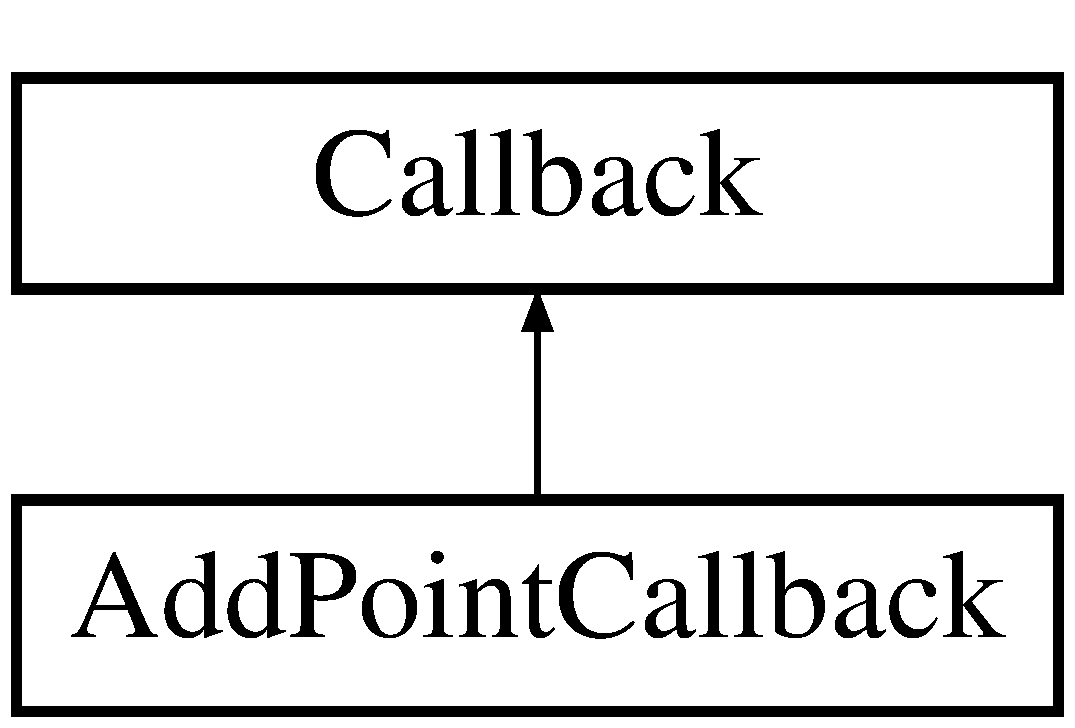
\includegraphics[height=2.000000cm]{structAddPointCallback}
\end{center}
\end{figure}
\subsection*{Public Member Functions}
\begin{DoxyCompactItemize}
\item 
{\bfseries Add\+Point\+Callback} ({\bf S\+B\+L\+Subdivision} \&\+\_\+s)\label{structAddPointCallback_aae0bfd6a9ecd5d7d17b8528998e4f60b}

\item 
virtual void {\bfseries Visit} (Node $\ast$n)\label{structAddPointCallback_a089501f29df7561f5fa80373f104faea}

\end{DoxyCompactItemize}
\subsection*{Public Attributes}
\begin{DoxyCompactItemize}
\item 
{\bf S\+B\+L\+Subdivision} \& {\bfseries s}\label{structAddPointCallback_a229afd715b5ff8ecc308ef267215d879}

\end{DoxyCompactItemize}


The documentation for this struct was generated from the following file\+:\begin{DoxyCompactItemize}
\item 
S\+B\+L\+Tree.\+cpp\end{DoxyCompactItemize}

\section{Bidirectional\+R\+R\+T\+Planner Class Reference}
\label{classBidirectionalRRTPlanner}\index{Bidirectional\+R\+R\+T\+Planner@{Bidirectional\+R\+R\+T\+Planner}}


A single-\/query R\+RT (Rapidly-\/\+Exploring Random Tree) planner.  




{\ttfamily \#include $<$Motion\+Planner.\+h$>$}

Inheritance diagram for Bidirectional\+R\+R\+T\+Planner\+:\begin{figure}[H]
\begin{center}
\leavevmode
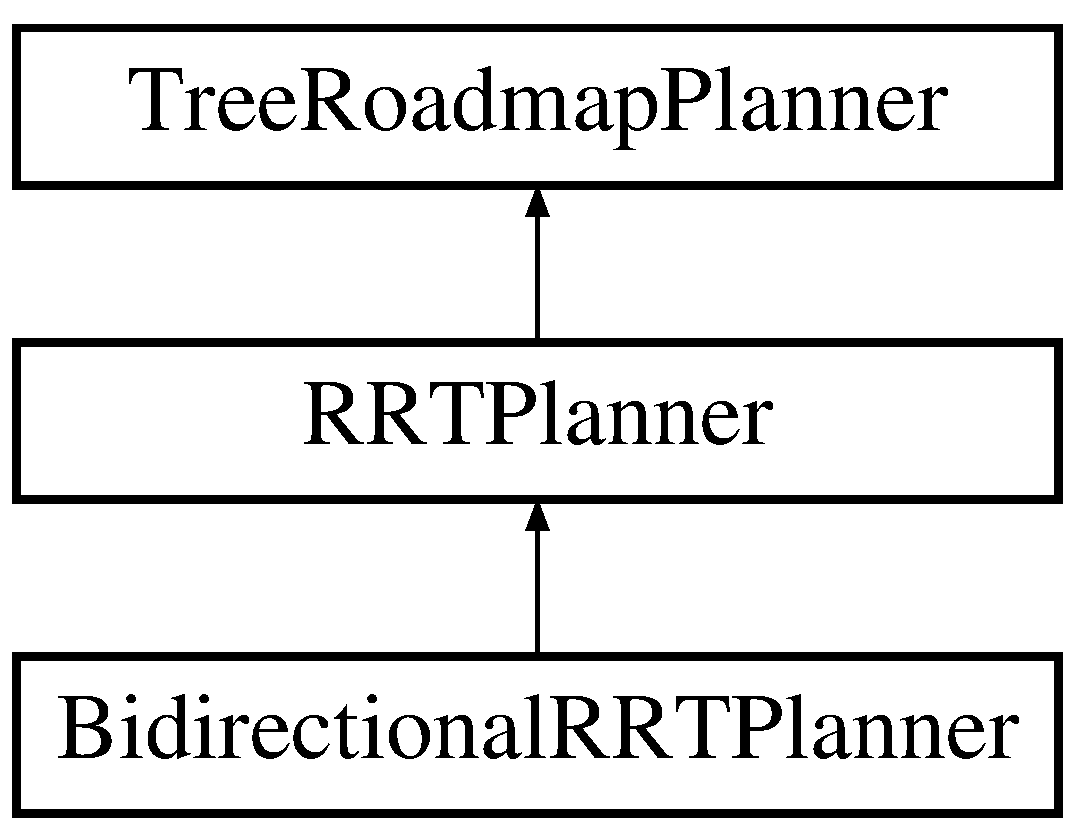
\includegraphics[height=3.000000cm]{classBidirectionalRRTPlanner}
\end{center}
\end{figure}
\subsection*{Public Member Functions}
\begin{DoxyCompactItemize}
\item 
{\bfseries Bidirectional\+R\+R\+T\+Planner} ({\bf C\+Space} $\ast$s)\label{classBidirectionalRRTPlanner_a11d8c99aa3c9e93cae5f03a1f566c654}

\item 
void {\bf Init} (const Config \&start, const Config \&goal)\label{classBidirectionalRRTPlanner_ad87d74d50c4cd273c1ce0ae929412a52}

\begin{DoxyCompactList}\small\item\em Clears the trees, then initializes the start/goal configs. \end{DoxyCompactList}\item 
bool {\bf Plan} ()\label{classBidirectionalRRTPlanner_a78df1be8d25e961f78b39b1e992e07c3}

\begin{DoxyCompactList}\small\item\em Performs 1 step of planning, returns true on success. \end{DoxyCompactList}\item 
void {\bf Create\+Path} ({\bf Milestone\+Path} \&) const \label{classBidirectionalRRTPlanner_a53fbe655860bff1fc9174cedc361c58a}

\begin{DoxyCompactList}\small\item\em Returns the planned path, if successful. \end{DoxyCompactList}\end{DoxyCompactItemize}
\subsection*{Additional Inherited Members}


\subsection{Detailed Description}
A single-\/query R\+RT (Rapidly-\/\+Exploring Random Tree) planner. 

Consists of two trees, one from the start, the other from the goal. Tries to connect the two when an extended config is within connection\+Threshold of the other tree.

The start and goal configs are stored in milestones 0 and 1, resp. 

The documentation for this class was generated from the following files\+:\begin{DoxyCompactItemize}
\item 
Motion\+Planner.\+h\item 
Motion\+Planner.\+cpp\end{DoxyCompactItemize}

\section{Bisection\+Epsilon\+Edge\+Planner Class Reference}
\label{classBisectionEpsilonEdgePlanner}\index{Bisection\+Epsilon\+Edge\+Planner@{Bisection\+Epsilon\+Edge\+Planner}}


{\ttfamily \#include $<$Edge\+Planner.\+h$>$}

Inheritance diagram for Bisection\+Epsilon\+Edge\+Planner\+:\begin{figure}[H]
\begin{center}
\leavevmode
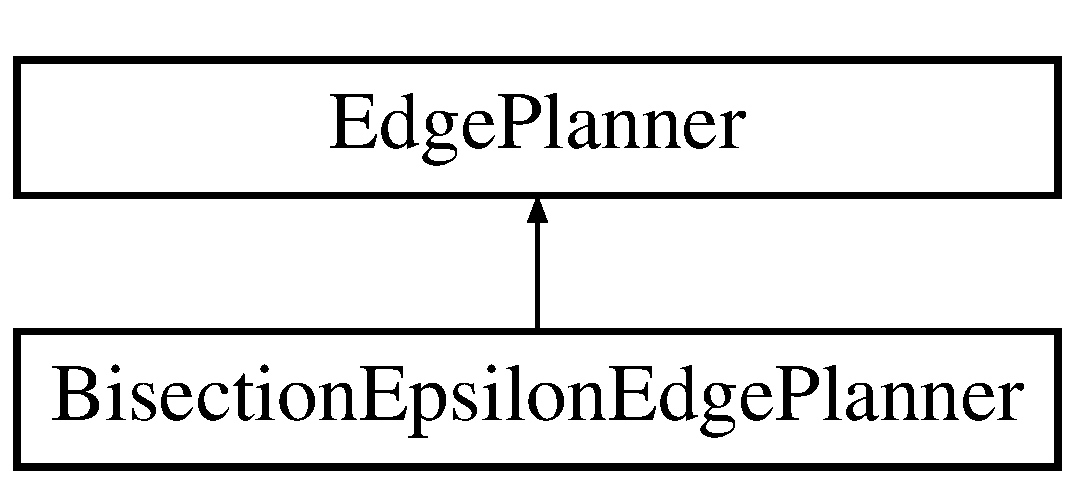
\includegraphics[height=2.000000cm]{classBisectionEpsilonEdgePlanner}
\end{center}
\end{figure}
\subsection*{Classes}
\begin{DoxyCompactItemize}
\item 
struct {\bf Segment}
\end{DoxyCompactItemize}
\subsection*{Public Member Functions}
\begin{DoxyCompactItemize}
\item 
{\bfseries Bisection\+Epsilon\+Edge\+Planner} (const Config \&a, const Config \&b, {\bf C\+Space} $\ast$space, double epsilon)\label{classBisectionEpsilonEdgePlanner_a43111ac77687201b449e3492749f12f1}

\item 
virtual bool {\bfseries Is\+Visible} ()\label{classBisectionEpsilonEdgePlanner_a4a79397d3e7dc828f5886f26ba5f40a2}

\item 
virtual void {\bfseries Eval} (double u, Config \&x) const \label{classBisectionEpsilonEdgePlanner_a72281f1fd4674b17b12116e89ff3c004}

\item 
virtual const Config \& {\bfseries Start} () const \label{classBisectionEpsilonEdgePlanner_ac67a8a18de843c12810545093c6c7b61}

\item 
virtual const Config \& {\bfseries Goal} () const \label{classBisectionEpsilonEdgePlanner_a8cfc460995f4f59d712f87d6bdf0003e}

\item 
virtual {\bf C\+Space} $\ast$ {\bfseries Space} () const \label{classBisectionEpsilonEdgePlanner_aeed5f126ce4befa9b2e068e780df1167}

\item 
virtual {\bf Edge\+Planner} $\ast$ {\bfseries Copy} () const \label{classBisectionEpsilonEdgePlanner_ada406b23e33b944966622432b9eb8bd2}

\item 
virtual {\bf Edge\+Planner} $\ast$ {\bfseries Reverse\+Copy} () const \label{classBisectionEpsilonEdgePlanner_a83b4c90216c06c9701d2b26fe42f5a81}

\item 
virtual double {\bfseries Priority} () const \label{classBisectionEpsilonEdgePlanner_a9122009f2502ed573c43044d316ba8dc}

\item 
virtual bool {\bfseries Plan} ()\label{classBisectionEpsilonEdgePlanner_adeb5fb373547ca70f2563a9366ac4c01}

\item 
virtual bool {\bfseries Done} () const \label{classBisectionEpsilonEdgePlanner_a1acb9bdea6be6f786fe01dffe2959864}

\item 
virtual bool {\bfseries Failed} () const \label{classBisectionEpsilonEdgePlanner_ac6c2917e36c8f26bb6812e156422a501}

\item 
bool {\bfseries Plan} (Config $\ast$\&pre, Config $\ast$\&post)\label{classBisectionEpsilonEdgePlanner_a770bf13d9ca644de26caa054ac5dbf62}

\item 
const std\+::list$<$ Config $>$ \& {\bfseries Get\+Path} () const \label{classBisectionEpsilonEdgePlanner_a5a8690860fbb69edf76ecec85a9017de}

\item 
const Config \& {\bfseries Infeasible\+Config} () const \label{classBisectionEpsilonEdgePlanner_ad8c6b634b64db70c855ae9f35bed9acf}

\end{DoxyCompactItemize}
\subsection*{Protected Member Functions}
\begin{DoxyCompactItemize}
\item 
{\bfseries Bisection\+Epsilon\+Edge\+Planner} ({\bf C\+Space} $\ast$space, double epsilon)\label{classBisectionEpsilonEdgePlanner_abe7adeb27fdabf51095561816be6b5ec}

\end{DoxyCompactItemize}
\subsection*{Protected Attributes}
\begin{DoxyCompactItemize}
\item 
std\+::list$<$ Config $>$ {\bfseries path}\label{classBisectionEpsilonEdgePlanner_aee6809e8a6f1fc5a68404d0cb7b08592}

\item 
{\bf C\+Space} $\ast$ {\bfseries space}\label{classBisectionEpsilonEdgePlanner_a730d7ea663f52421ddbc92976e757ddd}

\item 
double {\bfseries epsilon}\label{classBisectionEpsilonEdgePlanner_a2ab619ed54e73b450ffef7e82defa4b4}

\item 
std\+::priority\+\_\+queue$<$ {\bf Segment}, std\+::vector$<$ {\bf Segment} $>$ $>$ {\bfseries q}\label{classBisectionEpsilonEdgePlanner_a6c81be6c959284703a300fb5c3fdb44c}

\item 
Config {\bfseries x}\label{classBisectionEpsilonEdgePlanner_a54d1bd746c9d0da165c1ba09f1f876df}

\end{DoxyCompactItemize}


\subsection{Detailed Description}
The same as \doxyref{Straight\+Line\+Epsilon\+Planner}{p.}{classStraightLineEpsilonPlanner}, but keeps the bisected configs, and recalculates distances for every subdivision.

Used in constrained configuration spaces where C\+Space.\+Midpoint() doesn\textquotesingle{}t necessarily return a configuration whose distance is half of the endpoints. 

The documentation for this class was generated from the following files\+:\begin{DoxyCompactItemize}
\item 
Edge\+Planner.\+h\item 
Edge\+Planner.\+cpp\end{DoxyCompactItemize}

\section{Bisection\+Epsilon\+Explicit\+Edge\+Planner Class Reference}
\label{classBisectionEpsilonExplicitEdgePlanner}\index{Bisection\+Epsilon\+Explicit\+Edge\+Planner@{Bisection\+Epsilon\+Explicit\+Edge\+Planner}}
Inheritance diagram for Bisection\+Epsilon\+Explicit\+Edge\+Planner\+:\begin{figure}[H]
\begin{center}
\leavevmode
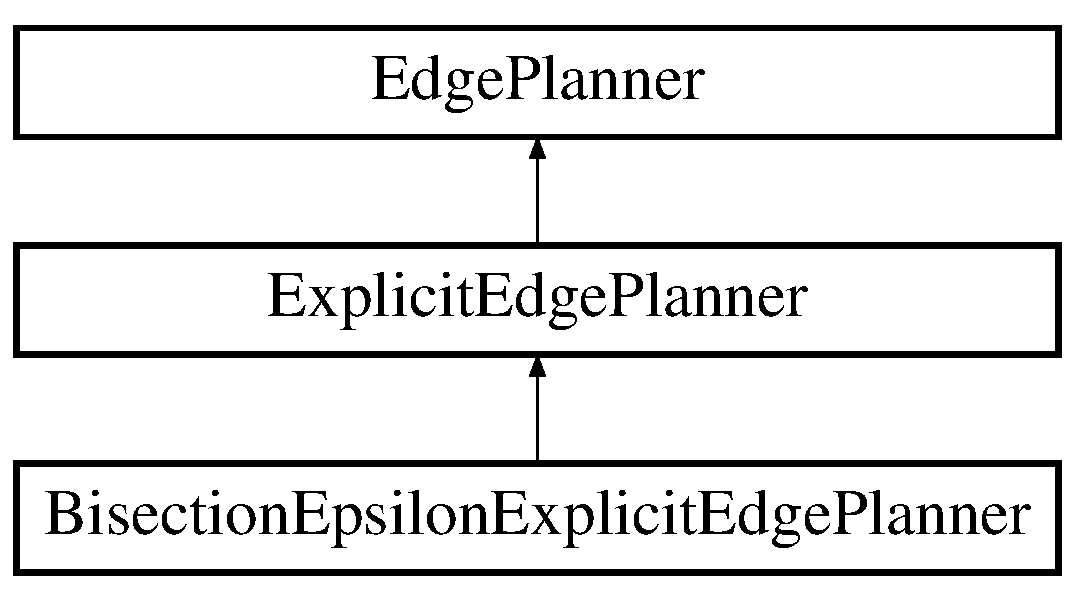
\includegraphics[height=3.000000cm]{classBisectionEpsilonExplicitEdgePlanner}
\end{center}
\end{figure}
\subsection*{Public Member Functions}
\begin{DoxyCompactItemize}
\item 
{\bfseries Bisection\+Epsilon\+Explicit\+Edge\+Planner} ({\bf Explicit\+C\+Space} $\ast$space, const Config \&a, const Config \&b, double eps)\label{classBisectionEpsilonExplicitEdgePlanner_a44bca5a38b91589f3784a3b88892b7ab}

\item 
virtual bool {\bfseries Is\+Visible} ()\label{classBisectionEpsilonExplicitEdgePlanner_ac2075897238afe2a282ba6a3354d0dd2}

\item 
virtual bool {\bfseries Is\+Visible} (int i)\label{classBisectionEpsilonExplicitEdgePlanner_ab69e84eaed85480afd1da44e33475c16}

\item 
virtual void {\bfseries Check\+Visible} (std\+::vector$<$ bool $>$ \&visible)\label{classBisectionEpsilonExplicitEdgePlanner_aefee540b3f2a47605e9b6a01f754a1d6}

\item 
virtual {\bf Edge\+Planner} $\ast$ {\bfseries Copy} () const \label{classBisectionEpsilonExplicitEdgePlanner_ae8e47b97c509edee78d9a2aa61f46476}

\item 
virtual {\bf Edge\+Planner} $\ast$ {\bfseries Reverse\+Copy} () const \label{classBisectionEpsilonExplicitEdgePlanner_a70d1c02b22510d7879543808d99b1aa6}

\item 
bool {\bfseries Plan\+All} ()\label{classBisectionEpsilonExplicitEdgePlanner_aad925f13f59865ff40a1e9598306d23b}

\item 
virtual double {\bfseries Priority} () const \label{classBisectionEpsilonExplicitEdgePlanner_a632d9cfab63a59469ceae16351fc43f6}

\item 
virtual bool {\bfseries Plan} ()\label{classBisectionEpsilonExplicitEdgePlanner_a2ad3e71f42507850a0c265535c8111ad}

\item 
virtual bool {\bfseries Done} () const \label{classBisectionEpsilonExplicitEdgePlanner_a76c4a169bf3262812ec81c0d67754454}

\item 
virtual bool {\bfseries Failed} () const \label{classBisectionEpsilonExplicitEdgePlanner_af3832c15aba3674ba4f247c9536c69d4}

\item 
virtual double {\bfseries Priority} (int i) const \label{classBisectionEpsilonExplicitEdgePlanner_a208461946ce16e7e3460c159712cafd4}

\item 
virtual bool {\bfseries Plan} (int i)\label{classBisectionEpsilonExplicitEdgePlanner_a8c2c51be37bc99800d7efed16522ee69}

\item 
virtual bool {\bfseries Done} (int i) const \label{classBisectionEpsilonExplicitEdgePlanner_a41ecb7929d729bdefc32d34fb33e5ba7}

\item 
virtual bool {\bfseries Failed} (int i) const \label{classBisectionEpsilonExplicitEdgePlanner_a207956fb105a9210e99f04ff47a995e6}

\end{DoxyCompactItemize}
\subsection*{Additional Inherited Members}


The documentation for this class was generated from the following files\+:\begin{DoxyCompactItemize}
\item 
Explicit\+C\+Space.\+h\item 
Explicit\+C\+Space.\+cpp\end{DoxyCompactItemize}

\section{Change\+Tree\+Callback Struct Reference}
\label{structChangeTreeCallback}\index{Change\+Tree\+Callback@{Change\+Tree\+Callback}}
Inheritance diagram for Change\+Tree\+Callback\+:\begin{figure}[H]
\begin{center}
\leavevmode
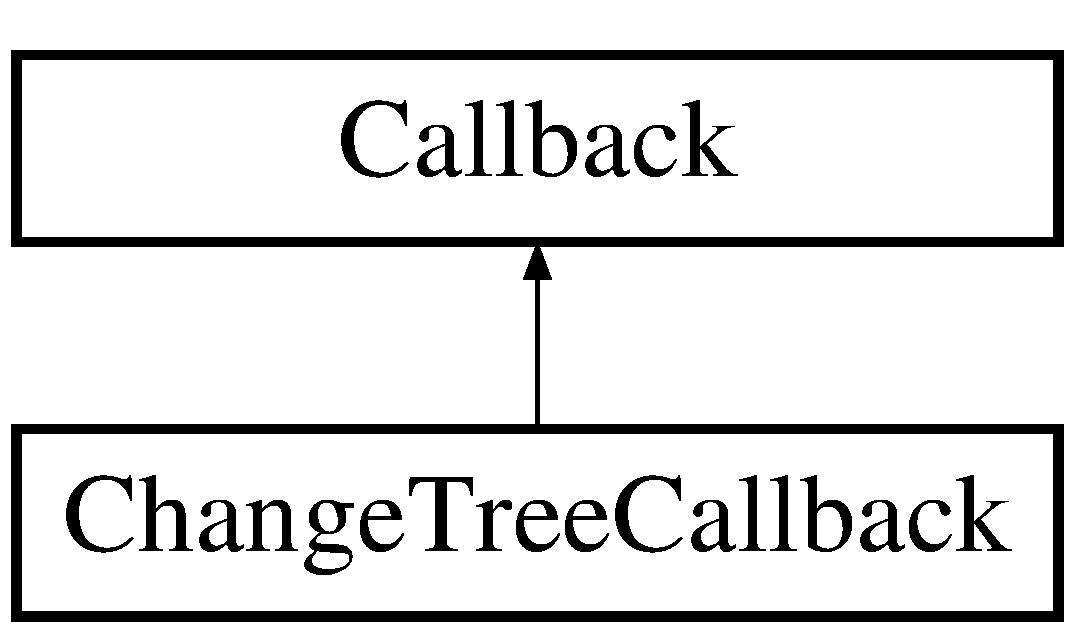
\includegraphics[height=2.000000cm]{structChangeTreeCallback}
\end{center}
\end{figure}
\subsection*{Public Member Functions}
\begin{DoxyCompactItemize}
\item 
{\bfseries Change\+Tree\+Callback} ({\bf S\+B\+L\+Tree} $\ast$\+\_\+a, {\bf S\+B\+L\+Tree} $\ast$\+\_\+b)\label{structChangeTreeCallback_a53d4348299a01338af878e0ccd953d0c}

\item 
virtual void {\bfseries Visit} (Node $\ast$n)\label{structChangeTreeCallback_a3d879482b10c711be3457b69c7338fb4}

\end{DoxyCompactItemize}
\subsection*{Public Attributes}
\begin{DoxyCompactItemize}
\item 
{\bf S\+B\+L\+Tree} $\ast$ {\bfseries a}\label{structChangeTreeCallback_ad9f79b61d010e58f6a781f733770e0e2}

\item 
{\bf S\+B\+L\+Tree} $\ast$ {\bfseries b}\label{structChangeTreeCallback_a95d015b3ab0b0ebd381496992364afc6}

\end{DoxyCompactItemize}


The documentation for this struct was generated from the following file\+:\begin{DoxyCompactItemize}
\item 
S\+B\+L\+Tree.\+cpp\end{DoxyCompactItemize}

\section{Closest\+Milestone\+Callback Struct Reference}
\label{structClosestMilestoneCallback}\index{Closest\+Milestone\+Callback@{Closest\+Milestone\+Callback}}
Inheritance diagram for Closest\+Milestone\+Callback\+:\begin{figure}[H]
\begin{center}
\leavevmode
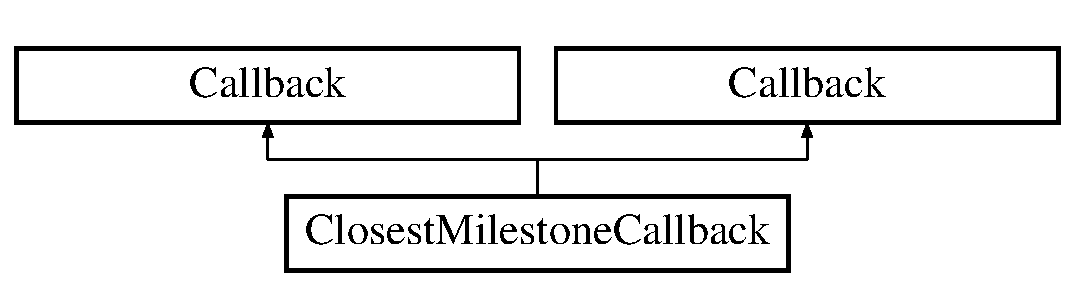
\includegraphics[height=2.000000cm]{structClosestMilestoneCallback}
\end{center}
\end{figure}
\subsection*{Public Member Functions}
\begin{DoxyCompactItemize}
\item 
{\bfseries Closest\+Milestone\+Callback} ({\bf C\+Space} $\ast$s, const Config \&\+\_\+x)\label{structClosestMilestoneCallback_a9f8a444162aa5e03a35e3bb99bf3d4c7}

\item 
virtual void {\bfseries Visit} (Node $\ast$n)\label{structClosestMilestoneCallback_a5bb6282621e11ea803b390ed166a4080}

\item 
{\bfseries Closest\+Milestone\+Callback} ({\bf C\+Space} $\ast$s, const Config \&\+\_\+x)\label{structClosestMilestoneCallback_a9f8a444162aa5e03a35e3bb99bf3d4c7}

\item 
virtual void {\bfseries Visit} (Node $\ast$n)\label{structClosestMilestoneCallback_a5bb6282621e11ea803b390ed166a4080}

\end{DoxyCompactItemize}
\subsection*{Public Attributes}
\begin{DoxyCompactItemize}
\item 
{\bf C\+Space} $\ast$ {\bfseries space}\label{structClosestMilestoneCallback_a0e13d5e2ef219036d553c202c697e6af}

\item 
double {\bfseries closest\+Distance}\label{structClosestMilestoneCallback_af7e5f01ea89c7f6a277c131ed38c3860}

\item 
const Config \& {\bfseries x}\label{structClosestMilestoneCallback_a9884a058f0b28f7934f1b1171c8f123d}

\item 
Node $\ast$ {\bfseries closest\+Milestone}\label{structClosestMilestoneCallback_aef76406c3da34e2ed667fae66bbdba22}

\end{DoxyCompactItemize}


The documentation for this struct was generated from the following files\+:\begin{DoxyCompactItemize}
\item 
Motion\+Planner.\+cpp\item 
S\+B\+L\+Tree.\+cpp\end{DoxyCompactItemize}

\section{Connected\+Seed\+Callback Struct Reference}
\label{structConnectedSeedCallback}\index{Connected\+Seed\+Callback@{Connected\+Seed\+Callback}}
Inheritance diagram for Connected\+Seed\+Callback\+:\begin{figure}[H]
\begin{center}
\leavevmode
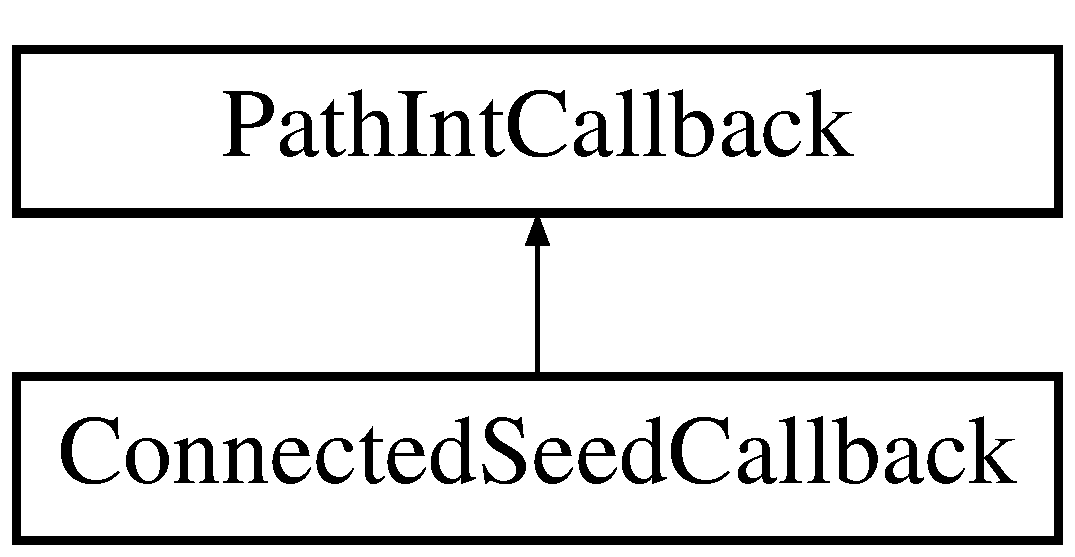
\includegraphics[height=2.000000cm]{structConnectedSeedCallback}
\end{center}
\end{figure}
\subsection*{Public Member Functions}
\begin{DoxyCompactItemize}
\item 
{\bfseries Connected\+Seed\+Callback} ({\bf S\+B\+L\+P\+RT} $\ast$\+\_\+prt, int seeknode)\label{structConnectedSeedCallback_a70c63570cd652c3678ad76c8f6df2052}

\item 
virtual bool {\bfseries Forward\+Edge} (int i, int j)\label{structConnectedSeedCallback_aacfec4449749226a1899e1a068ac71f0}

\end{DoxyCompactItemize}
\subsection*{Public Attributes}
\begin{DoxyCompactItemize}
\item 
{\bf S\+B\+L\+P\+RT} $\ast$ {\bfseries prt}\label{structConnectedSeedCallback_a23e26a269014c9055036068a289fa4e2}

\end{DoxyCompactItemize}


The documentation for this struct was generated from the following file\+:\begin{DoxyCompactItemize}
\item 
S\+B\+L.\+cpp\end{DoxyCompactItemize}

\section{Coverage\+Limited\+Path\+Callback Struct Reference}
\label{structCoverageLimitedPathCallback}\index{Coverage\+Limited\+Path\+Callback@{Coverage\+Limited\+Path\+Callback}}
Inheritance diagram for Coverage\+Limited\+Path\+Callback\+:\begin{figure}[H]
\begin{center}
\leavevmode
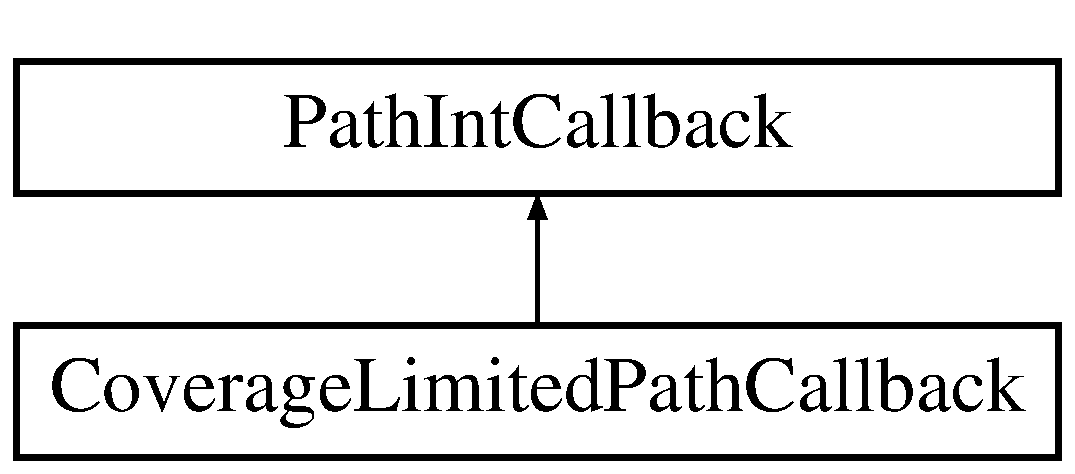
\includegraphics[height=2.000000cm]{structCoverageLimitedPathCallback}
\end{center}
\end{figure}
\subsection*{Public Member Functions}
\begin{DoxyCompactItemize}
\item 
{\bfseries Coverage\+Limited\+Path\+Callback} ({\bf Error\+Explaining\+Planner} $\ast$\+\_\+planner, const {\bf Subset} \&\+\_\+cover, int \+\_\+target=-\/1)\label{structCoverageLimitedPathCallback_aa05c61e1a17a148a5a1d2de16f3d79dc}

\item 
virtual bool {\bfseries Forward\+Edge} (int i, int j)\label{structCoverageLimitedPathCallback_ab60833606c22de4cd5df8fa3bf51b8e9}

\end{DoxyCompactItemize}
\subsection*{Public Attributes}
\begin{DoxyCompactItemize}
\item 
{\bf Error\+Explaining\+Planner} $\ast$ {\bfseries planner}\label{structCoverageLimitedPathCallback_adf8331c5b809401c2059b8e48ea9344a}

\item 
const {\bf Subset} \& {\bfseries cover}\label{structCoverageLimitedPathCallback_a20388649f00268a702767d9442e46e16}

\end{DoxyCompactItemize}


The documentation for this struct was generated from the following file\+:\begin{DoxyCompactItemize}
\item 
Explaining\+Planner.\+cpp\end{DoxyCompactItemize}

\section{C\+Space Class Reference}
\label{classCSpace}\index{C\+Space@{C\+Space}}


Motion planning configuration space base class.  




{\ttfamily \#include $<$C\+Space.\+h$>$}

Inheritance diagram for C\+Space\+:\begin{figure}[H]
\begin{center}
\leavevmode
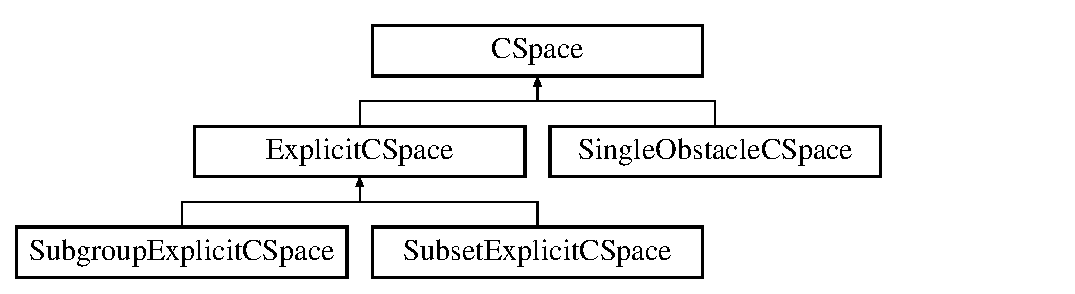
\includegraphics[height=3.000000cm]{classCSpace}
\end{center}
\end{figure}
\subsection*{Public Member Functions}
\begin{DoxyCompactItemize}
\item 
virtual void {\bfseries Sample} (Config \&x)=0\label{classCSpace_a2bac5dcec67c7062d97715f95fd1f858}

\item 
virtual void {\bfseries Sample\+Neighborhood} (const Config \&c, double r, Config \&x)\label{classCSpace_a847aa27ba5a93df085dc1e18faea7981}

\item 
virtual bool {\bfseries Is\+Feasible} (const Config \&)=0\label{classCSpace_a6d207d56ae81349bfb29be035ebc5f4d}

\item 
virtual {\bf Edge\+Planner} $\ast$ {\bfseries Local\+Planner} (const Config \&a, const Config \&b)=0\label{classCSpace_ae36cd1851a14ceebb89f7974f0e0051f}

\item 
virtual double {\bf Distance} (const Config \&x, const Config \&y)\label{classCSpace_a8705829b41ebd6d749a2db6f8404029a}

\begin{DoxyCompactList}\small\item\em optionally overrideable (default uses euclidean space) \end{DoxyCompactList}\item 
virtual void {\bfseries Interpolate} (const Config \&x, const Config \&y, double u, Config \&out)\label{classCSpace_aa87c5b4fd55ba180ebe4072e29b4d1d2}

\item 
virtual double {\bf Obstacle\+Distance} (const Config \&a)\label{classCSpace_a364b5b0ebcc258c39a263914ad3a0a89}

\begin{DoxyCompactList}\small\item\em for local planners using obstacle distance \end{DoxyCompactList}\end{DoxyCompactItemize}


\subsection{Detailed Description}
Motion planning configuration space base class. 

An abstract base class defining the C-\/space interfaces needed for motion planning. The methods represent a configuration as a vector$<$double$>$, but the space may be noneuclidean or not even the same dimensionality as the \# of entries in the configuration.

The Sample, Is\+Feasible, and Local\+Planner methods must be overridden by the subclass. They implicitly define the C-\/space and free space. Sample M\+U\+ST have a nonzero chance of succeeding for any of the motion planning algorithms to work. Local\+Planner will return a new instance of an \doxyref{Edge\+Planner}{p.}{classEdgePlanner} (see \doxyref{Edge\+Planner.\+h}{p.}{EdgePlanner_8h_source}) depending on the desired type of local planner.

The Distance, Interpolate, and Sample\+Neighborhood methods are optionally overrideable; the default implementations assume a Euclidean space. They must be overridden to implement a C-\/space with a noneuclidean topology.

The Obstacle\+Distance method can be overridden to use the \doxyref{Straight\+Line\+Obstacle\+Distance\+Planner}{p.}{classStraightLineObstacleDistancePlanner} local planner (note that this has not been thoroughly tested). 

The documentation for this class was generated from the following files\+:\begin{DoxyCompactItemize}
\item 
C\+Space.\+h\item 
C\+Space.\+cpp\end{DoxyCompactItemize}

\section{Error\+Explaining\+Planner\+:\+:Edge Struct Reference}
\label{structErrorExplainingPlanner_1_1Edge}\index{Error\+Explaining\+Planner\+::\+Edge@{Error\+Explaining\+Planner\+::\+Edge}}
\subsection*{Public Attributes}
\begin{DoxyCompactItemize}
\item 
Smart\+Pointer$<$ {\bf Edge\+Planner} $>$ {\bfseries e}\label{structErrorExplainingPlanner_1_1Edge_a0fd668bcfe7cd6d373b234ac4bbaa5f6}

\item 
int {\bfseries mode}\label{structErrorExplainingPlanner_1_1Edge_ab7d00c2327c0da70fff0b4d6198e6d40}

\end{DoxyCompactItemize}


The documentation for this struct was generated from the following file\+:\begin{DoxyCompactItemize}
\item 
Explaining\+Planner.\+h\end{DoxyCompactItemize}

\section{S\+B\+L\+Tree\+:\+:Edge\+Info Struct Reference}
\label{structSBLTree_1_1EdgeInfo}\index{S\+B\+L\+Tree\+::\+Edge\+Info@{S\+B\+L\+Tree\+::\+Edge\+Info}}
\subsection*{Public Attributes}
\begin{DoxyCompactItemize}
\item 
Node $\ast$ {\bfseries s}\label{structSBLTree_1_1EdgeInfo_ae9ed468cb8fa8294f98b5c356b011884}

\item 
Node $\ast$ {\bfseries t}\label{structSBLTree_1_1EdgeInfo_abaf54b1bb83e819daed62fb5bcf77154}

\item 
Smart\+Pointer$<$ {\bf Edge\+Planner} $>$ {\bfseries e}\label{structSBLTree_1_1EdgeInfo_aee3fe38971af7e2cc9f0ca5fd9262526}

\item 
bool {\bfseries reversed}\label{structSBLTree_1_1EdgeInfo_a42a418024ca5cc58cde77dca8d12a688}

\end{DoxyCompactItemize}


The documentation for this struct was generated from the following file\+:\begin{DoxyCompactItemize}
\item 
S\+B\+L\+Tree.\+h\end{DoxyCompactItemize}

\section{Edge\+Length\+Function Struct Reference}
\label{structEdgeLengthFunction}\index{Edge\+Length\+Function@{Edge\+Length\+Function}}
\subsection*{Public Member Functions}
\begin{DoxyCompactItemize}
\item 
{\bfseries Edge\+Length\+Function} ({\bf Incremental\+M\+M\+P\+R\+M\+\_\+\+Search} $\ast$\+\_\+g)\label{structEdgeLengthFunction_a11ab35ff5ac4b02a358cfb52f245246d}

\item 
double {\bfseries operator()} ({\bf Multi\+Modal\+P\+R\+M\+::\+Transition\+Info} $\ast$e, int s, int t) const \label{structEdgeLengthFunction_ad08896952a7ba77083b886ff40bcb748}

\item 
double {\bfseries operator()} (int s, int t) const \label{structEdgeLengthFunction_a99c55c6fa7407db47749fe462b2738d8}

\end{DoxyCompactItemize}
\subsection*{Public Attributes}
\begin{DoxyCompactItemize}
\item 
{\bf Incremental\+M\+M\+P\+R\+M\+\_\+\+Search} $\ast$ {\bfseries g}\label{structEdgeLengthFunction_a4bcb8c3f8cfedde62109d64dce67d539}

\end{DoxyCompactItemize}


The documentation for this struct was generated from the following file\+:\begin{DoxyCompactItemize}
\item 
Multi\+Modal\+Planner.\+cpp\end{DoxyCompactItemize}

\section{Edge\+Planner Class Reference}
\label{classEdgePlanner}\index{Edge\+Planner@{Edge\+Planner}}


Abstract base class for an edge planner.  




{\ttfamily \#include $<$Edge\+Planner.\+h$>$}

Inheritance diagram for Edge\+Planner\+:\begin{figure}[H]
\begin{center}
\leavevmode
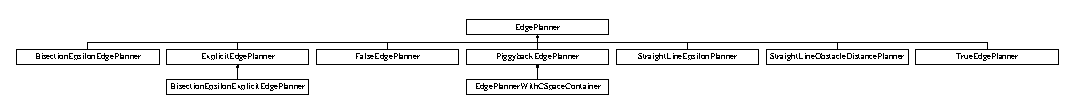
\includegraphics[height=1.043478cm]{classEdgePlanner}
\end{center}
\end{figure}
\subsection*{Public Member Functions}
\begin{DoxyCompactItemize}
\item 
virtual bool {\bfseries Is\+Visible} ()=0\label{classEdgePlanner_a36811a10f49a2b007cae12af1bf39a4d}

\item 
virtual void {\bfseries Eval} (double u, Config \&x) const =0\label{classEdgePlanner_ad866977a4bb25c1453578b7796e99866}

\item 
virtual const Config \& {\bfseries Start} () const =0\label{classEdgePlanner_a8aa4b92bababf31603d57dddfed13737}

\item 
virtual const Config \& {\bfseries Goal} () const =0\label{classEdgePlanner_ae49f00e96cc3fdd2720d4d8df1141130}

\item 
virtual {\bf C\+Space} $\ast$ {\bfseries Space} () const =0\label{classEdgePlanner_a023245383ad18f2a7c61ea6f7ceb8876}

\item 
virtual {\bf Edge\+Planner} $\ast$ {\bfseries Copy} () const =0\label{classEdgePlanner_afe4085b769bffa8cb9a926ffb99d60f4}

\item 
virtual {\bf Edge\+Planner} $\ast$ {\bfseries Reverse\+Copy} () const =0\label{classEdgePlanner_ab105b939eb2920016c5d2e674b77cd58}

\item 
virtual double {\bfseries Priority} () const \label{classEdgePlanner_a77773f4d61e2c7f6a17ef03642707e07}

\item 
virtual bool {\bfseries Plan} ()\label{classEdgePlanner_a5d84b9e80743bf3a3006af65ce75edee}

\item 
virtual bool {\bfseries Done} () const \label{classEdgePlanner_a9e9d54be1a275f31a930457e57e4cbcc}

\item 
virtual bool {\bfseries Failed} () const \label{classEdgePlanner_a0779bdf39860d9819162172279b7bb83}

\end{DoxyCompactItemize}


\subsection{Detailed Description}
Abstract base class for an edge planner. 

N\+O\+TE\+: the only thing allowed to be referenced is the workspace!

Is\+Visible performs the planning process Eval returns the path p(u) with u from 0-\/$>$1. p(0)=a, p(1)=b Start returns p(0) Goal returns p(1) Space() returns the workspace in which this lives Copy returns a copy Reverse\+Copy returns the reverse edge planner

For incremental planners\+: Priority returns some priority measure (such as distance btwn configs) Plan performs one step of the planning process, returns true to continue, false on failure Done returns true if the planning\textquotesingle{}s done 

The documentation for this class was generated from the following file\+:\begin{DoxyCompactItemize}
\item 
Edge\+Planner.\+h\end{DoxyCompactItemize}

\section{Edge\+Planner\+With\+C\+Space\+Container Class Reference}
\label{classEdgePlannerWithCSpaceContainer}\index{Edge\+Planner\+With\+C\+Space\+Container@{Edge\+Planner\+With\+C\+Space\+Container}}


Convenience class for edge planner that holds a smart pointer to a \doxyref{C\+Space}{p.}{classCSpace}. Typically used for single-\/obstacle edge checkers as follows\+:  




{\ttfamily \#include $<$Explicit\+C\+Space.\+h$>$}

Inheritance diagram for Edge\+Planner\+With\+C\+Space\+Container\+:\begin{figure}[H]
\begin{center}
\leavevmode
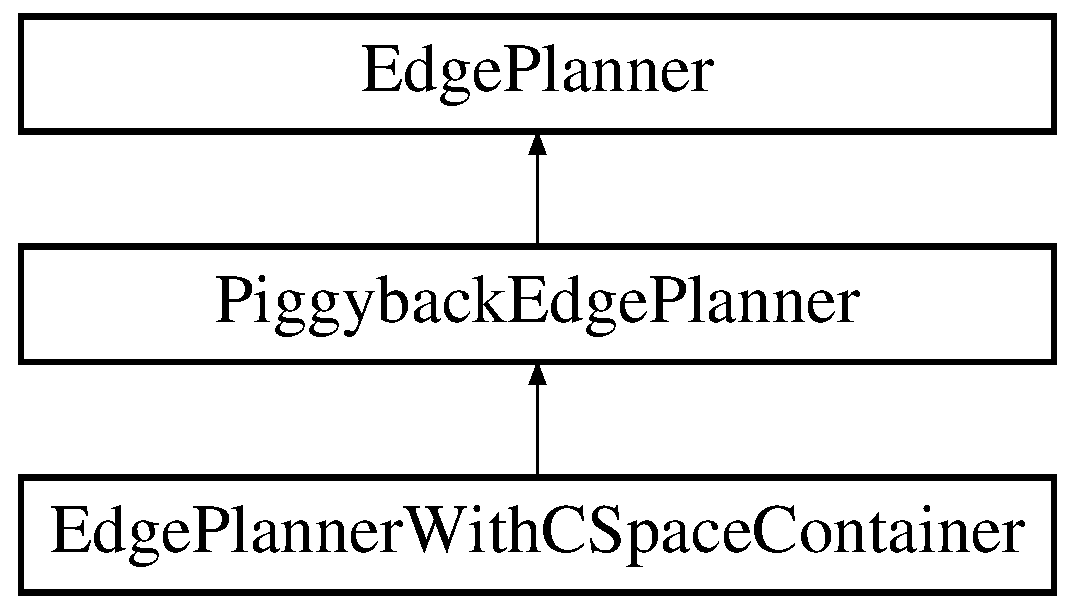
\includegraphics[height=3.000000cm]{classEdgePlannerWithCSpaceContainer}
\end{center}
\end{figure}
\subsection*{Public Member Functions}
\begin{DoxyCompactItemize}
\item 
{\bfseries Edge\+Planner\+With\+C\+Space\+Container} (Smart\+Pointer$<$ {\bf C\+Space} $>$ space, const Smart\+Pointer$<$ {\bf Edge\+Planner} $>$ \&e)\label{classEdgePlannerWithCSpaceContainer_a4768a0a3bc98310e72a2501b70386538}

\item 
virtual {\bf Edge\+Planner} $\ast$ {\bfseries Copy} () const \label{classEdgePlannerWithCSpaceContainer_a2c013c6157b0ef6afda4787c1ffba843}

\item 
virtual {\bf Edge\+Planner} $\ast$ {\bfseries Reverse\+Copy} () const \label{classEdgePlannerWithCSpaceContainer_a5b26a24a02e7c82fd3d2b1eccc6a3001}

\end{DoxyCompactItemize}
\subsection*{Public Attributes}
\begin{DoxyCompactItemize}
\item 
Smart\+Pointer$<$ {\bf C\+Space} $>$ {\bfseries space\+Ptr}\label{classEdgePlannerWithCSpaceContainer_a3297a3f03ef89978e2a60845504620e7}

\end{DoxyCompactItemize}


\subsection{Detailed Description}
Convenience class for edge planner that holds a smart pointer to a \doxyref{C\+Space}{p.}{classCSpace}. Typically used for single-\/obstacle edge checkers as follows\+: 

Single\+Obstacle\+C\+Space$\ast$ ospace = new \doxyref{Single\+Obstacle\+C\+Space(this,obstacle)}{p.}{classSingleObstacleCSpace} return new \doxyref{Edge\+Planner\+With\+C\+Space\+Container(ospace,new X\+Edge\+Planner(ospace,a,b))}{p.}{classEdgePlannerWithCSpaceContainer} 

The documentation for this class was generated from the following files\+:\begin{DoxyCompactItemize}
\item 
Explicit\+C\+Space.\+h\item 
Explicit\+C\+Space.\+cpp\end{DoxyCompactItemize}

\section{Error\+Explaining\+Planner Class Reference}
\label{classErrorExplainingPlanner}\index{Error\+Explaining\+Planner@{Error\+Explaining\+Planner}}


A planner that minimizes the the number of violated constraints using a R\+R\+T-\/like strategy.  




{\ttfamily \#include $<$Explaining\+Planner.\+h$>$}

\subsection*{Classes}
\begin{DoxyCompactItemize}
\item 
struct {\bf Edge}
\item 
struct {\bf Milestone}
\item 
struct {\bf Mode}
\item 
struct {\bf Transition}
\end{DoxyCompactItemize}
\subsection*{Public Types}
\begin{DoxyCompactItemize}
\item 
typedef Graph\+::\+Undirected\+Graph$<$ {\bf Milestone}, {\bf Edge} $>$ {\bfseries Roadmap}\label{classErrorExplainingPlanner_a56a91197e0aeeacb930c863d24d8417c}

\item 
typedef Graph\+::\+Undirected\+Graph$<$ {\bf Mode}, {\bf Transition} $>$ {\bfseries Mode\+Graph}\label{classErrorExplainingPlanner_a19438e7fd028014fb5987103bac79dc7}

\end{DoxyCompactItemize}
\subsection*{Public Member Functions}
\begin{DoxyCompactItemize}
\item 
{\bfseries Error\+Explaining\+Planner} ({\bf Explicit\+C\+Space} $\ast$space)\label{classErrorExplainingPlanner_a963e2f23107efb7f09bac091cc94fcd6}

\item 
void {\bfseries Init} (const Config \&start, const Config \&goal)\label{classErrorExplainingPlanner_a9b143608845d8b292fbb52adb34ed559}

\item 
void {\bf Expand} (double max\+Explanation\+Cost, vector$<$ int $>$ \&new\+Nodes)\label{classErrorExplainingPlanner_af90a5f10d6c872f90f3e0c3506275e5f}

\begin{DoxyCompactList}\small\item\em Performs one iteration of planning given a limit on the explanation size. \end{DoxyCompactList}\item 
void {\bfseries Expand2} (double max\+Explanation\+Cost, vector$<$ int $>$ \&new\+Nodes)\label{classErrorExplainingPlanner_ab5a73133273b1bd5be3de9f458e7e4f6}

\item 
void {\bf Plan} (int initial\+Limit, const vector$<$ int $>$ \&expansion\+Schedule, vector$<$ int $>$ \&best\+Path, {\bf Subset} \&cover)\label{classErrorExplainingPlanner_ac54a2340ac78338394e94b19e2204868}

\begin{DoxyCompactList}\small\item\em Performs bottom-\/up planning according to a given limit expansion schedule. \end{DoxyCompactList}\item 
void {\bf Build\+Roadmap} (double max\+Explanation\+Cost, {\bf Roadmap\+Planner} \&prm)\label{classErrorExplainingPlanner_aa9271ec1fd80dfdce0890e6422bef5d6}

\begin{DoxyCompactList}\small\item\em Outputs the graph with the given explanation limit. \end{DoxyCompactList}\item 
void {\bf Build\+C\+C\+Graph} (Graph\+::\+Undirected\+Graph$<$ {\bf Subset}, int $>$ \&G)
\item 
bool {\bf Coverage\+Path} (int s, int t, const {\bf Subset} \&cover, std\+::vector$<$ int $>$ \&path, {\bf Subset} \&path\+Cover)\label{classErrorExplainingPlanner_a86a3cbc2b423a0ddf4149a443fa4260c}

\begin{DoxyCompactList}\small\item\em A search that finds a path subject to a coverage constraint. \end{DoxyCompactList}\item 
bool {\bf Greedy\+Path} (int s, int t, std\+::vector$<$ int $>$ \&path, {\bf Subset} \&path\+Cover)\label{classErrorExplainingPlanner_af66cfd5b8c6694077e7342c83e2e6391}

\begin{DoxyCompactList}\small\item\em A greedy heuristic that performs smallest cover given predecessor. \end{DoxyCompactList}\item 
bool {\bf Optimal\+Path} (int s, int t, std\+::vector$<$ int $>$ \&path, {\bf Subset} \&path\+Cover)\label{classErrorExplainingPlanner_a7de2fe0b0046e2cd48d3dc87aed72980}

\begin{DoxyCompactList}\small\item\em An optimal search. \end{DoxyCompactList}\item 
void {\bf Completion} (int s, int node, int t, {\bf Subset} \&path\+Cover)
\item 
int {\bfseries Add\+Node} (const Config \&q, int parent=-\/1)\label{classErrorExplainingPlanner_aa72cf7cb49296db4e7a7107c861e0d26}

\item 
int {\bfseries Add\+Node} (const Config \&q, const {\bf Subset} \&subset, int parent=-\/1)\label{classErrorExplainingPlanner_a56b0332f92d518ada526b4053e4f1208}

\item 
bool {\bfseries Add\+Edge} (int i, int j, int depth=0)\label{classErrorExplainingPlanner_a84089ded0070b0af47102054673896b7}

\item 
int {\bfseries Add\+Edge} (int i, const Config \&q, double max\+Explanation\+Cost)\label{classErrorExplainingPlanner_abc71458821dbee70b01b439ad4fe7b65}

\item 
void {\bfseries Add\+Edge\+Raw} (int i, int j)\label{classErrorExplainingPlanner_abf85b58236537b30264bedb67a7bcc5e}

\item 
int {\bfseries Extend\+Toward} (int i, const Config \&qdest, double max\+Explanation\+Cost)\label{classErrorExplainingPlanner_af464c89593cd365067fb153cd7933c2d}

\item 
void {\bfseries K\+NN} (const Config \&q, int k, vector$<$ int $>$ \&neighbors, vector$<$ double $>$ \&distances)\label{classErrorExplainingPlanner_a9a6d147d6c7db3e1c35595e61c9c0292}

\item 
void {\bfseries K\+NN} (const Config \&q, double max\+Explanation\+Cost, int k, vector$<$ int $>$ \&neighbors, vector$<$ double $>$ \&distances)\label{classErrorExplainingPlanner_a01f0d948471c9dafede5242ff38b55af}

\item 
void {\bfseries Update\+Paths\+Greedy} ()\label{classErrorExplainingPlanner_aec5d15d7817421b6828f7c80a296cfac}

\item 
void {\bfseries Update\+Paths\+Complete} ()\label{classErrorExplainingPlanner_ad6162b4799cb486683768ad91a8bc4e1}

\item 
void {\bfseries Update\+Paths\+Greedy2} (int nstart=-\/1)\label{classErrorExplainingPlanner_a0177c9d7ecbd1208a57c4c2dd359f90e}

\item 
void {\bfseries Update\+Paths\+Complete2} (int nstart=-\/1)\label{classErrorExplainingPlanner_af022570650fb2c25b481b6cc6d837d77}

\item 
bool {\bfseries Can\+Improve\+Connectivity} (const {\bf Mode} \&ma, const {\bf Mode} \&mb, double max\+Explanation\+Cost)\label{classErrorExplainingPlanner_a1f139b5e9ce26df3aaea9854ef9b5729}

\item 
void {\bfseries Update\+Min\+Cost} ({\bf Mode} \&m)\label{classErrorExplainingPlanner_a0a75036676a2d69da2c4c868c0ae0ae3}

\item 
bool {\bfseries Exceeds\+Cost\+Limit} (const Config \&q, double limit, {\bf Subset} \&violations)\label{classErrorExplainingPlanner_a0b4cfea304bd3d342a20a22633d715f2}

\item 
bool {\bfseries Exceeds\+Cost\+Limit} (const Config \&a, const Config \&b, double limit, {\bf Subset} \&violations)\label{classErrorExplainingPlanner_a0666ee1b80dbe225c444effddab9b27c}

\item 
void {\bf Get\+Cover} (const std\+::vector$<$ int $>$ \&path, {\bf Subset} \&cover) const \label{classErrorExplainingPlanner_a57481d8a20c85f7a0038f4edd476ce99}

\begin{DoxyCompactList}\small\item\em Computes the cover of the path. \end{DoxyCompactList}\item 
double {\bf Get\+Length} (const std\+::vector$<$ int $>$ \&path) const \label{classErrorExplainingPlanner_aff9ce6e86add017d92f682279a3aedd9}

\begin{DoxyCompactList}\small\item\em Computes the length of the path. \end{DoxyCompactList}\item 
void {\bf Get\+Milestone\+Path} (const std\+::vector$<$ int $>$ \&path, {\bf Milestone\+Path} \&mpath) const \label{classErrorExplainingPlanner_a40339c8dc31a885219cedbe7ad7436ea}

\begin{DoxyCompactList}\small\item\em Returns the \doxyref{Milestone\+Path}{p.}{classMilestonePath}. \end{DoxyCompactList}\end{DoxyCompactItemize}
\subsection*{Public Attributes}
\begin{DoxyCompactItemize}
\item 
Config {\bfseries start}\label{classErrorExplainingPlanner_a36710bec79a3c173e00251824b95e308}

\item 
Config {\bfseries goal}\label{classErrorExplainingPlanner_a0f1ee95b083257d4796d521d774fa51d}

\item 
{\bf Explicit\+C\+Space} $\ast$ {\bfseries space}\label{classErrorExplainingPlanner_a75c47d130fc3bc512d8b283d0912613a}

\item 
vector$<$ double $>$ {\bfseries obstacle\+Weights}\label{classErrorExplainingPlanner_a0250afa4a9a2c93141b2fd1c6b28fb01}

\item 
int {\bfseries num\+Connections}\label{classErrorExplainingPlanner_a6e555e21c3c00c384424048c8f8c52ac}

\item 
double {\bfseries connect\+Threshold}\label{classErrorExplainingPlanner_a21d7c5839299d301a174724b64024c14}

\item 
double {\bfseries expand\+Distance}\label{classErrorExplainingPlanner_a17c0f6473443542ffadf27086be7185a}

\item 
double {\bfseries goal\+Connect\+Threshold}\label{classErrorExplainingPlanner_a9f6484c6c8869f583adf274b8fdaf776}

\item 
double {\bfseries goal\+Bias\+Probability}\label{classErrorExplainingPlanner_a72c15b68e2c34a603d45ecf9bfaf07cb}

\item 
bool {\bfseries bidirectional}\label{classErrorExplainingPlanner_a0e7f0e4e2c7011a2d0aa5a0bcaf2b2c5}

\item 
bool {\bf update\+Paths\+Complete}
\item 
bool {\bf update\+Paths\+Dynamic}
\item 
int {\bf update\+Paths\+Max}\label{classErrorExplainingPlanner_a0345a79ae72d35d183aa8e7205d9f172}

\begin{DoxyCompactList}\small\item\em For complete planning, keep at most this number of covers. \end{DoxyCompactList}\item 
Roadmap {\bfseries roadmap}\label{classErrorExplainingPlanner_a612495ad8eb97c5c2f605364951bf6c3}

\item 
Mode\+Graph {\bfseries mode\+Graph}\label{classErrorExplainingPlanner_ae74e086d9592dbfe5d0ffed9c82ab523}

\item 
int {\bfseries num\+Expands}\label{classErrorExplainingPlanner_a8699e7193a8ed126daf4db6ee4f1db60}

\item 
int {\bfseries num\+Refinement\+Attempts}\label{classErrorExplainingPlanner_ac5fa50b3c9cd6bb0dbe8955d5878f71d}

\item 
int {\bfseries num\+Refinement\+Successes}\label{classErrorExplainingPlanner_ad013d6c851e96bbdd54c66e344705d34}

\item 
int {\bfseries num\+Exploration\+Attempts}\label{classErrorExplainingPlanner_a136fc358adae45ee520c909473e2577e}

\item 
int {\bfseries num\+Edge\+Checks}\label{classErrorExplainingPlanner_a583ba35f3678a68f441cb65f098f2e52}

\item 
int {\bfseries num\+Config\+Checks}\label{classErrorExplainingPlanner_aac3671d266092f7ae843c0ece1044155}

\item 
int {\bfseries num\+Update\+Paths}\label{classErrorExplainingPlanner_a3a09aed18aed703e30c74730d2433d56}

\item 
int {\bfseries num\+Update\+Paths\+Iterations}\label{classErrorExplainingPlanner_a32008e0f8ecbec0fa4227084b51a1ec2}

\item 
double {\bfseries time\+Nearest\+Neighbors}\label{classErrorExplainingPlanner_a26946eda4d7386ece2e9b9007d3618fc}

\item 
double {\bfseries time\+Refine}\label{classErrorExplainingPlanner_abffa295cf9c8f021899b90d1492fcdb5}

\item 
double {\bfseries time\+Explore}\label{classErrorExplainingPlanner_a094f5c7bb8a4712dd75fa2b31333c11a}

\item 
double {\bfseries time\+Update\+Paths}\label{classErrorExplainingPlanner_ae2670819406a22ea3676ba10e6e02fb9}

\item 
double {\bfseries time\+Overhead}\label{classErrorExplainingPlanner_aba2c294091721d4524f3c918028b2400}

\end{DoxyCompactItemize}


\subsection{Detailed Description}
A planner that minimizes the the number of violated constraints using a R\+R\+T-\/like strategy. 

Usage\+: //first, set up \doxyref{Explicit\+C\+Space}{p.}{classExplicitCSpace} cspace. \doxyref{Error\+Explaining\+Planner}{p.}{classErrorExplainingPlanner} planner(\&cspace); planner.\+Init(start,goal);

//do planning with a given expansion schedule vector$<$int$>$ schedule; schedule.\+push\+\_\+back(limit1); ... schedule.\+push\+\_\+back(limit\+N); \doxyref{Subset}{p.}{structSubset} cover; vector$<$int$>$ best\+Plan; planner.\+Plan(0,schedule,best\+Plan,cover);

//output best path \doxyref{Milestone\+Path}{p.}{classMilestonePath} path; planner.\+Get\+Milestone\+Path(best\+Plan,path); 

\subsection{Member Function Documentation}
\index{Error\+Explaining\+Planner@{Error\+Explaining\+Planner}!Build\+C\+C\+Graph@{Build\+C\+C\+Graph}}
\index{Build\+C\+C\+Graph@{Build\+C\+C\+Graph}!Error\+Explaining\+Planner@{Error\+Explaining\+Planner}}
\subsubsection[{Build\+C\+C\+Graph(\+Graph\+::\+Undirected\+Graph$<$ Subset, int $>$ \&\+G)}]{\setlength{\rightskip}{0pt plus 5cm}void Error\+Explaining\+Planner\+::\+Build\+C\+C\+Graph (
\begin{DoxyParamCaption}
\item[{Graph\+::\+Undirected\+Graph$<$ {\bf Subset}, int $>$ \&}]{G}
\end{DoxyParamCaption}
)}\label{classErrorExplainingPlanner_aca8246e074c382a5536cdbf74fa327cb}
Outputs the CC graph. Each node is a connected component of the roadmap within the same subset. \index{Error\+Explaining\+Planner@{Error\+Explaining\+Planner}!Completion@{Completion}}
\index{Completion@{Completion}!Error\+Explaining\+Planner@{Error\+Explaining\+Planner}}
\subsubsection[{Completion(int s, int node, int t, Subset \&path\+Cover)}]{\setlength{\rightskip}{0pt plus 5cm}void Error\+Explaining\+Planner\+::\+Completion (
\begin{DoxyParamCaption}
\item[{int}]{s, }
\item[{int}]{node, }
\item[{int}]{t, }
\item[{{\bf Subset} \&}]{path\+Cover}
\end{DoxyParamCaption}
)}\label{classErrorExplainingPlanner_a17cb8b7a0a5306e39b2cd8de8cb4f46d}
Returns the cover of the path from s-\/$>$node + completion(node,goal) where the path cover is determined using the greedy heuristic 

\subsection{Member Data Documentation}
\index{Error\+Explaining\+Planner@{Error\+Explaining\+Planner}!update\+Paths\+Complete@{update\+Paths\+Complete}}
\index{update\+Paths\+Complete@{update\+Paths\+Complete}!Error\+Explaining\+Planner@{Error\+Explaining\+Planner}}
\subsubsection[{update\+Paths\+Complete}]{\setlength{\rightskip}{0pt plus 5cm}bool Error\+Explaining\+Planner\+::update\+Paths\+Complete}\label{classErrorExplainingPlanner_a6d2910d5ce604fcedf63cccfe3d738bb}
If true\+: use the slower complete, exact cover update. If false\+: use the faster greedy one. \index{Error\+Explaining\+Planner@{Error\+Explaining\+Planner}!update\+Paths\+Dynamic@{update\+Paths\+Dynamic}}
\index{update\+Paths\+Dynamic@{update\+Paths\+Dynamic}!Error\+Explaining\+Planner@{Error\+Explaining\+Planner}}
\subsubsection[{update\+Paths\+Dynamic}]{\setlength{\rightskip}{0pt plus 5cm}bool Error\+Explaining\+Planner\+::update\+Paths\+Dynamic}\label{classErrorExplainingPlanner_a1b15bc2f0799c23537650c53e1ad0b99}
If true\+: do dynamic shortest paths update If false\+: do batch updates when needed 

The documentation for this class was generated from the following files\+:\begin{DoxyCompactItemize}
\item 
Explaining\+Planner.\+h\item 
Explaining\+Planner.\+cpp\end{DoxyCompactItemize}

\section{Explicit\+C\+Space Class Reference}
\label{classExplicitCSpace}\index{Explicit\+C\+Space@{Explicit\+C\+Space}}


Configuration space that exposes N obstacle checks. This functionality can be used in a motion planner to speed up planning by delaying certain expensive obstacle checks, or to provide reasons for infeasibility.  




{\ttfamily \#include $<$Explicit\+C\+Space.\+h$>$}

Inheritance diagram for Explicit\+C\+Space\+:\begin{figure}[H]
\begin{center}
\leavevmode
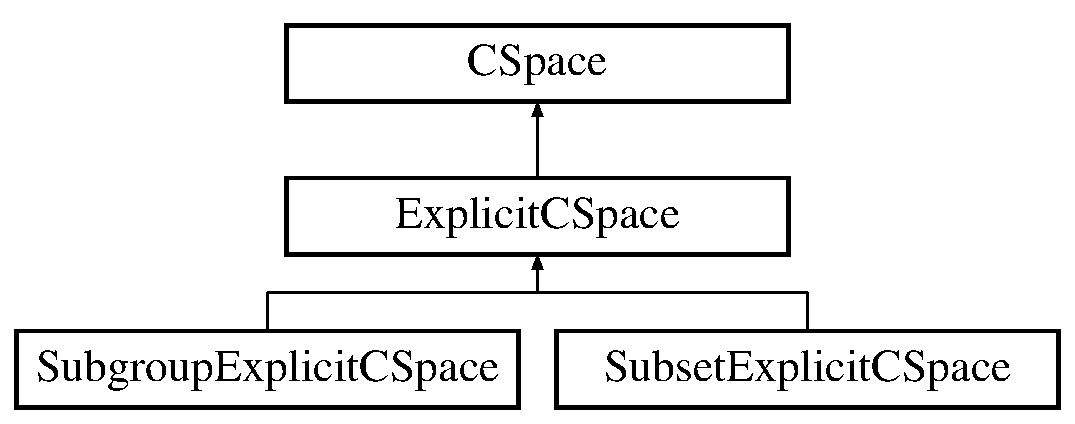
\includegraphics[height=3.000000cm]{classExplicitCSpace}
\end{center}
\end{figure}
\subsection*{Public Member Functions}
\begin{DoxyCompactItemize}
\item 
virtual bool {\bf Is\+Feasible} (const Config \&, int obstacle)=0\label{classExplicitCSpace_ae1a5a6527f51540d0915c55070e63b43}

\begin{DoxyCompactList}\small\item\em Implement this\+: single-\/obstacle feasibility check. \end{DoxyCompactList}\item 
virtual {\bf Edge\+Planner} $\ast$ {\bf Local\+Planner} (const Config \&a, const Config \&b)\label{classExplicitCSpace_a4fea2d3da0e4125319ab4a5db16f2f77}

\begin{DoxyCompactList}\small\item\em Implement this (optional)\+: all obstacle local planner. \end{DoxyCompactList}\item 
virtual {\bf Edge\+Planner} $\ast$ {\bf Local\+Planner} (const Config \&a, const Config \&b, int obstacle)=0\label{classExplicitCSpace_a2ae0ef15db0721388b3919807e79b5ee}

\begin{DoxyCompactList}\small\item\em Implement this\+: single-\/obstacle local planner. \end{DoxyCompactList}\item 
virtual int {\bf Num\+Obstacles} ()=0\label{classExplicitCSpace_a900a2f27b3916706e45df799dc99c16e}

\begin{DoxyCompactList}\small\item\em Implement this\+: returns the number of obstacles. \end{DoxyCompactList}\item 
virtual std\+::string {\bf Obstacle\+Name} (int obstacle)\label{classExplicitCSpace_a9674c8231f71787a758f43761c0f86ec}

\begin{DoxyCompactList}\small\item\em Implement this\+: returns the name of obstacle. \end{DoxyCompactList}\item 
virtual double {\bf Obstacle\+Distance} (const Config \&a, int obstacle)\label{classExplicitCSpace_a27934dc5bd43781295e2302e56e8e71b}

\begin{DoxyCompactList}\small\item\em Optional\+: for local planners using obstacle distance. \end{DoxyCompactList}\item 
virtual bool {\bf Is\+Feasible} (const Config \&)
\item 
virtual void {\bf Check\+Obstacles} (const Config \&, std\+::vector$<$ bool $>$ \&infeasible)\label{classExplicitCSpace_acee7a0d28f2f4f2b696a197d594f0101}

\begin{DoxyCompactList}\small\item\em Returns a vector indicating which obstacles are violated. \end{DoxyCompactList}\end{DoxyCompactItemize}


\subsection{Detailed Description}
Configuration space that exposes N obstacle checks. This functionality can be used in a motion planner to speed up planning by delaying certain expensive obstacle checks, or to provide reasons for infeasibility. 

Subclasses must implement \doxyref{Num\+Obstacles()}{p.}{classExplicitCSpace_a900a2f27b3916706e45df799dc99c16e}, Is\+Feasible(q,i), and Local\+Planner(a,b,i) at a minimum. Many planners will also expect subclasses to implement Local\+Planner(a,b) to return a subclass of \doxyref{Explicit\+Edge\+Planner}{p.}{classExplicitEdgePlanner}. The default implementation of \doxyref{Explicit\+Edge\+Planner}{p.}{classExplicitEdgePlanner} should suffice as long as the obstacle-\/specific Local\+Planner(a,b,i) is implemented. In other words, \char`\"{}return new Explicit\+Edge\+Planner(this,a,b);\char`\"{} 

\subsection{Member Function Documentation}
\index{Explicit\+C\+Space@{Explicit\+C\+Space}!Is\+Feasible@{Is\+Feasible}}
\index{Is\+Feasible@{Is\+Feasible}!Explicit\+C\+Space@{Explicit\+C\+Space}}
\subsubsection[{Is\+Feasible(const Config \&)}]{\setlength{\rightskip}{0pt plus 5cm}bool Explicit\+C\+Space\+::\+Is\+Feasible (
\begin{DoxyParamCaption}
\item[{const Config \&}]{q}
\end{DoxyParamCaption}
)\hspace{0.3cm}{\ttfamily [virtual]}}\label{classExplicitCSpace_a82537edf516ece36a5326a949ba90a37}
Default implementation runs Is\+Feasible(q,index) in order until one is found false 

Implements {\bf C\+Space} \doxyref{}{p.}{classCSpace}.



The documentation for this class was generated from the following files\+:\begin{DoxyCompactItemize}
\item 
Explicit\+C\+Space.\+h\item 
Explicit\+C\+Space.\+cpp\end{DoxyCompactItemize}

\section{Explicit\+Edge\+Planner Class Reference}
\label{classExplicitEdgePlanner}\index{Explicit\+Edge\+Planner@{Explicit\+Edge\+Planner}}


Default edge planner\+: checks each constraint sequentially using the space\textquotesingle{}s Local\+Planner(a,b,i) method.  




{\ttfamily \#include $<$Explicit\+C\+Space.\+h$>$}

Inheritance diagram for Explicit\+Edge\+Planner\+:\begin{figure}[H]
\begin{center}
\leavevmode
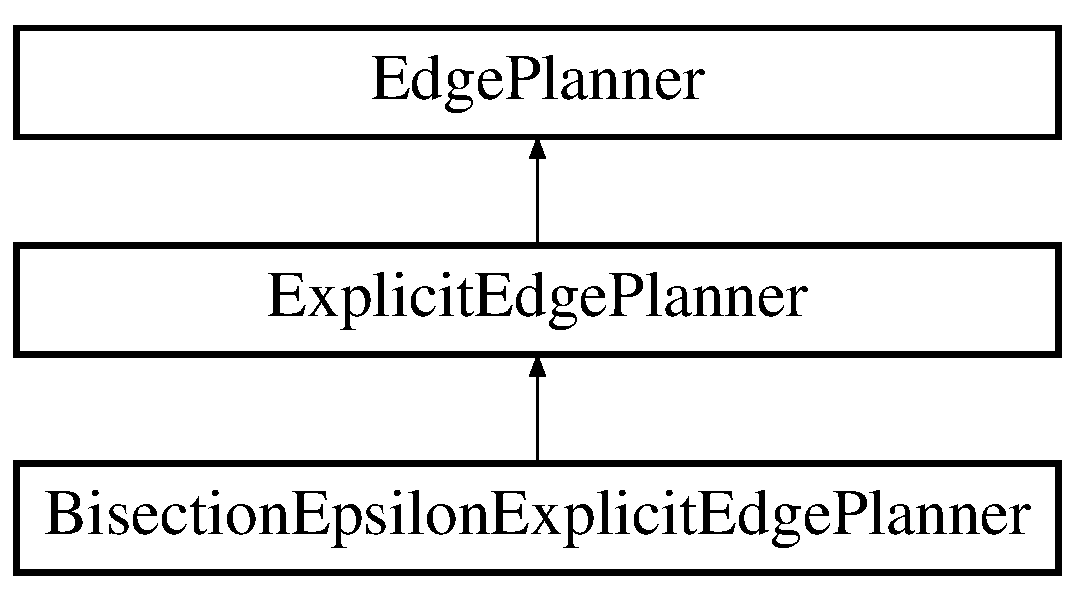
\includegraphics[height=3.000000cm]{classExplicitEdgePlanner}
\end{center}
\end{figure}
\subsection*{Public Member Functions}
\begin{DoxyCompactItemize}
\item 
{\bfseries Explicit\+Edge\+Planner} ({\bf Explicit\+C\+Space} $\ast$space, const Config \&a, const Config \&b, bool init=true)\label{classExplicitEdgePlanner_a7fc6a9c3fbc0e4f207da6064c9c4df72}

\item 
virtual bool {\bfseries Is\+Visible} ()\label{classExplicitEdgePlanner_a7873eb9ad5597113338c5734a3dd03c2}

\item 
virtual bool {\bfseries Is\+Visible} (int i)\label{classExplicitEdgePlanner_a9fc5016e083f7865a52c3fa63b42a191}

\item 
virtual void {\bfseries Check\+Visible} (std\+::vector$<$ bool $>$ \&visible)\label{classExplicitEdgePlanner_a2c90b7e4529a189c13d89df0539e700a}

\item 
virtual void {\bfseries Eval} (double u, Config \&x) const \label{classExplicitEdgePlanner_a91a17a13a7a3d2495ac3b00412d04cdb}

\item 
virtual const Config \& {\bfseries Start} () const \label{classExplicitEdgePlanner_ade0d4aaf20fde1c03e3737b71d2ac032}

\item 
virtual const Config \& {\bfseries Goal} () const \label{classExplicitEdgePlanner_a4a60813bd0d83e9ca0b387aac5834a62}

\item 
virtual {\bf C\+Space} $\ast$ {\bfseries Space} () const \label{classExplicitEdgePlanner_a3fa395c82f553d4fdfc730ad271aa90e}

\item 
virtual {\bf Edge\+Planner} $\ast$ {\bfseries Copy} () const \label{classExplicitEdgePlanner_af761565d7a676e321e06f4464b67a7a4}

\item 
virtual {\bf Edge\+Planner} $\ast$ {\bfseries Reverse\+Copy} () const \label{classExplicitEdgePlanner_a4073c6d786fa30e4997e6e3819b197f2}

\item 
bool {\bfseries Plan\+All} ()\label{classExplicitEdgePlanner_aff439370c5ce1270049b623a4817dfaf}

\item 
virtual double {\bfseries Priority} () const \label{classExplicitEdgePlanner_a03b16719f5f7cbc4bfe539bcf13ea68b}

\item 
virtual bool {\bfseries Plan} ()\label{classExplicitEdgePlanner_a7fe703e011dc50baee57d0f95c35b7d1}

\item 
virtual bool {\bfseries Done} () const \label{classExplicitEdgePlanner_ace8478b1ded61da2c1d0c3ed794c947d}

\item 
virtual bool {\bfseries Failed} () const \label{classExplicitEdgePlanner_ab834b2daedd5cdadc8421afd16728687}

\item 
virtual double {\bfseries Priority} (int i) const \label{classExplicitEdgePlanner_aeb6d901af7c78818322a46e2fc5d0560}

\item 
virtual bool {\bfseries Plan} (int i)\label{classExplicitEdgePlanner_ac22ea5a960d67825c600cd39ee1fedde}

\item 
virtual bool {\bfseries Done} (int i) const \label{classExplicitEdgePlanner_a1a0177b2d848f17e35af5f96dd60ddbd}

\item 
virtual bool {\bfseries Failed} (int i) const \label{classExplicitEdgePlanner_a4d17d69a236fc28b246c2b7e70a69b96}

\end{DoxyCompactItemize}
\subsection*{Public Attributes}
\begin{DoxyCompactItemize}
\item 
{\bf Explicit\+C\+Space} $\ast$ {\bfseries space}\label{classExplicitEdgePlanner_a6b64d3482bef964eb8d881b27ded090b}

\item 
Config {\bfseries a}\label{classExplicitEdgePlanner_a15567c94d026915d6c08a2cd2fdfbcf9}

\item 
Config {\bfseries b}\label{classExplicitEdgePlanner_affb7484d4453684ea2551e44bed17af4}

\item 
std\+::vector$<$ Smart\+Pointer$<$ {\bf Edge\+Planner} $>$ $>$ {\bfseries obs\+Planners}\label{classExplicitEdgePlanner_a353c820da7545a37eb7756892240be31}

\end{DoxyCompactItemize}


\subsection{Detailed Description}
Default edge planner\+: checks each constraint sequentially using the space\textquotesingle{}s Local\+Planner(a,b,i) method. 

The documentation for this class was generated from the following files\+:\begin{DoxyCompactItemize}
\item 
Explicit\+C\+Space.\+h\item 
Explicit\+C\+Space.\+cpp\end{DoxyCompactItemize}

\section{Explicit\+M\+M\+C\+Space Class Reference}
\label{classExplicitMMCSpace}\index{Explicit\+M\+M\+C\+Space@{Explicit\+M\+M\+C\+Space}}
Inheritance diagram for Explicit\+M\+M\+C\+Space\+:\begin{figure}[H]
\begin{center}
\leavevmode
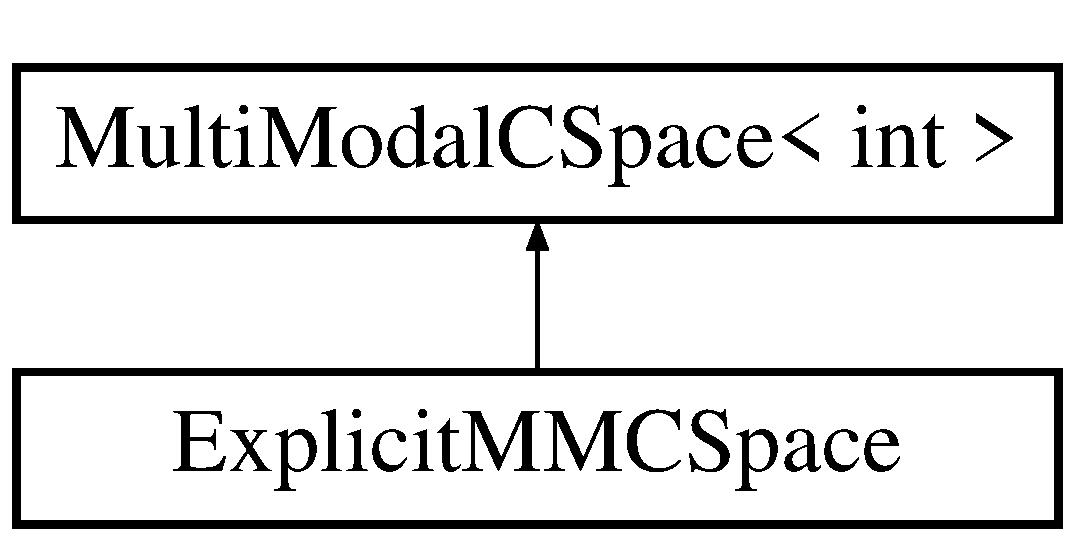
\includegraphics[height=2.000000cm]{classExplicitMMCSpace}
\end{center}
\end{figure}
\subsection*{Public Types}
\begin{DoxyCompactItemize}
\item 
typedef int {\bfseries Mode}\label{classExplicitMMCSpace_a0af02036bb571c63e731688b1d8c403d}

\item 
typedef Graph\+::\+Undirected\+Graph$<$ {\bf C\+Space} $\ast$, {\bf C\+Space} $\ast$ $>$ {\bfseries Mode\+Graph}\label{classExplicitMMCSpace_a091f2eedea51d71cf0ed1e9c2352cd3b}

\end{DoxyCompactItemize}
\subsection*{Public Member Functions}
\begin{DoxyCompactItemize}
\item 
void {\bfseries Delete\+All} ()\label{classExplicitMMCSpace_abbb66e5eabcc9315fa440aebfdb37279}

\item 
virtual bool {\bfseries Is\+Valid} (const Mode \&m)\label{classExplicitMMCSpace_ab86403ad9a528c03d4bef47b96c27af4}

\item 
virtual {\bf C\+Space} $\ast$ {\bfseries Get\+Mode\+C\+Space} (const Mode \&m)\label{classExplicitMMCSpace_a080b76c3e9b6fbbaadf06788e8986dfc}

\item 
virtual {\bf C\+Space} $\ast$ {\bfseries Get\+Transition\+C\+Space} (const Mode \&m1, const Mode \&m2)\label{classExplicitMMCSpace_ab0e5de2a202558fa37166efe63f0081c}

\item 
virtual bool {\bfseries Can\+Enum} () const \label{classExplicitMMCSpace_aa8bc960ae3ce6b41140c07a68f3aed47}

\item 
virtual bool {\bfseries Can\+Sample} () const \label{classExplicitMMCSpace_a6c345ef55469d08c2123ef10d5a9bff4}

\item 
virtual void {\bfseries Enum} (std\+::vector$<$ Mode $>$ \&modes)\label{classExplicitMMCSpace_a9ce70380cf3958b024c0135626e96583}

\item 
virtual void {\bfseries Sample} (std\+::vector$<$ Mode $>$ \&modes)\label{classExplicitMMCSpace_a4431fd733f9704d0e0fb11818b3a0e79}

\item 
virtual bool {\bfseries Can\+Enum\+Adjacent} () const \label{classExplicitMMCSpace_a0e8188bbd57b2f51d4e56a3824fff1d5}

\item 
virtual bool {\bfseries Can\+Sample\+Adjacent} () const \label{classExplicitMMCSpace_ade60ed7e2950f5634c2fb8107984326c}

\item 
virtual bool {\bfseries Can\+Test\+Adjacent} () const \label{classExplicitMMCSpace_a1862c1696fe18a21db710b30aa5d3961}

\item 
virtual void {\bfseries Enum\+Adjacent} (const Mode \&m, std\+::vector$<$ Mode $>$ \&modes)\label{classExplicitMMCSpace_a3c2e277e7ab288bf64e5400b6184c856}

\item 
virtual void {\bfseries Sample\+Adjacent} (const Mode \&m, std\+::vector$<$ Mode $>$ \&adj)\label{classExplicitMMCSpace_a61ea125d818f08914c9e17d5eb7bf605}

\item 
virtual bool {\bfseries Test\+Adjacent} (const Mode \&m1, const Mode \&m2)\label{classExplicitMMCSpace_a9d4cb4887a49a65dacdf516d38790dd8}

\end{DoxyCompactItemize}
\subsection*{Public Attributes}
\begin{DoxyCompactItemize}
\item 
Mode\+Graph {\bfseries mode\+Graph}\label{classExplicitMMCSpace_aa956f78edb24ebee606e88a443a205b3}

\end{DoxyCompactItemize}


The documentation for this class was generated from the following file\+:\begin{DoxyCompactItemize}
\item 
Multi\+Modal\+C\+Space.\+h\end{DoxyCompactItemize}

\section{False\+Edge\+Planner Class Reference}
\label{classFalseEdgePlanner}\index{False\+Edge\+Planner@{False\+Edge\+Planner}}


Edge planner that is never visible.  




{\ttfamily \#include $<$Edge\+Planner.\+h$>$}

Inheritance diagram for False\+Edge\+Planner\+:\begin{figure}[H]
\begin{center}
\leavevmode
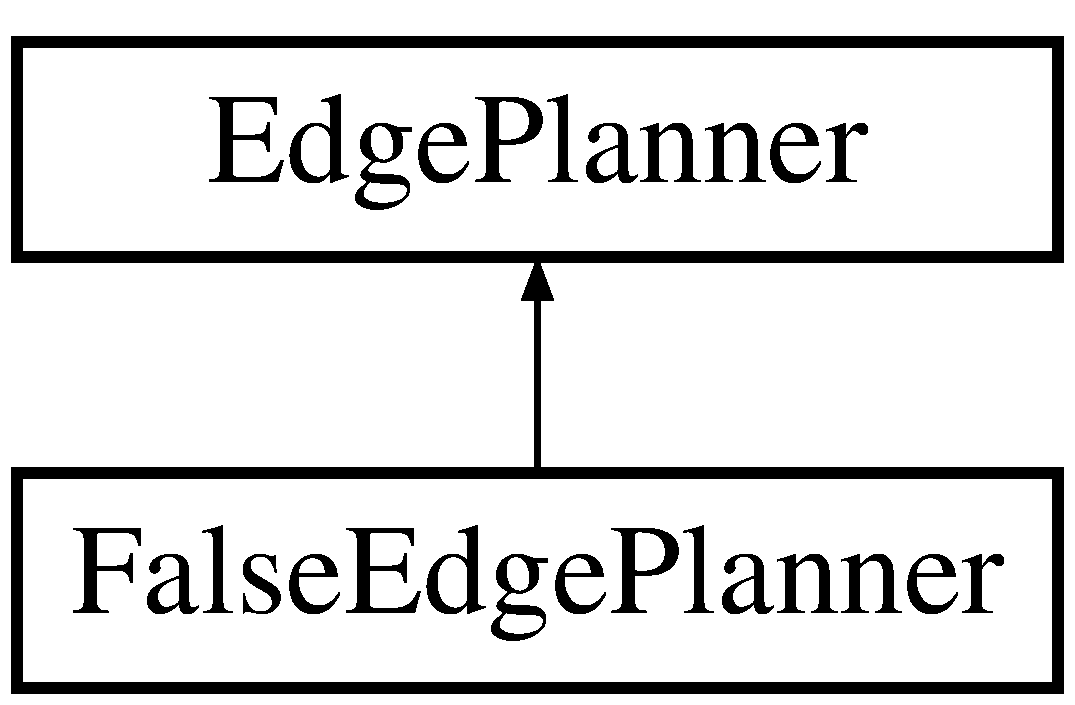
\includegraphics[height=2.000000cm]{classFalseEdgePlanner}
\end{center}
\end{figure}
\subsection*{Public Member Functions}
\begin{DoxyCompactItemize}
\item 
{\bfseries False\+Edge\+Planner} ({\bf C\+Space} $\ast$space, const Config \&x, const Config \&y)\label{classFalseEdgePlanner_ab4372dd7f150d1a45f3f1f924a823392}

\item 
virtual bool {\bfseries Is\+Visible} ()\label{classFalseEdgePlanner_abb7e67a0720697bcade50715c6dc663d}

\item 
virtual void {\bfseries Eval} (double u, Config \&x) const \label{classFalseEdgePlanner_a9da01f9447a410ebada0bf57e34ca51d}

\item 
virtual const Config \& {\bfseries Start} () const \label{classFalseEdgePlanner_a0f230c81b2e01037745a04b90109ce55}

\item 
virtual const Config \& {\bfseries Goal} () const \label{classFalseEdgePlanner_a0eedee8131e9ce77467ecfdb2303f911}

\item 
virtual {\bf C\+Space} $\ast$ {\bfseries Space} () const \label{classFalseEdgePlanner_aac2a49352387d7a02611544a159dabdd}

\item 
virtual {\bf Edge\+Planner} $\ast$ {\bfseries Copy} () const \label{classFalseEdgePlanner_a9ec7ec6d3338aca3cf2245d390216925}

\item 
virtual {\bf Edge\+Planner} $\ast$ {\bfseries Reverse\+Copy} () const \label{classFalseEdgePlanner_adc7f028ecf7f04395939584a01d69806}

\end{DoxyCompactItemize}
\subsection*{Public Attributes}
\begin{DoxyCompactItemize}
\item 
Config {\bfseries a}\label{classFalseEdgePlanner_a862f456b32a8beacee24b16596a3cbb3}

\item 
Config {\bfseries b}\label{classFalseEdgePlanner_ae092fd61b7363c1204a2046bef5d0624}

\item 
{\bf C\+Space} $\ast$ {\bfseries space}\label{classFalseEdgePlanner_abe4989ed73d0d2c81595b571822a0de6}

\end{DoxyCompactItemize}


\subsection{Detailed Description}
Edge planner that is never visible. 

The documentation for this class was generated from the following files\+:\begin{DoxyCompactItemize}
\item 
Edge\+Planner.\+h\item 
Edge\+Planner.\+cpp\end{DoxyCompactItemize}

\section{Greedy\+Subset\+A\+Star Struct Reference}
\label{structGreedySubsetAStar}\index{Greedy\+Subset\+A\+Star@{Greedy\+Subset\+A\+Star}}
Inheritance diagram for Greedy\+Subset\+A\+Star\+:\begin{figure}[H]
\begin{center}
\leavevmode
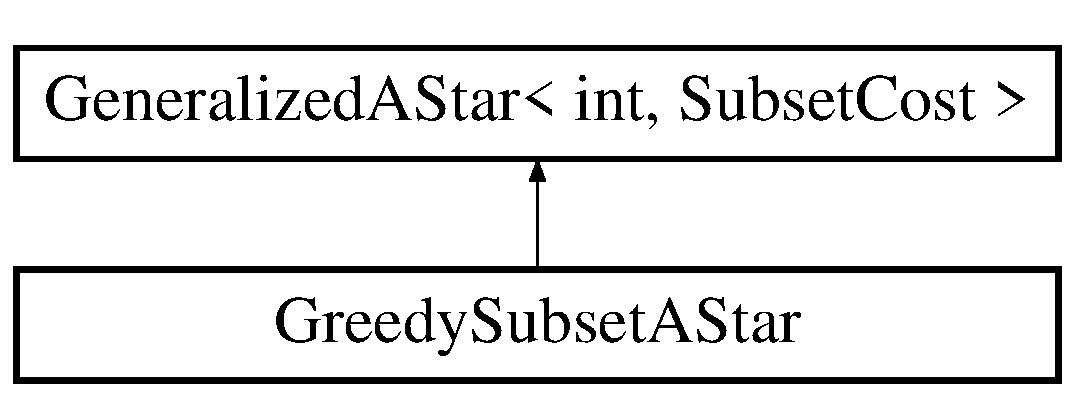
\includegraphics[height=2.000000cm]{structGreedySubsetAStar}
\end{center}
\end{figure}
\subsection*{Public Types}
\begin{DoxyCompactItemize}
\item 
typedef Generalized\+A\+Star$<$ int, {\bf Subset\+Cost} $>$\+::Node {\bfseries Node}\label{structGreedySubsetAStar_aa96ac65adfcc7e041d5a7d9b49d2a08a}

\end{DoxyCompactItemize}
\subsection*{Public Member Functions}
\begin{DoxyCompactItemize}
\item 
{\bfseries Greedy\+Subset\+A\+Star} ({\bf Error\+Explaining\+Planner} $\ast$\+\_\+planner, int \+\_\+start, int \+\_\+target)\label{structGreedySubsetAStar_aa1dc8a9972761c588685ab024bc2dee3}

\item 
virtual bool {\bfseries Is\+Goal} (const int \&s)\label{structGreedySubsetAStar_a2f45fea4ebce83ed921571ff4e542073}

\item 
virtual void {\bfseries Successors} (const int \&s, vector$<$ int $>$ \&successors, vector$<$ {\bf Subset\+Cost} $>$ \&cost)\label{structGreedySubsetAStar_a5d9d5edc72e649d2aa0069b748ed11d5}

\item 
virtual void {\bfseries Clear\+Visited} ()\label{structGreedySubsetAStar_a42096bab60e1f61a164c6c56f315f36a}

\item 
virtual void {\bfseries Visit} (const int \&s, Node $\ast$n)\label{structGreedySubsetAStar_a3248d8712532af4f0161e9db5118bd3c}

\item 
virtual Node $\ast$ {\bfseries Visited\+State\+Node} (const int \&s)\label{structGreedySubsetAStar_a04fa5416bf5ca260ca00f1930f632079}

\end{DoxyCompactItemize}
\subsection*{Public Attributes}
\begin{DoxyCompactItemize}
\item 
{\bf Error\+Explaining\+Planner} $\ast$ {\bfseries planner}\label{structGreedySubsetAStar_a91e00bacccd22a3cbd3a2ad67dc2876b}

\item 
int {\bfseries start\+Node}\label{structGreedySubsetAStar_ab5623e2391b2f65e1a187b4ed5c3387e}

\item 
int {\bfseries target\+Node}\label{structGreedySubsetAStar_aa99f320a6c6ff15a5a1d3186de415638}

\item 
vector$<$ Node $\ast$ $>$ {\bfseries visited}\label{structGreedySubsetAStar_a79b5f2b372b305acfdf38236b2d580b0}

\end{DoxyCompactItemize}


The documentation for this struct was generated from the following file\+:\begin{DoxyCompactItemize}
\item 
Explaining\+Planner.\+cpp\end{DoxyCompactItemize}

\section{Incremental\+M\+M\+P\+R\+M\+\_\+\+Explicit Class Reference}
\label{classIncrementalMMPRM__Explicit}\index{Incremental\+M\+M\+P\+R\+M\+\_\+\+Explicit@{Incremental\+M\+M\+P\+R\+M\+\_\+\+Explicit}}
\subsection*{Public Member Functions}
\begin{DoxyCompactItemize}
\item 
{\bfseries Incremental\+M\+M\+P\+R\+M\+\_\+\+Explicit} ({\bf Explicit\+M\+M\+C\+Space} $\ast$space)\label{classIncrementalMMPRM__Explicit_a975918f1352ddc700399fee959ae9276}

\item 
void {\bfseries Init} ()\label{classIncrementalMMPRM__Explicit_aa912a31c589fae6add6e9d405a7b0f6f}

\item 
void {\bfseries Plan\+More} ()\label{classIncrementalMMPRM__Explicit_a0e39e957cba994fd8fc0b62784f07936}

\item 
bool {\bfseries Done} () const \label{classIncrementalMMPRM__Explicit_a3027af2f3b265c2a0e80eec664ad3693}

\item 
bool {\bfseries Expand\+More} ()\label{classIncrementalMMPRM__Explicit_a3512e4bba5f5689d2992d1acce889ca2}

\item 
void {\bfseries Refine\+More} ()\label{classIncrementalMMPRM__Explicit_a5927f31ea3d4b304418e0776d028a8be}

\item 
virtual int {\bfseries Pick\+Refine\+Count} ()\label{classIncrementalMMPRM__Explicit_a3517b2328a1fb174a1b3e12c2f0591ca}

\end{DoxyCompactItemize}
\subsection*{Public Attributes}
\begin{DoxyCompactItemize}
\item 
{\bf Explicit\+M\+M\+C\+Space} $\ast$ {\bfseries space}\label{classIncrementalMMPRM__Explicit_aaefec825a64431af3d8a6e4422a45467}

\item 
{\bf Multi\+Modal\+P\+RM} {\bfseries mmprm}\label{classIncrementalMMPRM__Explicit_a3db1fb92b108d13df894419954ba7add}

\item 
{\bf Incremental\+M\+M\+P\+R\+M\+\_\+\+Search} {\bfseries search}\label{classIncrementalMMPRM__Explicit_a48a487c7b5380ee259ba9837712f7732}

\item 
int {\bfseries num\+Refine\+Samples\+Per\+Mode}\label{classIncrementalMMPRM__Explicit_a1ec3e16914a24d5f4fe0196ae4cdfb34}

\item 
int {\bfseries num\+Refine\+Samples\+Per\+Old\+Mode}\label{classIncrementalMMPRM__Explicit_a9ddd538bc72f806bdef240197462d65a}

\item 
int {\bfseries num\+Refine\+Samples\+Constant}\label{classIncrementalMMPRM__Explicit_a9768201de09444b7fe6f4c7fc1b6d3e6}

\item 
bool {\bfseries even\+Refinement}\label{classIncrementalMMPRM__Explicit_a2068d1c71b03529bdd7cf87d8c040b0c}

\item 
vector$<$ bool $>$ {\bfseries last\+Refine\+Set}\label{classIncrementalMMPRM__Explicit_a800bfa8ae2b6a8cf7027c3773c53c085}

\item 
int {\bfseries remaining\+Refine\+Samples}\label{classIncrementalMMPRM__Explicit_a107cba3c86a56a026c56cdea36cd6a57}

\item 
int {\bfseries expand\+Phase\+Count}\label{classIncrementalMMPRM__Explicit_a6d4d92740fa775d431b289f4a45630e9}

\item 
int {\bfseries expand\+Step\+Count}\label{classIncrementalMMPRM__Explicit_ab424e880d9824bbe440b7e90196537c1}

\item 
int {\bfseries refine\+Phase\+Count}\label{classIncrementalMMPRM__Explicit_a90a99c84291dd77272a07d765ebb3428}

\item 
int {\bfseries refine\+Step\+Count}\label{classIncrementalMMPRM__Explicit_a9854ae93c3cb6e71fc49e27461866bad}

\end{DoxyCompactItemize}


The documentation for this class was generated from the following files\+:\begin{DoxyCompactItemize}
\item 
Multi\+Modal\+Planner.\+h\item 
Multi\+Modal\+Planner.\+cpp\end{DoxyCompactItemize}

\section{Incremental\+M\+M\+P\+R\+M\+\_\+\+Search Class Reference}
\label{classIncrementalMMPRM__Search}\index{Incremental\+M\+M\+P\+R\+M\+\_\+\+Search@{Incremental\+M\+M\+P\+R\+M\+\_\+\+Search}}
\subsection*{Public Types}
\begin{DoxyCompactItemize}
\item 
typedef Graph\+::\+Undirected\+Graph$<$ int, {\bf Multi\+Modal\+P\+R\+M\+::\+Transition\+Info} $\ast$ $>$ {\bfseries Search\+Graph}\label{classIncrementalMMPRM__Search_a6c843752db20b17e9f7b32f2040c0421}

\item 
typedef Indexed\+Priority\+Queue$<$ int, double $>$ {\bfseries Fringe}\label{classIncrementalMMPRM__Search_a6603b26978f18e2ebf37d040eac284de}

\item 
typedef {\bf Update\+Priority\+S\+PP} {\bfseries Shortest\+Path\+Problem}\label{classIncrementalMMPRM__Search_a86e61c688846150ffcb21408a4201a9a}

\end{DoxyCompactItemize}
\subsection*{Public Member Functions}
\begin{DoxyCompactItemize}
\item 
virtual double {\bfseries Edge\+Length} (int s, int t)\label{classIncrementalMMPRM__Search_a2b1b3c0b95f180c4933a46a9416cc6aa}

\item 
virtual double {\bfseries Edge\+Length} ({\bf Multi\+Modal\+P\+R\+M\+::\+Transition\+Info} $\ast$trans, int s, int t)\label{classIncrementalMMPRM__Search_af60d305062ed653ca312702a15d2cdb2}

\item 
virtual double {\bfseries Heuristic} (int mode)\label{classIncrementalMMPRM__Search_ae27d32ac05bc4dc3b9b6e510be5dcdc3}

\item 
{\bfseries Incremental\+M\+M\+P\+R\+M\+\_\+\+Search} ({\bf Multi\+Modal\+P\+RM} \&mmprm)\label{classIncrementalMMPRM__Search_ad2ab253f2d3002422af5e3187ba4822f}

\item 
void {\bfseries Init} ()\label{classIncrementalMMPRM__Search_ad7d2e7b4b9170945c740c246803918fa}

\item 
bool {\bfseries Expand\+More} ()\label{classIncrementalMMPRM__Search_a9e902b8077113d8255ec54be30492d46}

\item 
void {\bfseries Sample\+More} (int n)\label{classIncrementalMMPRM__Search_a65924b1da473cddf709676687d6499c9}

\item 
void {\bfseries Expand\+Adjacent} (int n)\label{classIncrementalMMPRM__Search_a750b3b2a518bc9f0046c2709a6ff227b}

\item 
void {\bfseries Add\+Edge} (int s, int t, {\bf Multi\+Modal\+P\+R\+M\+::\+Transition\+Info} $\ast$e)\label{classIncrementalMMPRM__Search_a7837e08979f6e1f7e287470f3adebce7}

\item 
void {\bfseries Push\+Fringe} (int i)\label{classIncrementalMMPRM__Search_aaaa2cc88ea58e2a53e109dfd251e2264}

\item 
void {\bfseries Update\+Fringe} (int i)\label{classIncrementalMMPRM__Search_a32686f9ea35015d5e4c4f2b39c3a45d6}

\item 
int {\bfseries Pop\+Fringe} ()\label{classIncrementalMMPRM__Search_a94ef3b155d1542003605d718ed2f447e}

\item 
void {\bfseries Refresh\+Fringe} ()\label{classIncrementalMMPRM__Search_ae11eaf5319351ef6ebaf28e748df234a}

\item 
double {\bfseries Priority} (int n)\label{classIncrementalMMPRM__Search_acfeca387d59f1171f7827022ded4a5ad}

\item 
bool {\bfseries Goal\+Connected} () const \label{classIncrementalMMPRM__Search_a6628b83e7d292c55e816b0a7631cb3dd}

\item 
double {\bfseries Path\+Distance} (int n) const \label{classIncrementalMMPRM__Search_a4d32439292429d217fd1bbf5cf2b63f9}

\item 
void {\bf Update\+Edge\+Length} (int s, int t)\label{classIncrementalMMPRM__Search_adec0489f45770b6ee3155e711eb8965d}

\begin{DoxyCompactList}\small\item\em This must be called when an edge length changes. \end{DoxyCompactList}\item 
void {\bf Update\+Priority} (int n)
\end{DoxyCompactItemize}
\subsection*{Public Attributes}
\begin{DoxyCompactItemize}
\item 
{\bf Multi\+Modal\+P\+RM} \& {\bfseries mmprm}\label{classIncrementalMMPRM__Search_ad4cf73a918dc8c182cb06e09a3787e6e}

\item 
Fringe {\bfseries fringe}\label{classIncrementalMMPRM__Search_afa84f941db578af60730106e137fc0b7}

\item 
{\bf Shortest\+Path\+Problem} {\bfseries spp}\label{classIncrementalMMPRM__Search_a9509786a6874901faacc867513fb5893}

\item 
Search\+Graph {\bfseries search\+Graph}\label{classIncrementalMMPRM__Search_aacf0e12da58b95c61c95414f5c9d225f}

\item 
vector$<$ bool $>$ {\bfseries reached\+Modes}\label{classIncrementalMMPRM__Search_aef3902048d8c2aefa6dc8d3cd1fda20b}

\item 
vector$<$ bool $>$ {\bfseries output\+Modes}\label{classIncrementalMMPRM__Search_adb79539a31e6805a8549ae299e6118c7}

\item 
double {\bfseries trans\+Sample\+Weight}\label{classIncrementalMMPRM__Search_a65b3f5f62c062b8742bc5d9dcb39e567}

\end{DoxyCompactItemize}


\subsection{Member Function Documentation}
\index{Incremental\+M\+M\+P\+R\+M\+\_\+\+Search@{Incremental\+M\+M\+P\+R\+M\+\_\+\+Search}!Update\+Priority@{Update\+Priority}}
\index{Update\+Priority@{Update\+Priority}!Incremental\+M\+M\+P\+R\+M\+\_\+\+Search@{Incremental\+M\+M\+P\+R\+M\+\_\+\+Search}}
\subsubsection[{Update\+Priority(int n)}]{\setlength{\rightskip}{0pt plus 5cm}void Incremental\+M\+M\+P\+R\+M\+\_\+\+Search\+::\+Update\+Priority (
\begin{DoxyParamCaption}
\item[{int}]{n}
\end{DoxyParamCaption}
)}\label{classIncrementalMMPRM__Search_a1a13ee20f33d3c63599ee215ab08ccb7}
This must be called when a heuristic value changes. Called internally in Update\+Edge\+Length. 

The documentation for this class was generated from the following files\+:\begin{DoxyCompactItemize}
\item 
Multi\+Modal\+Planner.\+h\item 
Multi\+Modal\+Planner.\+cpp\end{DoxyCompactItemize}

\section{Int\+Triple Struct Reference}
\label{structIntTriple}\index{Int\+Triple@{Int\+Triple}}
\subsection*{Public Member Functions}
\begin{DoxyCompactItemize}
\item 
bool {\bfseries operator$<$} (const {\bf Int\+Triple} \&t) const \label{structIntTriple_a1080e54d332a15a1f7d742e62efae34c}

\end{DoxyCompactItemize}
\subsection*{Public Attributes}
\begin{DoxyCompactItemize}
\item 
int {\bfseries a}\label{structIntTriple_a5d10312a9920d80760c3d820caca2ce9}

\item 
int {\bfseries b}\label{structIntTriple_a2cf859a35c1e10f8dfa5c293e712a993}

\item 
int {\bfseries c}\label{structIntTriple_ad610e7ea4eed06f3548e34d2af050dbf}

\end{DoxyCompactItemize}


The documentation for this struct was generated from the following file\+:\begin{DoxyCompactItemize}
\item 
Multi\+Modal\+Planner.\+cpp\end{DoxyCompactItemize}

\section{Less\+Edge\+Priority Struct Reference}
\label{structLessEdgePriority}\index{Less\+Edge\+Priority@{Less\+Edge\+Priority}}
\subsection*{Public Types}
\begin{DoxyCompactItemize}
\item 
typedef {\bf S\+B\+L\+Tree\+::\+Edge\+Info} {\bfseries Edge\+Info}\label{structLessEdgePriority_ab1f48c8d7d68ff3fb1f30e4d0c81651c}

\end{DoxyCompactItemize}
\subsection*{Public Member Functions}
\begin{DoxyCompactItemize}
\item 
bool {\bfseries operator()} ({\bf Edge\+Info} \&a, {\bf Edge\+Info} \&b) const \label{structLessEdgePriority_a1cd19fa34c7a01617aef611a2290e09f}

\end{DoxyCompactItemize}


The documentation for this struct was generated from the following file\+:\begin{DoxyCompactItemize}
\item 
S\+B\+L\+Tree.\+cpp\end{DoxyCompactItemize}

\section{Tree\+Roadmap\+Planner\+:\+:Milestone Struct Reference}
\label{structTreeRoadmapPlanner_1_1Milestone}\index{Tree\+Roadmap\+Planner\+::\+Milestone@{Tree\+Roadmap\+Planner\+::\+Milestone}}
\subsection*{Public Attributes}
\begin{DoxyCompactItemize}
\item 
Config {\bfseries x}\label{structTreeRoadmapPlanner_1_1Milestone_ac46bf74c5f8ce2bbccb2d4a5b68b3020}

\item 
int {\bfseries connected\+Component}\label{structTreeRoadmapPlanner_1_1Milestone_a99a7d65ce11b012f4c21a8e584672dea}

\end{DoxyCompactItemize}


The documentation for this struct was generated from the following file\+:\begin{DoxyCompactItemize}
\item 
Motion\+Planner.\+h\end{DoxyCompactItemize}

\section{Error\+Explaining\+Planner\+:\+:Milestone Struct Reference}
\label{structErrorExplainingPlanner_1_1Milestone}\index{Error\+Explaining\+Planner\+::\+Milestone@{Error\+Explaining\+Planner\+::\+Milestone}}
\subsection*{Public Attributes}
\begin{DoxyCompactItemize}
\item 
Config {\bfseries q}\label{structErrorExplainingPlanner_1_1Milestone_abf8488fe8871bebab3ea73ee391349e9}

\item 
int {\bfseries mode}\label{structErrorExplainingPlanner_1_1Milestone_ad98b2047a092ce396b70994db55552a7}

\end{DoxyCompactItemize}


The documentation for this struct was generated from the following file\+:\begin{DoxyCompactItemize}
\item 
Explaining\+Planner.\+h\end{DoxyCompactItemize}

\section{Milestone\+Path Class Reference}
\label{classMilestonePath}\index{Milestone\+Path@{Milestone\+Path}}


A sequence of locally planned paths between milestones.  




{\ttfamily \#include $<$Milestone\+Path.\+h$>$}

\subsection*{Public Member Functions}
\begin{DoxyCompactItemize}
\item 
const Config \& {\bfseries Get\+Milestone} (int milestone) const \label{classMilestonePath_ad6f6f1d1724721b51dd6e4f0e7536215}

\item 
void {\bfseries Set\+Milestone} (int milestone, const Config \&x)\label{classMilestonePath_ab645aac112a001ff7c6f7b331904d6db}

\item 
const Config \& {\bfseries Start} () const \label{classMilestonePath_ad0fcff61f4a50813435349f71a3ccd70}

\item 
const Config \& {\bfseries End} () const \label{classMilestonePath_a0eb4b13b193b60cebe628b113f337173}

\item 
bool {\bf Check\+Set\+Milestone} (int milestone, const Config \&x)
\item 
{\bf C\+Space} $\ast$ {\bfseries Space} (int i=0) const \label{classMilestonePath_aba8f02fd1d95da6cc748523d874680fe}

\item 
int {\bfseries Num\+Milestones} () const \label{classMilestonePath_a4733a8904b3f991d7a84d6a27396a7c7}

\item 
int {\bfseries Num\+Edges} () const \label{classMilestonePath_abe9af85c5270ab5191d7a1019fcf45c1}

\item 
bool {\bfseries Is\+Valid} ()\label{classMilestonePath_ae5b436d6ce379bad4ad930c8e41eef1c}

\item 
double {\bf Length} () const \label{classMilestonePath_a469bcb59f6ea1ad6c5c722120d4f03fa}

\begin{DoxyCompactList}\small\item\em Returns the sum of the distances between milestones. \end{DoxyCompactList}\item 
void {\bf Concat} (const {\bf Milestone\+Path} \&path)\label{classMilestonePath_aa435533ef62a6cec973489a64e338b4c}

\begin{DoxyCompactList}\small\item\em Adds the path onto the end of this one. \end{DoxyCompactList}\item 
void {\bf Create\+Edges\+From\+Milestones} ({\bf C\+Space} $\ast$space, const vector$<$ Config $>$ \&milestones)\label{classMilestonePath_a81b465171be6e10c9c97031e92915593}

\begin{DoxyCompactList}\small\item\em Create the path that connects the milestones in the given workspace. \end{DoxyCompactList}\item 
bool {\bf Initialize\+Edge\+Plans} ()\label{classMilestonePath_a1f3189d474fa330a99a7f3d4a616c04d}

\begin{DoxyCompactList}\small\item\em Checks the feasibility of all edges, returns true if they all succeed. \end{DoxyCompactList}\item 
bool {\bf Is\+Feasible} ()\label{classMilestonePath_a5c05a9bcc0ded11cbefc52f6da31cd05}

\begin{DoxyCompactList}\small\item\em Checks the feasibility of all milestones and edges, returns true if so. \end{DoxyCompactList}\item 
int {\bf Eval} (double t, Config \&c) const 
\item 
int {\bf Shortcut} ()
\item 
int {\bf Reduce} (int num\+Iters)
\item 
void {\bf Splice} (int start, int goal, const {\bf Milestone\+Path} \&path)
\item 
void {\bf Discretize} (double h)
\item 
int {\bf Discretize\+Edge} (int e, double h)\label{classMilestonePath_aaa257fd37945a9d2d51c82453137ae6e}

\begin{DoxyCompactList}\small\item\em Discretizes only the given edge. Returns the number of new segments. \end{DoxyCompactList}\item 
void {\bf Discretize\+Edge} (int e, const vector$<$ double $>$ \&u)\label{classMilestonePath_a4b06ba022f6f48d8b418d0318f3c8282}

\begin{DoxyCompactList}\small\item\em Discretizes the given edge with the specified interpolation. \end{DoxyCompactList}\item 
bool {\bf Load} (istream \&in, {\bf C\+Space} $\ast$space)\label{classMilestonePath_a1b9c83a24c2ca6454e16c97ae62016de}

\begin{DoxyCompactList}\small\item\em Loads the intermediate milestones, and creates the edges from the given space. \end{DoxyCompactList}\item 
bool {\bf Save} (ostream \&out)\label{classMilestonePath_ac65606d8d23d4be900f26cf7e9d7023e}

\begin{DoxyCompactList}\small\item\em Saves the intermediate milestones. \end{DoxyCompactList}\end{DoxyCompactItemize}
\subsection*{Public Attributes}
\begin{DoxyCompactItemize}
\item 
vector$<$ Smart\+Pointer$<$ {\bf Edge\+Planner} $>$ $>$ {\bfseries edges}\label{classMilestonePath_a3940f3bbac7cb31447ad45f0d42cbd3c}

\end{DoxyCompactItemize}


\subsection{Detailed Description}
A sequence of locally planned paths between milestones. 

If n is the number of edges, the milestones are indexed M0...Mn+1, such that edge k goes from Mk to Mk+1. 

\subsection{Member Function Documentation}
\index{Milestone\+Path@{Milestone\+Path}!Check\+Set\+Milestone@{Check\+Set\+Milestone}}
\index{Check\+Set\+Milestone@{Check\+Set\+Milestone}!Milestone\+Path@{Milestone\+Path}}
\subsubsection[{Check\+Set\+Milestone(int milestone, const Config \&x)}]{\setlength{\rightskip}{0pt plus 5cm}bool Milestone\+Path\+::\+Check\+Set\+Milestone (
\begin{DoxyParamCaption}
\item[{int}]{milestone, }
\item[{const Config \&}]{x}
\end{DoxyParamCaption}
)}\label{classMilestonePath_a958207b9f98d6264a918d26470d9ee7c}
Sets the milestone to x only if x and the paths to adjoining milestones are feasible \index{Milestone\+Path@{Milestone\+Path}!Discretize@{Discretize}}
\index{Discretize@{Discretize}!Milestone\+Path@{Milestone\+Path}}
\subsubsection[{Discretize(double h)}]{\setlength{\rightskip}{0pt plus 5cm}void Milestone\+Path\+::\+Discretize (
\begin{DoxyParamCaption}
\item[{double}]{h}
\end{DoxyParamCaption}
)}\label{classMilestonePath_a41823ef8cbc7abaf9272f591ec1c959c}
Discretizes the path such that each edge is no longer than h. Assumes straight-\/line path segments. 

References Discretize\+Edge().

\index{Milestone\+Path@{Milestone\+Path}!Eval@{Eval}}
\index{Eval@{Eval}!Milestone\+Path@{Milestone\+Path}}
\subsubsection[{Eval(double t, Config \&c) const }]{\setlength{\rightskip}{0pt plus 5cm}int Milestone\+Path\+::\+Eval (
\begin{DoxyParamCaption}
\item[{double}]{t, }
\item[{Config \&}]{c}
\end{DoxyParamCaption}
) const}\label{classMilestonePath_ab0ad404882d4ba13a773f1c57e25c953}
Supposing all milestones have equal time spacings, evaluates the point on the path at time t in [0,1]. Returns the edge of time t. \index{Milestone\+Path@{Milestone\+Path}!Reduce@{Reduce}}
\index{Reduce@{Reduce}!Milestone\+Path@{Milestone\+Path}}
\subsubsection[{Reduce(int num\+Iters)}]{\setlength{\rightskip}{0pt plus 5cm}int Milestone\+Path\+::\+Reduce (
\begin{DoxyParamCaption}
\item[{int}]{num\+Iters}
\end{DoxyParamCaption}
)}\label{classMilestonePath_a4894ebfe3f9a6242f08e149dd0dbbcd9}
Tries to shorten the path by connecting random points with a shortcut, for num\+Iters iterations. Returns \# of shortcuts \index{Milestone\+Path@{Milestone\+Path}!Shortcut@{Shortcut}}
\index{Shortcut@{Shortcut}!Milestone\+Path@{Milestone\+Path}}
\subsubsection[{Shortcut()}]{\setlength{\rightskip}{0pt plus 5cm}int Milestone\+Path\+::\+Shortcut (
\begin{DoxyParamCaption}
{}
\end{DoxyParamCaption}
)}\label{classMilestonePath_abdf192c22970e91d33e8e25459062aba}
Tries to shorten the path by connecting subsequent milestones. Returns \# of shortcuts made. \index{Milestone\+Path@{Milestone\+Path}!Splice@{Splice}}
\index{Splice@{Splice}!Milestone\+Path@{Milestone\+Path}}
\subsubsection[{Splice(int start, int goal, const Milestone\+Path \&path)}]{\setlength{\rightskip}{0pt plus 5cm}void Milestone\+Path\+::\+Splice (
\begin{DoxyParamCaption}
\item[{int}]{start, }
\item[{int}]{goal, }
\item[{const {\bf Milestone\+Path} \&}]{path}
\end{DoxyParamCaption}
)}\label{classMilestonePath_aee525a5c149c3fae7a749565a0f2ff74}
Replaces the section of the path between milestones start and goal with a new path. If the index is negative, erases the corresponding start/goal milestones too. 

Referenced by Discretize\+Edge().



The documentation for this class was generated from the following files\+:\begin{DoxyCompactItemize}
\item 
Milestone\+Path.\+h\item 
Milestone\+Path.\+cpp\end{DoxyCompactItemize}

\section{Error\+Explaining\+Planner\+:\+:Mode Struct Reference}
\label{structErrorExplainingPlanner_1_1Mode}\index{Error\+Explaining\+Planner\+::\+Mode@{Error\+Explaining\+Planner\+::\+Mode}}
\subsection*{Public Attributes}
\begin{DoxyCompactItemize}
\item 
{\bf Subset} {\bfseries subset}\label{structErrorExplainingPlanner_1_1Mode_a59867a943e1d0a3078cf5cc437310b11}

\item 
std\+::vector$<$ int $>$ {\bfseries roadmap\+Nodes}\label{structErrorExplainingPlanner_1_1Mode_a04ad8e6a49a3dad51c2d2d1796b14c22}

\item 
std\+::vector$<$ {\bf Subset} $>$ {\bfseries path\+Covers}\label{structErrorExplainingPlanner_1_1Mode_a44b45dfb0750f9398c03052d61f8eb73}

\item 
double {\bfseries min\+Cost}\label{structErrorExplainingPlanner_1_1Mode_a9b273fbfb8ce1228dc9e93640829d5ef}

\end{DoxyCompactItemize}


The documentation for this struct was generated from the following file\+:\begin{DoxyCompactItemize}
\item 
Explaining\+Planner.\+h\end{DoxyCompactItemize}

\section{Multi\+Modal\+P\+RM\+:\+:Mode\+Info Struct Reference}
\label{structMultiModalPRM_1_1ModeInfo}\index{Multi\+Modal\+P\+R\+M\+::\+Mode\+Info@{Multi\+Modal\+P\+R\+M\+::\+Mode\+Info}}
\subsection*{Public Attributes}
\begin{DoxyCompactItemize}
\item 
Smart\+Pointer$<$ {\bf Motion\+Planner\+Interface} $>$ {\bfseries planner}\label{structMultiModalPRM_1_1ModeInfo_aa66d0a3eb673317a855d6546df0dcd1e}

\item 
int {\bfseries sample\+Count}\label{structMultiModalPRM_1_1ModeInfo_afab8abd1d13f2b44d18ece6fe0016617}

\end{DoxyCompactItemize}


The documentation for this struct was generated from the following file\+:\begin{DoxyCompactItemize}
\item 
Multi\+Modal\+Planner.\+h\end{DoxyCompactItemize}

\section{Motion\+Planner\+Factory Class Reference}
\label{classMotionPlannerFactory}\index{Motion\+Planner\+Factory@{Motion\+Planner\+Factory}}


A factory that assists with comparing the motion planners implemented in L\+M\+PL.  




{\ttfamily \#include $<$Any\+Motion\+Planner.\+h$>$}

\subsection*{Public Types}
\begin{DoxyCompactItemize}
\item 
enum {\bfseries Type} \{ \\*
{\bfseries P\+RM}, 
{\bfseries Lazy\+P\+RM}, 
{\bfseries Perturbation\+Tree}, 
{\bfseries E\+ST}, 
\\*
{\bfseries R\+RT}, 
{\bfseries S\+BL}, 
{\bfseries S\+B\+L\+P\+RT}
 \}\label{classMotionPlannerFactory_aace934d88895485fcb7a336aca080aa0}

\end{DoxyCompactItemize}
\subsection*{Public Member Functions}
\begin{DoxyCompactItemize}
\item 
virtual {\bf Motion\+Planner\+Interface} $\ast$ {\bfseries Create} ({\bf C\+Space} $\ast$space)\label{classMotionPlannerFactory_af0812b0ea851a8e211db5d8e42162322}

\end{DoxyCompactItemize}
\subsection*{Public Attributes}
\begin{DoxyCompactItemize}
\item 
Type {\bfseries type}\label{classMotionPlannerFactory_a6ad307019267f032624f0513b2a6f1c6}

\item 
int {\bfseries knn}\label{classMotionPlannerFactory_ad7e7376320a3c0709428f424bb0e09b9}

\item 
double {\bfseries connection\+Threshold}\label{classMotionPlannerFactory_acf69d190d60771443dc34f444d97e343}

\item 
double {\bfseries perturbation\+Radius}\label{classMotionPlannerFactory_aff88ad25ae3d77288e54d476f8191a0d}

\item 
int {\bfseries perturbation\+Iters}\label{classMotionPlannerFactory_a5cdbd7157b821acf5d4929547ee26c25}

\item 
bool {\bfseries bidirectional}\label{classMotionPlannerFactory_ab0b99e97d45a0f36fe14e6397edecd06}

\item 
bool {\bfseries use\+Grid}\label{classMotionPlannerFactory_a2c31746c308b317ceceee1efa712c761}

\item 
double {\bfseries grid\+Resolution}\label{classMotionPlannerFactory_a67a88644f3a4275d3e47ec5eeaefb6b3}

\item 
int {\bfseries randomize\+Frequency}\label{classMotionPlannerFactory_aead599a7bb7a86231e68d2bd94ce54a7}

\end{DoxyCompactItemize}


\subsection{Detailed Description}
A factory that assists with comparing the motion planners implemented in L\+M\+PL. 

So far, only P\+RM, S\+BL, and \doxyref{S\+B\+L\+P\+RT}{p.}{classSBLPRT} are functional. More will come over time.

Planner settings can be tweaked by changing the members of this class from their default settings. 

The documentation for this class was generated from the following files\+:\begin{DoxyCompactItemize}
\item 
Any\+Motion\+Planner.\+h\item 
Any\+Motion\+Planner.\+cpp\end{DoxyCompactItemize}

\section{Motion\+Planner\+Interface Class Reference}
\label{classMotionPlannerInterface}\index{Motion\+Planner\+Interface@{Motion\+Planner\+Interface}}


A base class for a generic motion planner, which can be used to compare multiple planning algorithms under a common interface.  




{\ttfamily \#include $<$Any\+Motion\+Planner.\+h$>$}

Inheritance diagram for Motion\+Planner\+Interface\+:\begin{figure}[H]
\begin{center}
\leavevmode
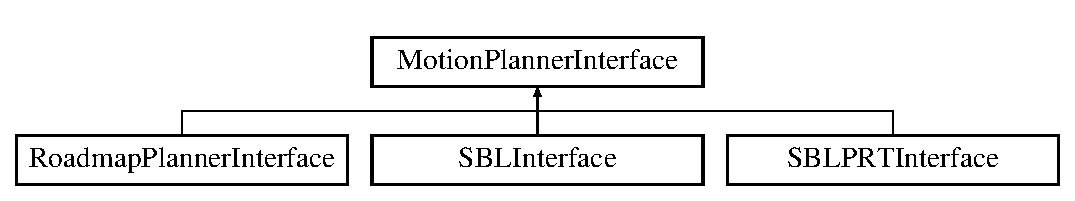
\includegraphics[height=2.000000cm]{classMotionPlannerInterface}
\end{center}
\end{figure}
\subsection*{Public Member Functions}
\begin{DoxyCompactItemize}
\item 
virtual int {\bfseries Plan\+More} ()=0\label{classMotionPlannerInterface_a81be8094ff8ecc8f070178b0ab13943a}

\item 
virtual void {\bfseries Plan\+More} (int num\+Iters)\label{classMotionPlannerInterface_ab15dedf8e15dd82eed4c185067f3d453}

\item 
virtual int {\bfseries Num\+Iterations} () const =0\label{classMotionPlannerInterface_a299bde5aa905aeea95aa34f6210571ae}

\item 
virtual int {\bfseries Num\+Milestones} () const =0\label{classMotionPlannerInterface_a6836d6cb657f841131727780fc0a96b8}

\item 
virtual int {\bfseries Num\+Components} () const =0\label{classMotionPlannerInterface_afb78c259e3402dfb61db41f519f2c7db}

\item 
virtual bool {\bfseries Can\+Add\+Milestone} () const \label{classMotionPlannerInterface_afd0a92e08a1c3832e0d9cf2757d097f2}

\item 
virtual int {\bfseries Add\+Milestone} (const Config \&q)=0\label{classMotionPlannerInterface_a9507063decfc0ea0b89a8f42f562cf0f}

\item 
virtual void {\bfseries Get\+Milestone} (int, Config \&q)=0\label{classMotionPlannerInterface_a4e397f7d21cd7435e1feefa4934c05e4}

\item 
virtual void {\bfseries Connect\+Hint} (int m)\label{classMotionPlannerInterface_a18aea6c99e377f4e7e0dc408e3a6f6d7}

\item 
virtual bool {\bfseries Connect\+Hint} (int ma, int mb)\label{classMotionPlannerInterface_a74fc89bf89add178023d5356bcc68a7f}

\item 
virtual bool {\bfseries Is\+Connected} (int ma, int mb) const =0\label{classMotionPlannerInterface_ab868c9e00e603327d4d64ea52ab66162}

\item 
virtual bool {\bfseries Is\+Lazy} () const \label{classMotionPlannerInterface_ab9642dbf258c803357705592a74e1682}

\item 
virtual bool {\bfseries Check\+Path} (int ma, int mb)\label{classMotionPlannerInterface_a0b41ad29de6a0b40cc7366debad6033b}

\item 
virtual bool {\bfseries Is\+Lazy\+Connected} (int ma, int mb) const \label{classMotionPlannerInterface_abc2b3eef0c54453efcce0772b3dbae2e}

\item 
virtual void {\bfseries Get\+Path} (int ma, int mb, {\bf Milestone\+Path} \&path)=0\label{classMotionPlannerInterface_a4a56cbf7b39e78efaac721d042771d22}

\item 
virtual void {\bfseries Get\+Roadmap} ({\bf Roadmap\+Planner} \&roadmap)\label{classMotionPlannerInterface_adf19b2ff0687d9c3cb00938506ad54e5}

\end{DoxyCompactItemize}


\subsection{Detailed Description}
A base class for a generic motion planner, which can be used to compare multiple planning algorithms under a common interface. 

The documentation for this class was generated from the following file\+:\begin{DoxyCompactItemize}
\item 
Any\+Motion\+Planner.\+h\end{DoxyCompactItemize}

\section{Multi\+Modal\+C\+Space$<$ Mode $>$ Class Template Reference}
\label{classMultiModalCSpace}\index{Multi\+Modal\+C\+Space$<$ Mode $>$@{Multi\+Modal\+C\+Space$<$ Mode $>$}}


Multi-\/modal configuration space base class.  




{\ttfamily \#include $<$Multi\+Modal\+C\+Space.\+h$>$}

\subsection*{Public Member Functions}
\begin{DoxyCompactItemize}
\item 
virtual bool {\bfseries Is\+Valid} (const Mode \&m)\label{classMultiModalCSpace_a3561c41946430ee91d083b1c05981070}

\item 
virtual {\bf C\+Space} $\ast$ {\bfseries Get\+Mode\+C\+Space} (const Mode \&m)\label{classMultiModalCSpace_a72dda3a8af9efc6e1142610eaf1581bc}

\item 
virtual {\bf C\+Space} $\ast$ {\bfseries Get\+Transition\+C\+Space} (const Mode \&m1, const Mode \&m2)\label{classMultiModalCSpace_ab9beb6a054b6ede81f1179ffc72b655f}

\item 
virtual bool {\bfseries Can\+Enum} () const \label{classMultiModalCSpace_abe7479b346e4a8b06cfcb6e107ce508b}

\item 
virtual bool {\bfseries Can\+Sample} () const \label{classMultiModalCSpace_a25329535062243e2baa18679358488a7}

\item 
virtual void {\bfseries Enum} (std\+::vector$<$ Mode $>$ \&modes)\label{classMultiModalCSpace_a99d2ed75fef865d8bc20a9962be84419}

\item 
virtual void {\bfseries Sample} (std\+::vector$<$ Mode $>$ \&modes)\label{classMultiModalCSpace_a500d0af7b023c6f12b2f338fb76feccf}

\item 
virtual bool {\bfseries Can\+Enum\+Adjacent} () const \label{classMultiModalCSpace_af12f75f40a87e2f6fe3db59ce04af304}

\item 
virtual bool {\bfseries Can\+Sample\+Adjacent} () const \label{classMultiModalCSpace_a8ed6f4db485f742d74ce5c94b86dcba1}

\item 
virtual bool {\bfseries Can\+Test\+Adjacent} () const \label{classMultiModalCSpace_a6976171354328312163b25a5d70d195c}

\item 
virtual void {\bfseries Enum\+Adjacent} (const Mode \&m, std\+::vector$<$ Mode $>$ \&modes)\label{classMultiModalCSpace_a7120c6e89f0da1460bd2fb0d77b0e906}

\item 
virtual void {\bfseries Sample\+Adjacent} (const Mode \&m, std\+::vector$<$ Mode $>$ \&adj)\label{classMultiModalCSpace_a074e27ededced39760d32df0595a2ba6}

\item 
virtual bool {\bfseries Test\+Adjacent} (const Mode \&m1, const Mode \&m2)\label{classMultiModalCSpace_a91a5f6af00329a5b57b44a19692b4404}

\end{DoxyCompactItemize}


\subsection{Detailed Description}
\subsubsection*{template$<$class Mode$>$\\*
class Multi\+Modal\+C\+Space$<$ Mode $>$}

Multi-\/modal configuration space base class. 

The class must define the mapping from Modes to C\+Spaces, as well as the C\+Spaces defining the transition region for each pair of adjacent modes. They also describe methods that will allow planners to traverse the mode graph.

There are three types of mode graphs that can be implemented\+: 1) discrete and small, 2) discrete and large, or 3) continuous. The implementations of these types takes on different forms. (Note that representations 2 and 3 are not yet exploited by any planner implemented in L\+M\+PL, but we plan to include support shortly)

For discrete and small mode graphs, the easiest implementation is to explicitly represent the mode graph using the \doxyref{Explicit\+M\+M\+C\+Space}{p.}{classExplicitMMCSpace} class. In this class, you simply fill out the mode\+Graph structure with the correct \doxyref{C\+Space}{p.}{classCSpace}\textquotesingle{}s along its nodes and edges, and all the rest is done.

For discrete and large mode graphs, the graph will be represented implicitly in a search-\/like framework. Subclasses should overload the Can\+Enum\+Adjacent method such that it returns true. They should also implement the Enum\+Adjacent method to return all modes adjacent to the given mode m.

For continuous mode graphs, the graph will be represented by sampling. Subclasses should overload the Can\+Sample\+Adjacent method such that it returns true. They should also implement the Sample\+Adjacent method to sample a set of modes that are adjacent to the given mode m.

The Enum and Sample routines are here for possible future implementations of multi modal planners. 

The documentation for this class was generated from the following file\+:\begin{DoxyCompactItemize}
\item 
Multi\+Modal\+C\+Space.\+h\end{DoxyCompactItemize}

\section{Multi\+Modal\+P\+RM Class Reference}
\label{classMultiModalPRM}\index{Multi\+Modal\+P\+RM@{Multi\+Modal\+P\+RM}}
\subsection*{Classes}
\begin{DoxyCompactItemize}
\item 
struct {\bf Mode\+Info}
\item 
struct {\bf Transition\+Index}
\item 
struct {\bf Transition\+Info}
\end{DoxyCompactItemize}
\subsection*{Public Types}
\begin{DoxyCompactItemize}
\item 
typedef Graph\+::\+Undirected\+Graph$<$ {\bf Mode\+Info}, {\bf Transition\+Info} $>$ {\bfseries Planning\+Graph}\label{classMultiModalPRM_ab20dcf0c96259018f5140f9aaf90af40}

\end{DoxyCompactItemize}
\subsection*{Public Member Functions}
\begin{DoxyCompactItemize}
\item 
{\bfseries Multi\+Modal\+P\+RM} ({\bf Multi\+Modal\+C\+Space}$<$ int $>$ $\ast$cspace)\label{classMultiModalPRM_ad7c8af1d3a9b140e536c86a8bd890ce2}

\item 
void {\bfseries Initialize\+Explicit} ({\bf Explicit\+M\+M\+C\+Space} $\ast$cspace)\label{classMultiModalPRM_af232aa301b1553ac5d55d45a8fa53cdd}

\item 
void {\bfseries Set\+Start} (const Config \&q, int mode)\label{classMultiModalPRM_ae917615f8db03b36ff0ddaf0f964f166}

\item 
void {\bfseries Set\+Goal} (const Config \&q, int mode)\label{classMultiModalPRM_ae7ffa283baaf65dfeb2c16303d88bd49}

\item 
void {\bfseries Set\+Start\+Mode} (int mode)\label{classMultiModalPRM_aa2ac38f9a24e2a4ea73a72ff5124c368}

\item 
void {\bfseries Set\+Goal\+Mode} (int mode)\label{classMultiModalPRM_ac6e6ccf39c5a65bd00bfe326afe6257e}

\item 
void {\bfseries Expand\+All} ()\label{classMultiModalPRM_a36eb6616c195ad84cad95156971dd545}

\item 
void {\bfseries Expand\+Mode} (int mode, int num\+Samples=-\/1)\label{classMultiModalPRM_aedba8361116eef62b1b290cda6d65449}

\item 
void {\bfseries Expand\+Trans} (int m1, int m2, int num\+Samples=-\/1)\label{classMultiModalPRM_a005a73658d3376717d7a6b8f00206753}

\item 
void {\bfseries Add\+Transition} (int m1, int m2, const Config \&q)\label{classMultiModalPRM_a2a76e8aeedd93c71123d3ea0724712e4}

\item 
bool {\bfseries Is\+Start\+And\+Goal\+Connected} () const \label{classMultiModalPRM_ad41e4fa835cf73a304d67229594566ac}

\item 
{\bf Transition\+Index} {\bfseries Node\+To\+Transition\+Index} (int mode, int roadmap\+Index) const \label{classMultiModalPRM_a1d3f9cf5ea83f42f99b5bac2e8167739}

\item 
void {\bfseries Connect\+Transitions} (int mode, int t1, int t2)\label{classMultiModalPRM_a6893a8da2b46d5f5ec39bdece0c85f1c}

\item 
void {\bfseries Connect\+Transitions} (const {\bf Transition\+Index} \&t1, const {\bf Transition\+Index} \&t2)\label{classMultiModalPRM_aa7a9de1acd05cc017c38ad944ecafe17}

\item 
void {\bfseries Get\+Transition\+Nodes} (int mode, vector$<$ {\bf Transition\+Index} $>$ \&transitions, vector$<$ int $>$ \&roadmap\+Indices) const \label{classMultiModalPRM_ad8d72c9a63b95146d9319f900e02675b}

\end{DoxyCompactItemize}
\subsection*{Public Attributes}
\begin{DoxyCompactItemize}
\item 
{\bf Multi\+Modal\+C\+Space}$<$ int $>$ $\ast$ {\bfseries space}\label{classMultiModalPRM_a8bb45b62a40d65d52b11af7b50725fee}

\item 
Planning\+Graph {\bfseries planning\+Graph}\label{classMultiModalPRM_a596e8de91e43ce2dddeb832702adb25e}

\item 
int {\bfseries start\+Mode}\label{classMultiModalPRM_abd565117f0ab56def1adbc0d0b0b7364}

\item 
int {\bfseries start\+Roadmap\+Index}\label{classMultiModalPRM_aec65614f66a1bdf20a375611d9894fed}

\item 
int {\bfseries goal\+Mode}\label{classMultiModalPRM_ae82bc5ee4f4cd22ac7884d03cc763b24}

\item 
int {\bfseries goal\+Roadmap\+Index}\label{classMultiModalPRM_ac4edcaeb7b9f831fb8fb80a7a7d5dc0e}

\item 
int {\bfseries num\+Expand\+Mode\+Samples}\label{classMultiModalPRM_aafcc7e72a29414eccc1a363a39a6df74}

\item 
int {\bfseries num\+Expand\+Trans\+Samples}\label{classMultiModalPRM_a124090370e3e8b159d11683a1ef3e183}

\item 
{\bf Motion\+Planner\+Factory} {\bfseries planner\+Factory}\label{classMultiModalPRM_ac235efba7a0f24aac67c600ffcc6f0db}

\item 
std\+::map$<$ {\bf Transition\+Index}, int $>$ {\bfseries cc\+Index}\label{classMultiModalPRM_a9c3bc4d44c76226d486bafd2f42ce2b8}

\item 
Graph\+::\+Connected\+Components {\bfseries ccs}\label{classMultiModalPRM_a48a2376a9dfcbf9501a7abe54f9e8f58}

\item 
int {\bfseries mode\+Sample\+Count}\label{classMultiModalPRM_ae0d5c25df1c5abe5604e2f67668d9a0d}

\item 
int {\bfseries trans\+Sample\+Count}\label{classMultiModalPRM_ac0f6973bad3547267b393bdacf1a0836}

\end{DoxyCompactItemize}


The documentation for this class was generated from the following files\+:\begin{DoxyCompactItemize}
\item 
Multi\+Modal\+Planner.\+h\item 
Multi\+Modal\+Planner.\+cpp\end{DoxyCompactItemize}

\section{Optimal\+Subset\+A\+Star Struct Reference}
\label{structOptimalSubsetAStar}\index{Optimal\+Subset\+A\+Star@{Optimal\+Subset\+A\+Star}}
Inheritance diagram for Optimal\+Subset\+A\+Star\+:\begin{figure}[H]
\begin{center}
\leavevmode
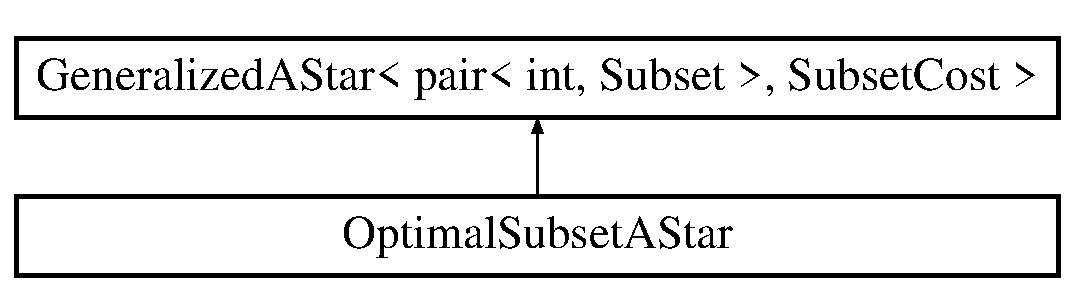
\includegraphics[height=2.000000cm]{structOptimalSubsetAStar}
\end{center}
\end{figure}
\subsection*{Public Types}
\begin{DoxyCompactItemize}
\item 
typedef pair$<$ int, {\bf Subset} $>$ {\bfseries State}\label{structOptimalSubsetAStar_a5e7da724c886144bbf47e2870eb42dff}

\item 
typedef Generalized\+A\+Star$<$ State, {\bf Subset\+Cost} $>$\+::Node {\bfseries Node}\label{structOptimalSubsetAStar_a796b87b95ae65f83786e494d189d217d}

\end{DoxyCompactItemize}
\subsection*{Public Member Functions}
\begin{DoxyCompactItemize}
\item 
{\bfseries Optimal\+Subset\+A\+Star} ({\bf Error\+Explaining\+Planner} $\ast$\+\_\+planner, int \+\_\+start, int \+\_\+target)\label{structOptimalSubsetAStar_afd6df9310a118c2fcb90b58a53fc1f9f}

\item 
virtual bool {\bfseries Is\+Goal} (const State \&s)\label{structOptimalSubsetAStar_a8b6a6fb65356d468293218231bb97c26}

\item 
virtual void {\bfseries Successors} (const State \&s, vector$<$ State $>$ \&successors, vector$<$ {\bf Subset\+Cost} $>$ \&cost)\label{structOptimalSubsetAStar_a4538406b36aaa88f5263d659aa8ee293}

\item 
virtual void {\bfseries Clear\+Visited} ()\label{structOptimalSubsetAStar_a680ff03bd25a991834a44ca301045305}

\item 
virtual void {\bfseries Visit} (const State \&s, Node $\ast$n)\label{structOptimalSubsetAStar_a724d3445f40d0a6e1986137b4bc2ca51}

\item 
virtual Node $\ast$ {\bfseries Visited\+State\+Node} (const State \&s)\label{structOptimalSubsetAStar_a9f526192902fd48d57c0de1662727116}

\end{DoxyCompactItemize}
\subsection*{Public Attributes}
\begin{DoxyCompactItemize}
\item 
{\bf Error\+Explaining\+Planner} $\ast$ {\bfseries planner}\label{structOptimalSubsetAStar_a5bb51a35a94f0af9c266139c687fdf4e}

\item 
int {\bfseries start\+Node}\label{structOptimalSubsetAStar_ac7871f90cd6594a08b7667a1579b2908}

\item 
int {\bfseries target\+Node}\label{structOptimalSubsetAStar_a36443ceb5144056c4dacbc7bb4f6eb46}

\item 
vector$<$ vector$<$ pair$<$ {\bf Subset}, Node $\ast$ $>$ $>$ $>$ {\bfseries visited}\label{structOptimalSubsetAStar_a1558e620e3187a163f2389684efafa81}

\end{DoxyCompactItemize}


The documentation for this struct was generated from the following file\+:\begin{DoxyCompactItemize}
\item 
Explaining\+Planner.\+cpp\end{DoxyCompactItemize}

\section{Path\+Info Struct Reference}
\label{structPathInfo}\index{Path\+Info@{Path\+Info}}
\subsection*{Public Attributes}
\begin{DoxyCompactItemize}
\item 
int {\bfseries tstart}\label{structPathInfo_a8079a96654eb2ef34e0e2a7cfc2ea6f6}

\item 
int {\bfseries tgoal}\label{structPathInfo_a8bb21e9023ab59f4e0f6daa9b06decb5}

\item 
{\bf Milestone\+Path} $\ast$ {\bfseries path}\label{structPathInfo_a4db317950c2af94aafe08e234570c4e3}

\end{DoxyCompactItemize}


The documentation for this struct was generated from the following file\+:\begin{DoxyCompactItemize}
\item 
S\+B\+L.\+cpp\end{DoxyCompactItemize}

\section{Perturbation\+Tree\+Planner Class Reference}
\label{classPerturbationTreePlanner}\index{Perturbation\+Tree\+Planner@{Perturbation\+Tree\+Planner}}


A tree-\/based randomized planner that extends the roadmap by sampling the neighborhood of existing samples.  




{\ttfamily \#include $<$Motion\+Planner.\+h$>$}

Inheritance diagram for Perturbation\+Tree\+Planner\+:\begin{figure}[H]
\begin{center}
\leavevmode
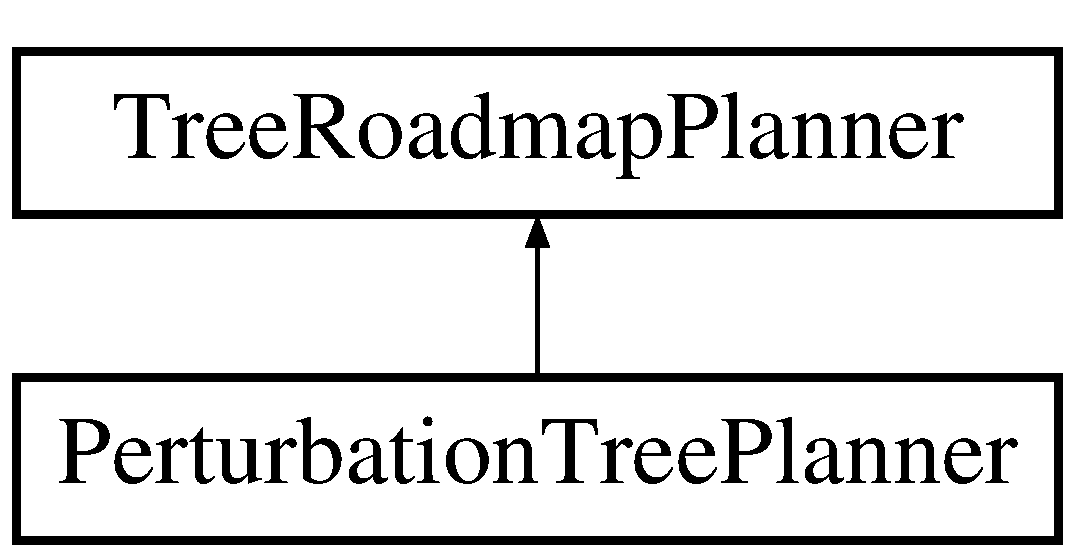
\includegraphics[height=2.000000cm]{classPerturbationTreePlanner}
\end{center}
\end{figure}
\subsection*{Public Member Functions}
\begin{DoxyCompactItemize}
\item 
{\bfseries Perturbation\+Tree\+Planner} ({\bf C\+Space} $\ast$s)\label{classPerturbationTreePlanner_a099fa6cd4b3ba628254cf6e078d08dc2}

\item 
virtual void {\bfseries Generate\+Config} (Config \&x)\label{classPerturbationTreePlanner_a61284d3fb56cd90321747a2930bf9805}

\item 
virtual Node $\ast$ {\bfseries Add\+Feasible\+Milestone} (const Config \&x)\label{classPerturbationTreePlanner_adf7f83d9404e5558d479c80cf5270d63}

\item 
virtual void {\bfseries Cleanup} ()\label{classPerturbationTreePlanner_a0d39b8652c4a87cd8a6d93956f292378}

\item 
virtual Node $\ast$ {\bfseries Select\+Milestone} (const std\+::vector$<$ Node $\ast$ $>$ \&milestones)\label{classPerturbationTreePlanner_aaede55096272a619a11a0de1e175e496}

\end{DoxyCompactItemize}
\subsection*{Public Attributes}
\begin{DoxyCompactItemize}
\item 
double {\bf delta}\label{classPerturbationTreePlanner_a515688424c6bf53a9f5a77952091c326}

\begin{DoxyCompactList}\small\item\em Neighborhood distance. \end{DoxyCompactList}\item 
std\+::vector$<$ double $>$ {\bf weights}\label{classPerturbationTreePlanner_abfe29d343ea150e30a3d28218b542391}

\begin{DoxyCompactList}\small\item\em Node selection weights. \end{DoxyCompactList}\end{DoxyCompactItemize}
\subsection*{Additional Inherited Members}


\subsection{Detailed Description}
A tree-\/based randomized planner that extends the roadmap by sampling the neighborhood of existing samples. 

The existing sample picked is selected with probability proportional to its value in the weight vector. By default, a new node is given weight 1.

The E\+ST planner can be implemented on top of this planner by setting appropriate weights. This functionality is not yet implemented. 

The documentation for this class was generated from the following files\+:\begin{DoxyCompactItemize}
\item 
Motion\+Planner.\+h\item 
Motion\+Planner.\+cpp\end{DoxyCompactItemize}

\section{Pick\+Callback Struct Reference}
\label{structPickCallback}\index{Pick\+Callback@{Pick\+Callback}}
Inheritance diagram for Pick\+Callback\+:\begin{figure}[H]
\begin{center}
\leavevmode
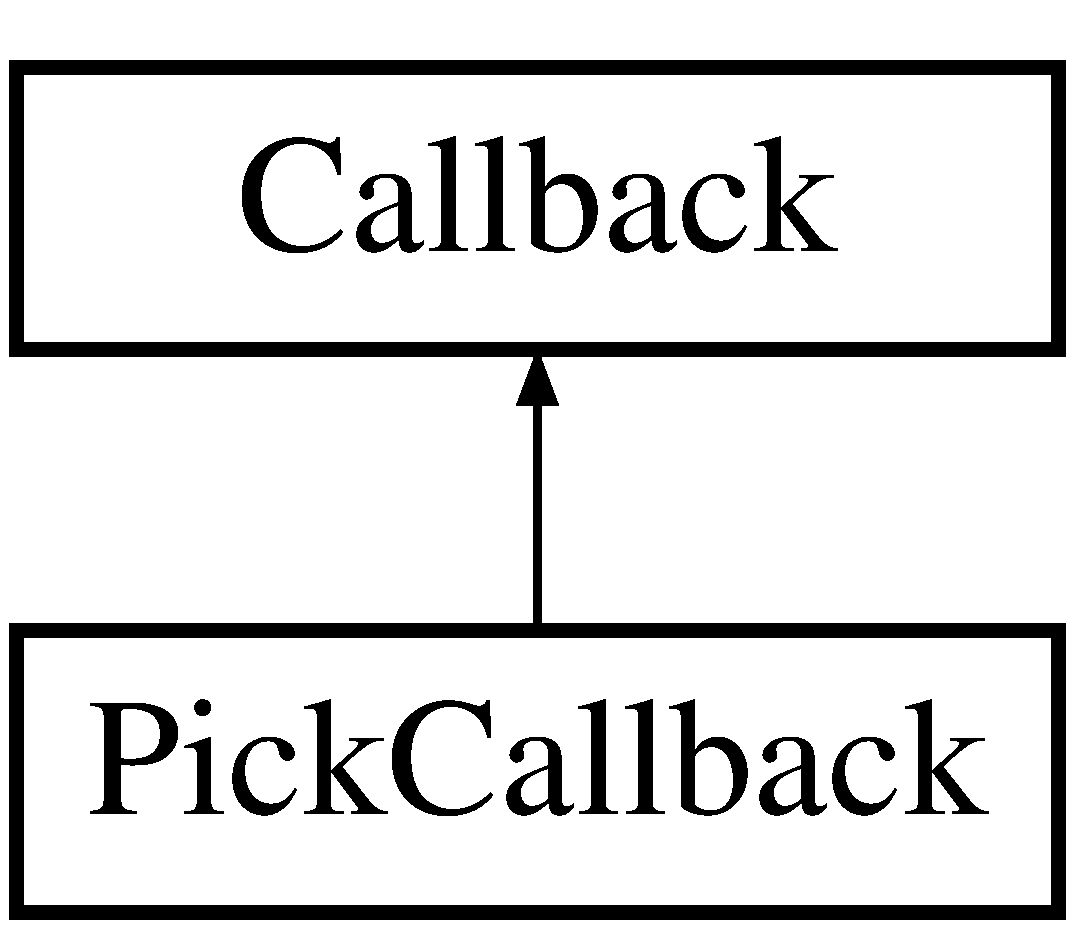
\includegraphics[height=2.000000cm]{structPickCallback}
\end{center}
\end{figure}
\subsection*{Public Member Functions}
\begin{DoxyCompactItemize}
\item 
{\bfseries Pick\+Callback} (int \+\_\+k)\label{structPickCallback_af50fca53a56421d636f3d9b3a5de31cf}

\item 
virtual void {\bfseries Visit} (Node $\ast$n)\label{structPickCallback_a8f88f99820d6dd469fc6c8f97f14bfc7}

\item 
virtual bool {\bfseries Stop} ()\label{structPickCallback_a71d8b7e130a62cf53abd8d3d08f7d784}

\end{DoxyCompactItemize}
\subsection*{Public Attributes}
\begin{DoxyCompactItemize}
\item 
int {\bfseries i}\label{structPickCallback_aeb2d83f851d851183c61f85eb7392f9b}

\item 
int {\bfseries k}\label{structPickCallback_a38f80e9d72a8f2f47830088d15ea2d12}

\item 
Node $\ast$ {\bfseries res}\label{structPickCallback_a25ec700b1ce1a91c7912469afd08206a}

\end{DoxyCompactItemize}


The documentation for this struct was generated from the following file\+:\begin{DoxyCompactItemize}
\item 
S\+B\+L\+Tree.\+cpp\end{DoxyCompactItemize}

\section{Piggyback\+Edge\+Planner Class Reference}
\label{classPiggybackEdgePlanner}\index{Piggyback\+Edge\+Planner@{Piggyback\+Edge\+Planner}}


{\ttfamily \#include $<$Edge\+Planner.\+h$>$}

Inheritance diagram for Piggyback\+Edge\+Planner\+:\begin{figure}[H]
\begin{center}
\leavevmode
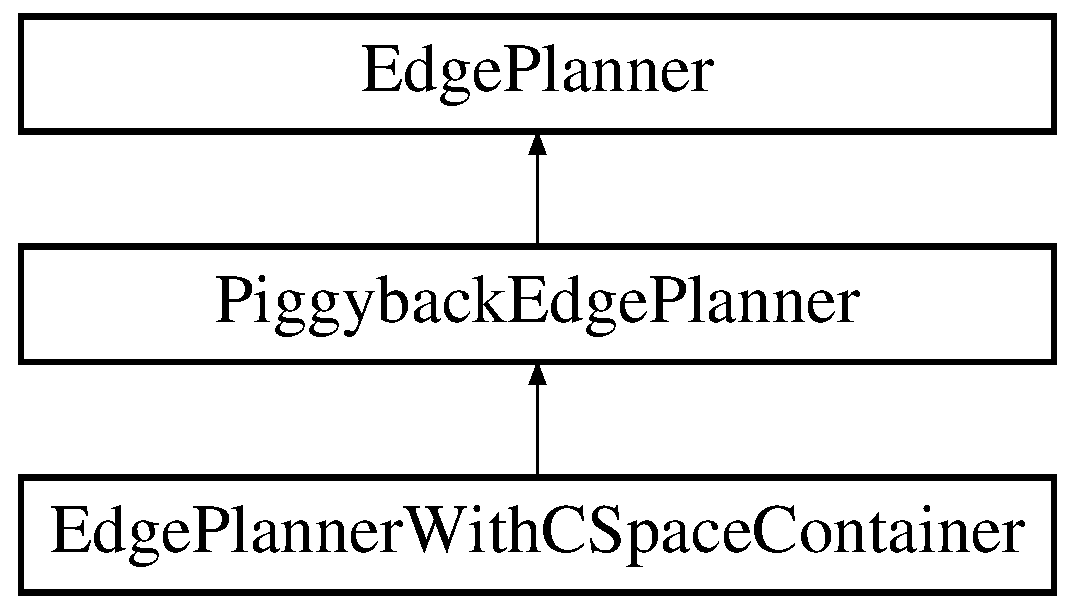
\includegraphics[height=3.000000cm]{classPiggybackEdgePlanner}
\end{center}
\end{figure}
\subsection*{Public Member Functions}
\begin{DoxyCompactItemize}
\item 
{\bfseries Piggyback\+Edge\+Planner} ({\bf C\+Space} $\ast$space, const Config \&a, const Config \&b, const Smart\+Pointer$<$ {\bf Edge\+Planner} $>$ \&e)\label{classPiggybackEdgePlanner_a8a7a0e442d566f471261f38f6c0b0ca7}

\item 
virtual bool {\bfseries Is\+Visible} ()\label{classPiggybackEdgePlanner_a29531b1409f23b9395f56ed7b3975deb}

\item 
virtual void {\bfseries Eval} (double u, Config \&x) const \label{classPiggybackEdgePlanner_a1b58547f0f4d4120f5a7b10ab65343c3}

\item 
virtual const Config \& {\bfseries Start} () const \label{classPiggybackEdgePlanner_a6f8e2b0637ee39fc46c25f2155628a21}

\item 
virtual const Config \& {\bfseries Goal} () const \label{classPiggybackEdgePlanner_abaf504e2b9aea8436edce876f169e358}

\item 
virtual {\bf C\+Space} $\ast$ {\bfseries Space} () const \label{classPiggybackEdgePlanner_a78922318d9668757c3fc31a75fe4793f}

\item 
virtual {\bf Edge\+Planner} $\ast$ {\bfseries Copy} () const \label{classPiggybackEdgePlanner_afa82124bc879db5bf5fb9313ce987b6c}

\item 
virtual {\bf Edge\+Planner} $\ast$ {\bfseries Reverse\+Copy} () const \label{classPiggybackEdgePlanner_a50453ad3d6b4ce6f2ac641f6ed5c20cd}

\item 
virtual double {\bfseries Priority} () const \label{classPiggybackEdgePlanner_a5b30aead46b654cd64080f288d96abc1}

\item 
virtual bool {\bfseries Plan} ()\label{classPiggybackEdgePlanner_a6b60eb41d119a0944401369be2c148f1}

\item 
virtual bool {\bfseries Done} () const \label{classPiggybackEdgePlanner_a550a9d05d08979531cbbc42cf43c6fd4}

\item 
virtual bool {\bfseries Failed} () const \label{classPiggybackEdgePlanner_ab16faca26566c9d4038cf586089ec6a7}

\end{DoxyCompactItemize}
\subsection*{Public Attributes}
\begin{DoxyCompactItemize}
\item 
Config {\bfseries a}\label{classPiggybackEdgePlanner_a4c28f1ae75632a7a769c366ce9bd8594}

\item 
Config {\bfseries b}\label{classPiggybackEdgePlanner_a57d6166f6d0d62234940d83fe4c30553}

\item 
{\bf C\+Space} $\ast$ {\bfseries space}\label{classPiggybackEdgePlanner_a17ee36c4677e097582a8a826441eb434}

\item 
Smart\+Pointer$<$ {\bf Edge\+Planner} $>$ {\bfseries e}\label{classPiggybackEdgePlanner_a2626f6df43e3f41636ff1b861c989d56}

\end{DoxyCompactItemize}


\subsection{Detailed Description}
Edge planner that copies its truth value from another planner, but not the space nor the endpoints 

The documentation for this class was generated from the following files\+:\begin{DoxyCompactItemize}
\item 
Edge\+Planner.\+h\item 
Edge\+Planner.\+cpp\end{DoxyCompactItemize}

\section{Roadmap\+Planner Class Reference}
\label{classRoadmapPlanner}\index{Roadmap\+Planner@{Roadmap\+Planner}}


A base roadmap planner class.  




{\ttfamily \#include $<$Motion\+Planner.\+h$>$}

\subsection*{Public Types}
\begin{DoxyCompactItemize}
\item 
typedef Graph\+::\+Undirected\+Graph$<$ Config, Smart\+Pointer$<$ {\bf Edge\+Planner} $>$ $>$ {\bfseries Roadmap}\label{classRoadmapPlanner_a94306f9fcef5ed328271f83a87cde58a}

\end{DoxyCompactItemize}
\subsection*{Public Member Functions}
\begin{DoxyCompactItemize}
\item 
{\bfseries Roadmap\+Planner} ({\bf C\+Space} $\ast$)\label{classRoadmapPlanner_a7b276703b4d691ee7fe0850f4a191b73}

\item 
virtual void {\bfseries Cleanup} ()\label{classRoadmapPlanner_a69517e7d31b79b69f7a994a421bf7888}

\item 
virtual void {\bfseries Generate\+Config} (Config \&x)\label{classRoadmapPlanner_a94389ad2dc2ca5df788e6d5e40142fa3}

\item 
virtual int {\bfseries Add\+Milestone} (const Config \&x)\label{classRoadmapPlanner_a63dfd4b47ca8a732ecdfb876f3fb0d1f}

\item 
virtual int {\bfseries Test\+And\+Add\+Milestone} (const Config \&x)\label{classRoadmapPlanner_a796a45620cc5ebefac828fadbc419108}

\item 
virtual void {\bfseries Connect\+Edge} (int i, int j, const Smart\+Pointer$<$ {\bf Edge\+Planner} $>$ \&e)\label{classRoadmapPlanner_a6dec2cb3e5b0c13c3218af35873bd6a0}

\item 
virtual Smart\+Pointer$<$ {\bf Edge\+Planner} $>$ {\bfseries Test\+And\+Connect\+Edge} (int i, int j)\label{classRoadmapPlanner_a0e75b9d7612d0a6e778c182dcf6943c8}

\item 
virtual bool {\bfseries Has\+Edge} (int i, int j)\label{classRoadmapPlanner_a6992c75b12c8037424b0f45542152742}

\item 
virtual Smart\+Pointer$<$ {\bf Edge\+Planner} $>$ {\bfseries Get\+Edge} (int i, int j)\label{classRoadmapPlanner_ab989251a26e9d6ba6535f9f5f6617746}

\item 
virtual bool {\bfseries Are\+Connected} (int i, int j)\label{classRoadmapPlanner_a0a9604e09d188c64dcf0f447b2e54a9c}

\item 
virtual bool {\bfseries Are\+Connected} (int i, int j) const \label{classRoadmapPlanner_a23c2a9cda5c6e5537779d38a0c3ab94a}

\item 
virtual void {\bfseries Connect\+To\+Neighbors} (int i, double connection\+Thresholdg)\label{classRoadmapPlanner_a96299fcbac0584e4da421549e4dc4aa4}

\item 
virtual void {\bfseries Connect\+To\+Nearest\+Neighbors} (int i, int k)\label{classRoadmapPlanner_ace3fbd8f20850b03b8b7e5651217629b}

\item 
virtual void {\bfseries Generate} (int num\+Samples, double connection\+Threshold)\label{classRoadmapPlanner_a608617e92aff4d74b31d3bec8a22761b}

\item 
virtual void {\bfseries Create\+Path} (int i, int j, {\bf Milestone\+Path} \&path)\label{classRoadmapPlanner_a5299f2e53017179997f39dd393ad6780}

\end{DoxyCompactItemize}
\subsection*{Public Attributes}
\begin{DoxyCompactItemize}
\item 
{\bf C\+Space} $\ast$ {\bfseries space}\label{classRoadmapPlanner_a7b1d048f6e756c564b6bd80e21fd7d9d}

\item 
Roadmap {\bfseries roadmap}\label{classRoadmapPlanner_a4f4b54c0386df7f078bd7a217a86cd20}

\item 
Graph\+::\+Connected\+Components {\bfseries ccs}\label{classRoadmapPlanner_ae5b220a4f083b3faae9a2e365dc4e0bc}

\end{DoxyCompactItemize}


\subsection{Detailed Description}
A base roadmap planner class. 

This class is used essentially as a data structure and helper for more sophisticated roadmap planning algorithms. 

The documentation for this class was generated from the following files\+:\begin{DoxyCompactItemize}
\item 
Motion\+Planner.\+h\item 
Motion\+Planner.\+cpp\end{DoxyCompactItemize}

\section{Roadmap\+Planner\+Interface Class Reference}
\label{classRoadmapPlannerInterface}\index{Roadmap\+Planner\+Interface@{Roadmap\+Planner\+Interface}}
Inheritance diagram for Roadmap\+Planner\+Interface\+:\begin{figure}[H]
\begin{center}
\leavevmode
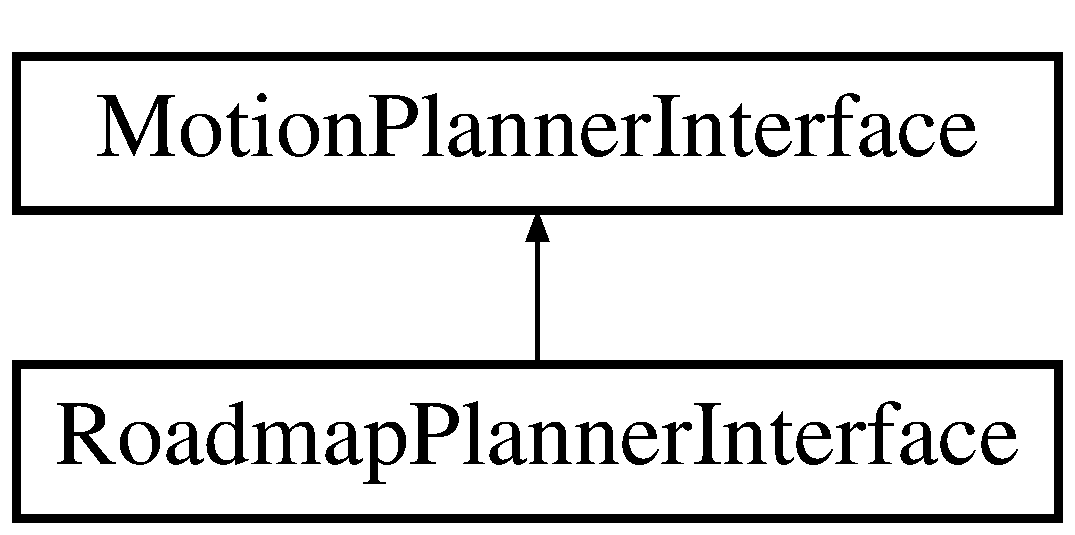
\includegraphics[height=2.000000cm]{classRoadmapPlannerInterface}
\end{center}
\end{figure}
\subsection*{Public Member Functions}
\begin{DoxyCompactItemize}
\item 
{\bfseries Roadmap\+Planner\+Interface} ({\bf C\+Space} $\ast$space)\label{classRoadmapPlannerInterface_a77adfc0acbb6b5babf35e3a6c18e04c1}

\item 
virtual bool {\bfseries Can\+Add\+Milestone} () const \label{classRoadmapPlannerInterface_a30063c13117e4435fcb364d46eac44bd}

\item 
virtual int {\bfseries Add\+Milestone} (const Config \&q)\label{classRoadmapPlannerInterface_ac75646b8f284e9e5a9f0ec82044e5574}

\item 
virtual void {\bfseries Get\+Milestone} (int i, Config \&q)\label{classRoadmapPlannerInterface_a2fb6766566cb1cdf58174e144890f98c}

\item 
virtual void {\bfseries Connect\+Hint} (int n)\label{classRoadmapPlannerInterface_a70724bfac7e68044dbff6c2d45351f66}

\item 
virtual bool {\bfseries Connect\+Hint} (int i, int j)\label{classRoadmapPlannerInterface_a9b6566d0d74d40e478ed954b96a157ed}

\item 
virtual int {\bfseries Plan\+More} ()\label{classRoadmapPlannerInterface_a8d4e2080b43a34f623e3108dc3e136d3}

\item 
virtual int {\bfseries Num\+Iterations} () const \label{classRoadmapPlannerInterface_a5dbe9b13ce491b487aa68098cbdd8d29}

\item 
virtual int {\bfseries Num\+Milestones} () const \label{classRoadmapPlannerInterface_ab5e87e08db4b8a574d099793fe8a8a59}

\item 
virtual int {\bfseries Num\+Components} () const \label{classRoadmapPlannerInterface_ad35643d1dcdec98d2eed2c5e2eceeeec}

\item 
virtual bool {\bfseries Is\+Connected} (int ma, int mb) const \label{classRoadmapPlannerInterface_a1c02edb8c839114114235c4d0a4abda5}

\item 
virtual void {\bfseries Get\+Path} (int ma, int mb, {\bf Milestone\+Path} \&path)\label{classRoadmapPlannerInterface_adf822a8f0427578c7df8ee0fd0eef5ac}

\item 
virtual void {\bfseries Get\+Roadmap} ({\bf Roadmap\+Planner} \&roadmap)\label{classRoadmapPlannerInterface_ae63cbe356b3fe7c76e0a7fb1987db6f8}

\end{DoxyCompactItemize}
\subsection*{Public Attributes}
\begin{DoxyCompactItemize}
\item 
{\bf Roadmap\+Planner} {\bfseries prm}\label{classRoadmapPlannerInterface_a2c290a15ea8d309c4f3ce5457e80f20b}

\item 
int {\bfseries knn}\label{classRoadmapPlannerInterface_a2de858ecc62bc3b357a220e5bcb80ea6}

\item 
double {\bfseries connection\+Threshold}\label{classRoadmapPlannerInterface_aeac732d09971dc2a4644549ccf028722}

\item 
int {\bfseries num\+Iters}\label{classRoadmapPlannerInterface_ac9eae34586605e405a71700f24e3de5d}

\end{DoxyCompactItemize}


The documentation for this class was generated from the following file\+:\begin{DoxyCompactItemize}
\item 
Any\+Motion\+Planner.\+cpp\end{DoxyCompactItemize}

\section{R\+R\+T\+Planner Class Reference}
\label{classRRTPlanner}\index{R\+R\+T\+Planner@{R\+R\+T\+Planner}}


A basic R\+RT (Rapidly-\/\+Exploring Random Tree) planner.  




{\ttfamily \#include $<$Motion\+Planner.\+h$>$}

Inheritance diagram for R\+R\+T\+Planner\+:\begin{figure}[H]
\begin{center}
\leavevmode
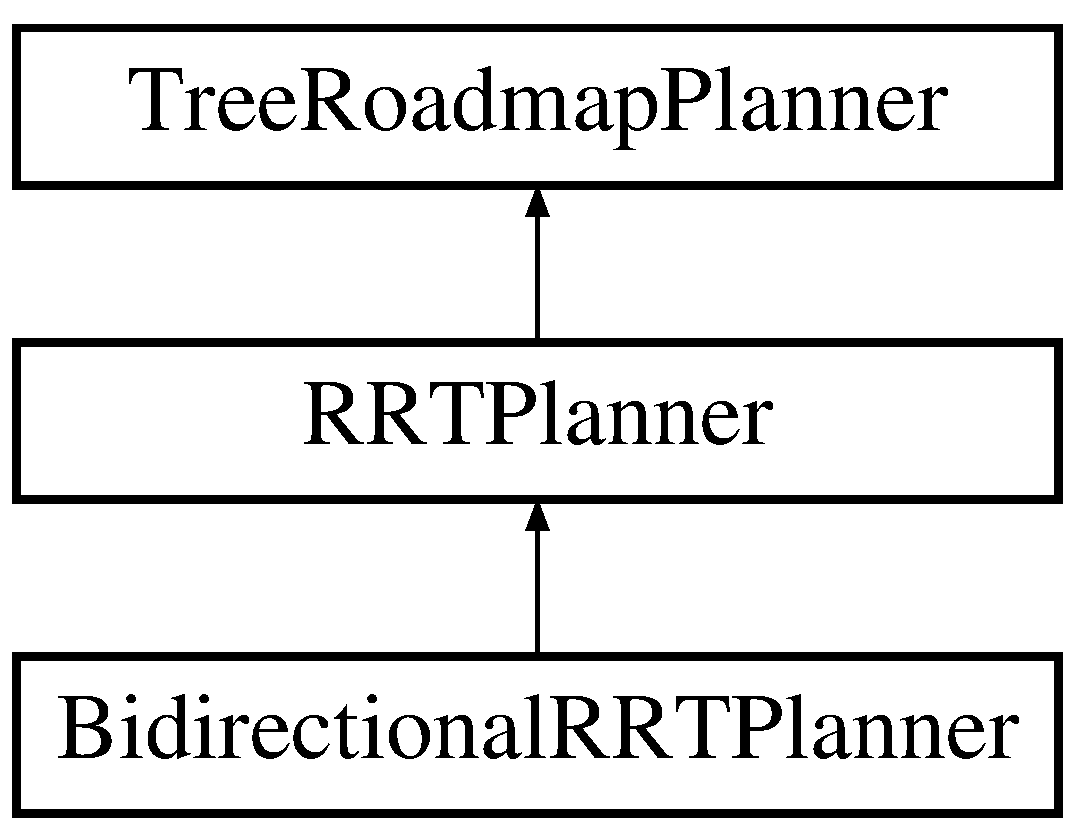
\includegraphics[height=3.000000cm]{classRRTPlanner}
\end{center}
\end{figure}
\subsection*{Public Member Functions}
\begin{DoxyCompactItemize}
\item 
{\bfseries R\+R\+T\+Planner} ({\bf C\+Space} $\ast$s)\label{classRRTPlanner_a7e05739b70e094e8c8db2d4e59d88c7c}

\item 
virtual Node $\ast$ {\bfseries Extend} ()\label{classRRTPlanner_a60465eda37372c30a88fffbb89d6ef77}

\end{DoxyCompactItemize}
\subsection*{Public Attributes}
\begin{DoxyCompactItemize}
\item 
double {\bfseries delta}\label{classRRTPlanner_a4d715600295aebd1f18d29c4e9dee1bd}

\end{DoxyCompactItemize}
\subsection*{Additional Inherited Members}


\subsection{Detailed Description}
A basic R\+RT (Rapidly-\/\+Exploring Random Tree) planner. 

Max distance to expand existing nodes is given in delta.

Currently this does not attempt to connect separate trees. 

The documentation for this class was generated from the following files\+:\begin{DoxyCompactItemize}
\item 
Motion\+Planner.\+h\item 
Motion\+Planner.\+cpp\end{DoxyCompactItemize}

\section{S\+B\+L\+Interface Class Reference}
\label{classSBLInterface}\index{S\+B\+L\+Interface@{S\+B\+L\+Interface}}
Inheritance diagram for S\+B\+L\+Interface\+:\begin{figure}[H]
\begin{center}
\leavevmode
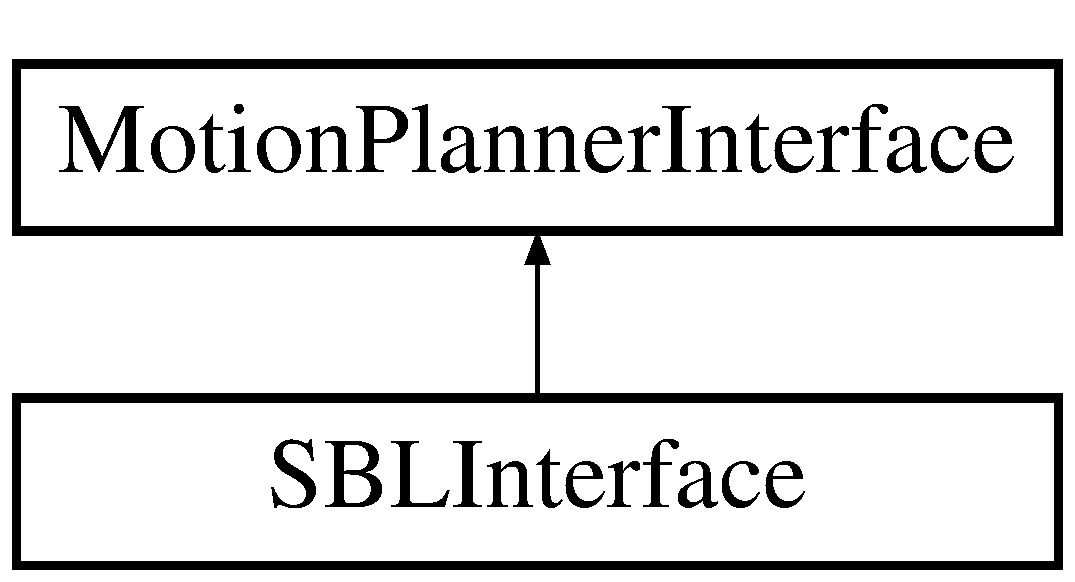
\includegraphics[height=2.000000cm]{classSBLInterface}
\end{center}
\end{figure}
\subsection*{Public Member Functions}
\begin{DoxyCompactItemize}
\item 
{\bfseries S\+B\+L\+Interface} ({\bf C\+Space} $\ast$space)\label{classSBLInterface_af696f2eb075ad3ac99477d4caa5b7ea3}

\item 
{\bfseries S\+B\+L\+Interface} ({\bf C\+Space} $\ast$space, bool grid, double grid\+Divs, int randomize\+Frequency)\label{classSBLInterface_afc33df95aaa9aa28c7795be70f4d460e}

\item 
void {\bfseries Init} (const Config \&q\+Start, const Config \&q\+Goal)\label{classSBLInterface_a41902b9740721fef100544f8bbf046b1}

\item 
virtual bool {\bfseries Can\+Add\+Milestone} () const \label{classSBLInterface_a0a41d52400a9bbb441f75c7f9798e561}

\item 
virtual int {\bfseries Add\+Milestone} (const Config \&q)\label{classSBLInterface_a5b0968f86076c51885d0e778047a49b2}

\item 
virtual void {\bfseries Get\+Milestone} (int i, Config \&q)\label{classSBLInterface_a8c8cc665a71b443806639a5259e549a6}

\item 
virtual int {\bfseries Plan\+More} ()\label{classSBLInterface_a676a4fc409b7387c76e30c0cd465ccda}

\item 
virtual int {\bfseries Num\+Iterations} () const \label{classSBLInterface_af41870c581eafdfbc48fd8f2e7601e59}

\item 
virtual int {\bfseries Num\+Milestones} () const \label{classSBLInterface_a0f23b1b83a783410af5112f4e5a57423}

\item 
virtual int {\bfseries Num\+Components} () const \label{classSBLInterface_adf31abc8d6efd1e130412d0d31f14bbb}

\item 
virtual bool {\bfseries Is\+Connected} (int ma, int mb) const \label{classSBLInterface_a8ddaea8dbe39145f7f77fc5799b4e996}

\item 
virtual void {\bfseries Get\+Path} (int ma, int mb, {\bf Milestone\+Path} \&path)\label{classSBLInterface_ab740abb21e614cc412b691c80a5b3eb0}

\item 
void {\bfseries Enumerate} (S\+B\+L\+Tree\+::\+Node $\ast$node, int index, {\bf Roadmap\+Planner} \&roadmap)\label{classSBLInterface_a3d4fa8f081896655c562793c78e347ac}

\item 
virtual void {\bfseries Get\+Roadmap} ({\bf Roadmap\+Planner} \&roadmap)\label{classSBLInterface_ac2d66ca5d75a7fa6a55db142360e564a}

\end{DoxyCompactItemize}
\subsection*{Public Attributes}
\begin{DoxyCompactItemize}
\item 
Smart\+Pointer$<$ {\bf S\+B\+L\+Planner} $>$ {\bfseries sbl}\label{classSBLInterface_a78bfe02e938e062c74c2c7b889495572}

\item 
Config {\bfseries q\+Start}\label{classSBLInterface_a4e1e581845aedcf21175c4b5c4d46645}

\item 
Config {\bfseries q\+Goal}\label{classSBLInterface_ae303831c29066d157859d56cdee6ea19}

\end{DoxyCompactItemize}


The documentation for this class was generated from the following file\+:\begin{DoxyCompactItemize}
\item 
Any\+Motion\+Planner.\+cpp\end{DoxyCompactItemize}

\section{S\+B\+L\+Planner Class Reference}
\label{classSBLPlanner}\index{S\+B\+L\+Planner@{S\+B\+L\+Planner}}


The S\+BL motion planner.  




{\ttfamily \#include $<$S\+B\+L.\+h$>$}

Inheritance diagram for S\+B\+L\+Planner\+:\begin{figure}[H]
\begin{center}
\leavevmode
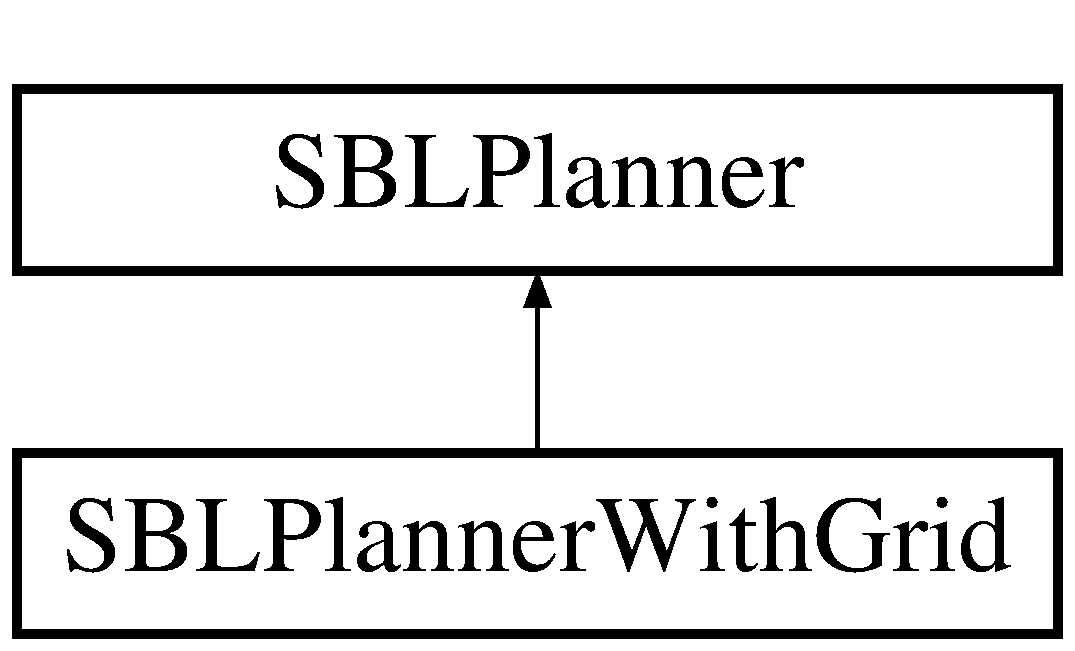
\includegraphics[height=2.000000cm]{classSBLPlanner}
\end{center}
\end{figure}
\subsection*{Public Types}
\begin{DoxyCompactItemize}
\item 
typedef S\+B\+L\+Tree\+::\+Node {\bfseries Node}\label{classSBLPlanner_a169f36f0433ca8891996f18efd99c2c5}

\item 
typedef {\bf S\+B\+L\+Tree\+::\+Edge\+Info} {\bfseries Edge\+Info}\label{classSBLPlanner_a017acd60bfdb134c65c3892a9b3de842}

\end{DoxyCompactItemize}
\subsection*{Public Member Functions}
\begin{DoxyCompactItemize}
\item 
{\bfseries S\+B\+L\+Planner} ({\bf C\+Space} $\ast$)\label{classSBLPlanner_aba6b0ad96b263b92f5614a50faf51657}

\item 
virtual void {\bfseries Cleanup} ()\label{classSBLPlanner_a9c9151f0f8d42922446ce9f3e262a8bd}

\item 
virtual void {\bfseries Init} (const Config \&q\+Start, const Config \&q\+Goal)\label{classSBLPlanner_a6792ee71a70539e7ed11724e3d04343b}

\item 
virtual bool {\bfseries Extend} ()\label{classSBLPlanner_a3452dcaba7bd47077db65b34b44a7896}

\item 
virtual Node $\ast$ {\bfseries Pick\+Connection} ({\bf S\+B\+L\+Tree} $\ast$t, const Config \&x)\label{classSBLPlanner_ac025a72b7e61fc770bd68d5e5e9abc3d}

\item 
bool {\bfseries Is\+Done} () const \label{classSBLPlanner_a4fb16b752eb517eedea2d1f07c78f4de}

\item 
void {\bfseries Create\+Path} ({\bf Milestone\+Path} \&path) const \label{classSBLPlanner_ae7db86e45375469860f9e25c4bb1a1ee}

\item 
bool {\bfseries Check\+Path} (Node $\ast$n\+Start, Node $\ast$n\+Goal)\label{classSBLPlanner_aecba9031d2cdc33bd4377fce2c80bf96}

\end{DoxyCompactItemize}
\subsection*{Public Attributes}
\begin{DoxyCompactItemize}
\item 
{\bf C\+Space} $\ast$ {\bfseries space}\label{classSBLPlanner_ae967b2aec44781dfc10390fc4271c4c9}

\item 
double {\bfseries max\+Extend\+Distance}\label{classSBLPlanner_a5f708507dc2086c6021fc71b521b89be}

\item 
int {\bfseries max\+Extend\+Iters}\label{classSBLPlanner_a654954ceca455738212fec15ec5b65c2}

\item 
double {\bfseries edge\+Connection\+Threshold}\label{classSBLPlanner_ae89e7029457ab560ef036aa6815b6420}

\item 
int {\bfseries num\+Iters}\label{classSBLPlanner_a04d8e3976fd27a1e13afacedcf54c57e}

\item 
{\bf S\+B\+L\+Tree} $\ast$ {\bfseries t\+Start}\label{classSBLPlanner_a62122ad392d5c41577b7007f43e352aa}

\item 
{\bf S\+B\+L\+Tree} $\ast$ {\bfseries t\+Goal}\label{classSBLPlanner_a868c99b7fdb9304260634336b56e70e4}

\item 
std\+::list$<$ {\bf Edge\+Info} $>$ {\bfseries output\+Path}\label{classSBLPlanner_aee8ab7d492e1e868b918714a233d931a}

\end{DoxyCompactItemize}


\subsection{Detailed Description}
The S\+BL motion planner. 

Call Init() with the start and goal configuration. While Is\+Done() returns false, call Extend() . Retrieve the path with Create\+Path().

Parameters are max\+Extend\+Distance, max\+Extend\+Iters, edge\+Connection\+Threshold. max\+Extend\+Distance is the radius of the neighborhood sampling. max\+Extend\+Iters is the number of iters of shrinking the neighborhood sampling radius until we quit. edge\+Connection\+Threshold is the minimum distance required for a connection between the two trees. 

The documentation for this class was generated from the following files\+:\begin{DoxyCompactItemize}
\item 
S\+B\+L.\+h\item 
S\+B\+L.\+cpp\end{DoxyCompactItemize}

\section{S\+B\+L\+Planner\+With\+Grid Class Reference}
\label{classSBLPlannerWithGrid}\index{S\+B\+L\+Planner\+With\+Grid@{S\+B\+L\+Planner\+With\+Grid}}


An S\+BL planner whose trees use grids for point location.  




{\ttfamily \#include $<$S\+B\+L.\+h$>$}

Inheritance diagram for S\+B\+L\+Planner\+With\+Grid\+:\begin{figure}[H]
\begin{center}
\leavevmode
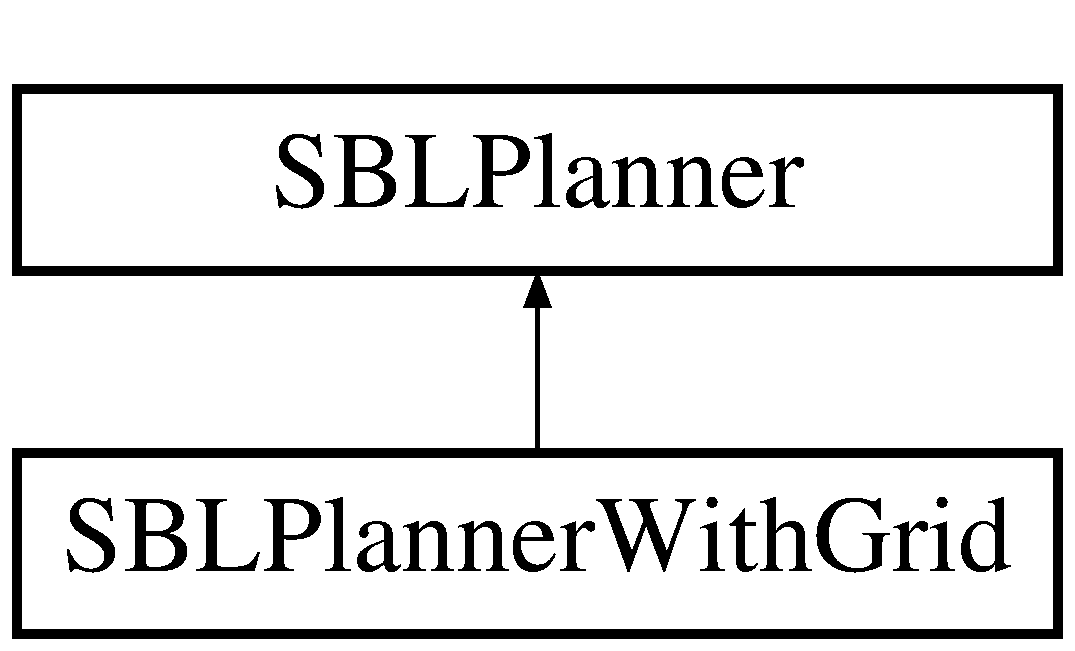
\includegraphics[height=2.000000cm]{classSBLPlannerWithGrid}
\end{center}
\end{figure}
\subsection*{Public Member Functions}
\begin{DoxyCompactItemize}
\item 
{\bfseries S\+B\+L\+Planner\+With\+Grid} ({\bf C\+Space} $\ast$)\label{classSBLPlannerWithGrid_ab190515375538d65152fb87a377957e8}

\item 
virtual void {\bfseries Cleanup} ()\label{classSBLPlannerWithGrid_aae4120821b162b089edb3f3e192b3805}

\item 
virtual void {\bfseries Init} (const Config \&q\+Start, const Config \&q\+Goal)\label{classSBLPlannerWithGrid_a877d3616dbe353e4005d712fe203368c}

\item 
virtual bool {\bfseries Extend} ()\label{classSBLPlannerWithGrid_a15fceeb69521215cfb55d7a90f4098a3}

\item 
virtual Node $\ast$ {\bfseries Pick\+Connection} ({\bf S\+B\+L\+Tree} $\ast$t, const Config \&x)\label{classSBLPlannerWithGrid_a1a6adeae4cf85b853a525c8bb9d5b0b2}

\item 
void {\bfseries Randomize\+Subset} ()\label{classSBLPlannerWithGrid_a7d702a676538d8c9ed892dcb4380d8c9}

\end{DoxyCompactItemize}
\subsection*{Public Attributes}
\begin{DoxyCompactItemize}
\item 
int {\bfseries num\+Iters\+Per\+Randomize}\label{classSBLPlannerWithGrid_a224e9dc7e6f695172ea59dc4a3a040c0}

\item 
double {\bfseries grid\+Division}\label{classSBLPlannerWithGrid_a87e6c4778cde4b92f658bf4b091658d0}

\end{DoxyCompactItemize}
\subsection*{Additional Inherited Members}


\subsection{Detailed Description}
An S\+BL planner whose trees use grids for point location. 

Every num\+Iters\+Per\+Randomize Extend() iterations, the grid dimensions are randomized. They use a 3-\/d grid with division grid\+Division. 

The documentation for this class was generated from the following files\+:\begin{DoxyCompactItemize}
\item 
S\+B\+L.\+h\item 
S\+B\+L.\+cpp\end{DoxyCompactItemize}

\section{S\+B\+L\+P\+RT Class Reference}
\label{classSBLPRT}\index{S\+B\+L\+P\+RT@{S\+B\+L\+P\+RT}}


A probabilistic roadmap of trees, where S\+BL is used for local planning.  




{\ttfamily \#include $<$S\+B\+L.\+h$>$}

\subsection*{Public Types}
\begin{DoxyCompactItemize}
\item 
typedef S\+B\+L\+Tree\+::\+Node {\bfseries Node}\label{classSBLPRT_a8c9c3931b90604b1ef785369a2ca0560}

\item 
typedef {\bf S\+B\+L\+Tree\+::\+Edge\+Info} {\bfseries Edge\+Info}\label{classSBLPRT_a963e472e4836d7f38bfe4e4234e68310}

\item 
typedef Graph\+::\+Undirected\+Graph$<$ {\bf S\+B\+L\+Tree} $\ast$, {\bf Milestone\+Path} $>$ {\bfseries Roadmap}\label{classSBLPRT_ae1fb7f3c065af93b4f1b1d4e8ef0876a}

\end{DoxyCompactItemize}
\subsection*{Public Member Functions}
\begin{DoxyCompactItemize}
\item 
{\bfseries S\+B\+L\+P\+RT} ({\bf C\+Space} $\ast$s)\label{classSBLPRT_ae9452ac5e184677d048cee75bb290c79}

\item 
virtual void {\bfseries Cleanup} ()\label{classSBLPRT_a7bd6839a7f47b2b13c09a0de6a8c4f73}

\item 
int {\bfseries Add\+Seed} (const Config \&q)\label{classSBLPRT_a2ff67972faaf1e02b84a7838ed8fef34}

\item 
pair$<$ int, int $>$ {\bfseries Expand} ()\label{classSBLPRT_a92cc85ba0385617c7157ff30221d9a5c}

\item 
int {\bfseries Expand\+Tree} (int t)\label{classSBLPRT_a57fb164bb322f0fe9459d0f56e00c328}

\item 
void {\bfseries Add\+Roadmap\+Edges\+If\+Below\+Threshold} (double distance\+Threshold)\label{classSBLPRT_adf926ead4cb1e8a2b0c8fe953aae475f}

\item 
void {\bfseries Add\+Roadmap\+Edge} (int i, int j)\label{classSBLPRT_a380279cce525c5892b39a43c0f27b3f6}

\item 
bool {\bfseries Is\+Edge\+Connected} (int i, int j) const \label{classSBLPRT_a28e8316b833653e0eedeee3fee914d88}

\item 
bool {\bfseries Is\+Seed\+Fully\+Connected} (int i) const \label{classSBLPRT_a7490ea756ebbd3fe8d8e6d4a62eefda5}

\item 
bool {\bfseries Are\+Seeds\+Connected} (int i, int j) const \label{classSBLPRT_a1f3442d07ea2f9d1636aa7d03f074c67}

\item 
void {\bfseries Create\+Path} (int i, int j, {\bf Milestone\+Path} \&path)\label{classSBLPRT_afd15fb5bcf265fe81c8e9c69fd3d1de6}

\item 
virtual pair$<$ int, Node $\ast$ $>$ {\bfseries Pick\+Connection} (int t, Node $\ast$n)\label{classSBLPRT_a893cb4b0edad55c26b2c39f6469c37e2}

\item 
int {\bfseries Pick\+Random\+Adjacent\+Tree} (int t)\label{classSBLPRT_aaf3da20a02334ca511b15266baabab15}

\item 
int {\bfseries Pick\+Closest\+Adjacent\+Tree} (int t, const Config \&x)\label{classSBLPRT_afcf10b24a3cbd317e91628e808244dcb}

\item 
Node $\ast$ {\bfseries Get\+Closest\+Node} (int t, const Config \&x)\label{classSBLPRT_aa37e6a476c614d0e1abb2b46b18d8179}

\item 
Node $\ast$ {\bfseries Pick\+Node} (int t)\label{classSBLPRT_a94bf663371d2d9a3a2c79d522cf661d7}

\end{DoxyCompactItemize}
\subsection*{Public Attributes}
\begin{DoxyCompactItemize}
\item 
{\bf C\+Space} $\ast$ {\bfseries space}\label{classSBLPRT_a3a44566bfa70d68401d977805a3616bf}

\item 
double {\bfseries max\+Extend\+Distance}\label{classSBLPRT_a29b6b5107aa07ef314157a309621ed00}

\item 
int {\bfseries max\+Extend\+Iters}\label{classSBLPRT_a77dfdd94494e772c22ec865f16f8d06a}

\item 
double {\bfseries default\+P\+Pick\+Closest\+Tree}\label{classSBLPRT_a4cc930706229025c08249e1db9eb2b65}

\item 
double {\bfseries default\+P\+Pick\+Closest\+Node}\label{classSBLPRT_aa53e115e8f35da2cc241bef584a5c17f}

\item 
int {\bfseries num\+Iters}\label{classSBLPRT_ae81b491304d06e4bd47faab688e0bedb}

\item 
Roadmap {\bfseries roadmap}\label{classSBLPRT_ab868467342df45aba0efbde15464294f}

\item 
Graph\+::\+Connected\+Components {\bfseries ccs}\label{classSBLPRT_ad6ea8152160bd6227541b68cde7dfe63}

\end{DoxyCompactItemize}


\subsection{Detailed Description}
A probabilistic roadmap of trees, where S\+BL is used for local planning. 

Permitted connections are represented by edges in an undirected graph. Plans are attempted only along these edges. An edge has a corresponding \doxyref{Milestone\+Path}{p.}{classMilestonePath} which will contain the path between the seeds once planning is complete. 

The documentation for this class was generated from the following files\+:\begin{DoxyCompactItemize}
\item 
S\+B\+L.\+h\item 
S\+B\+L.\+cpp\end{DoxyCompactItemize}

\section{S\+B\+L\+P\+R\+T\+Interface Class Reference}
\label{classSBLPRTInterface}\index{S\+B\+L\+P\+R\+T\+Interface@{S\+B\+L\+P\+R\+T\+Interface}}
Inheritance diagram for S\+B\+L\+P\+R\+T\+Interface\+:\begin{figure}[H]
\begin{center}
\leavevmode
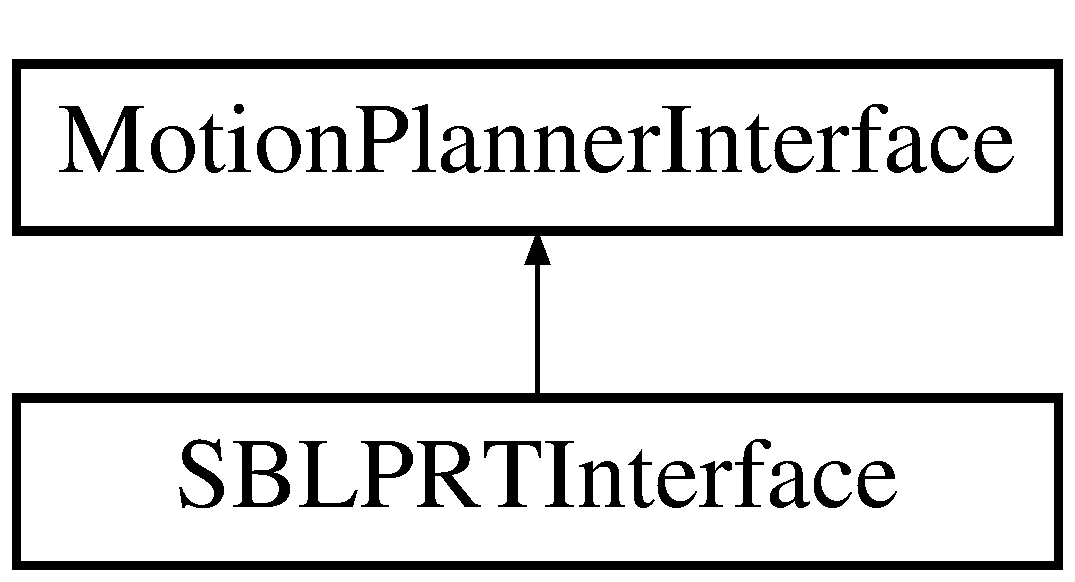
\includegraphics[height=2.000000cm]{classSBLPRTInterface}
\end{center}
\end{figure}
\subsection*{Public Member Functions}
\begin{DoxyCompactItemize}
\item 
{\bfseries S\+B\+L\+P\+R\+T\+Interface} ({\bf C\+Space} $\ast$space)\label{classSBLPRTInterface_a58e87356bb6eae4e870e0a70e6e38bf7}

\item 
virtual bool {\bfseries Can\+Add\+Milestone} () const \label{classSBLPRTInterface_a58763e501106088127d09ea32844e2c7}

\item 
virtual int {\bfseries Add\+Milestone} (const Config \&q)\label{classSBLPRTInterface_adbddb57c56bb128aaf779e38aa14b975}

\item 
virtual void {\bfseries Get\+Milestone} (int i, Config \&q)\label{classSBLPRTInterface_a13d5d64522fb9e8a408179d29ea77727}

\item 
virtual void {\bfseries Connect\+Hint} (int i)\label{classSBLPRTInterface_aeebdd35d4728d71aecb150e1c1200607}

\item 
virtual bool {\bfseries Connect\+Hint} (int i, int j)\label{classSBLPRTInterface_af9e1e16778d6b93306992405905f7b64}

\item 
virtual int {\bfseries Plan\+More} ()\label{classSBLPRTInterface_a6231771187d70ef22005161b51ee6a14}

\item 
virtual int {\bfseries Num\+Iterations} () const \label{classSBLPRTInterface_a00019abb6796be7544d41a73779a443b}

\item 
virtual int {\bfseries Num\+Milestones} () const \label{classSBLPRTInterface_a2e828ce36fc8c49706b302a27088cd7d}

\item 
virtual int {\bfseries Num\+Components} () const \label{classSBLPRTInterface_adbaef4e9d7cf2de4d278bd82240d2697}

\item 
virtual bool {\bfseries Is\+Connected} (int ma, int mb) const \label{classSBLPRTInterface_aeab450362f1cfa93d6abcaf7f7c676df}

\item 
virtual void {\bfseries Get\+Path} (int ma, int mb, {\bf Milestone\+Path} \&path)\label{classSBLPRTInterface_a7fd6e33cd618ccddabfadba769e5f565}

\end{DoxyCompactItemize}
\subsection*{Public Attributes}
\begin{DoxyCompactItemize}
\item 
{\bf S\+B\+L\+P\+RT} {\bfseries sblprt}\label{classSBLPRTInterface_a736a22815895b17a90e2d1adf1fa0b0a}

\end{DoxyCompactItemize}


The documentation for this class was generated from the following file\+:\begin{DoxyCompactItemize}
\item 
Any\+Motion\+Planner.\+cpp\end{DoxyCompactItemize}

\section{S\+B\+L\+Subdivision Class Reference}
\label{classSBLSubdivision}\index{S\+B\+L\+Subdivision@{S\+B\+L\+Subdivision}}


A grid-\/based subdivision to be used for S\+BL.  




{\ttfamily \#include $<$S\+B\+L\+Tree.\+h$>$}

\subsection*{Public Types}
\begin{DoxyCompactItemize}
\item 
typedef S\+B\+L\+Tree\+::\+Node {\bfseries Node}\label{classSBLSubdivision_a7324b5c74750880cec033afb37038a2c}

\end{DoxyCompactItemize}
\subsection*{Public Member Functions}
\begin{DoxyCompactItemize}
\item 
{\bfseries S\+B\+L\+Subdivision} (int mapped\+Dims)\label{classSBLSubdivision_afa9f36ebe972bfaaaca77d1227c01c60}

\item 
void {\bfseries Clear} ()\label{classSBLSubdivision_a72951c73404d234b283b3dc9e3edb3fa}

\item 
void {\bfseries Randomize\+Subset} ()\label{classSBLSubdivision_aff7fca9f5d9636197218d868c3437b83}

\item 
void {\bfseries Add\+Point} (Node $\ast$)\label{classSBLSubdivision_af03a3de4a38b9f8265b0ecce9a3baffa}

\item 
void {\bfseries Remove\+Point} (Node $\ast$)\label{classSBLSubdivision_a04517be59b8fae13417516e44c247db8}

\item 
Node $\ast$ {\bfseries Pick\+Point} (const Config \&x)\label{classSBLSubdivision_a2803f47f6dd4191dba26b7852e4d9ba3}

\item 
Node $\ast$ {\bfseries Pick\+Random} ()\label{classSBLSubdivision_a503125a633d392f8785983750e229a80}

\end{DoxyCompactItemize}
\subsection*{Public Attributes}
\begin{DoxyCompactItemize}
\item 
Vector {\bfseries h}\label{classSBLSubdivision_ad4726b6334a853199e72461c8428fabc}

\item 
std\+::vector$<$ int $>$ {\bfseries subset}\label{classSBLSubdivision_ac6a572c6a25fc396240e63f4b41ee610}

\item 
Geometry\+::\+Grid\+Subdivision {\bfseries subdiv}\label{classSBLSubdivision_a0f7871c89cf476680167e93a19d92f65}

\item 
Vector {\bfseries temp}\label{classSBLSubdivision_a3a39403d855f390b6120a27028c46fbe}

\end{DoxyCompactItemize}


\subsection{Detailed Description}
A grid-\/based subdivision to be used for S\+BL. 

The grid operates on certain dimensions of the configuration. Specifically, it picks mapped\+Dims dimensions at random from the full configuration space, and divides the space in those dimensions into cells of width h. If the mapped dimension is that of index k.

N\+O\+TE\+: h must be initialized to the \# of dims in the configuration space, and containing some cell width value, say 0.\+1. \begin{DoxyRefDesc}{Todo}
\item[{\bf Todo}]Do a defualt initialization of h. \end{DoxyRefDesc}


The documentation for this class was generated from the following files\+:\begin{DoxyCompactItemize}
\item 
S\+B\+L\+Tree.\+h\item 
S\+B\+L\+Tree.\+cpp\end{DoxyCompactItemize}

\section{S\+B\+L\+Tree Class Reference}
\label{classSBLTree}\index{S\+B\+L\+Tree@{S\+B\+L\+Tree}}


A tree of configurations to be used in the S\+BL motion planner.  




{\ttfamily \#include $<$S\+B\+L\+Tree.\+h$>$}

Inheritance diagram for S\+B\+L\+Tree\+:\begin{figure}[H]
\begin{center}
\leavevmode
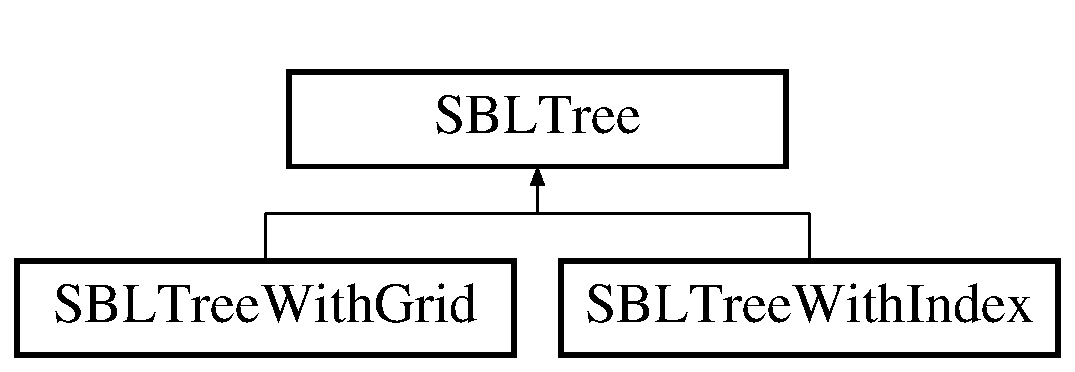
\includegraphics[height=2.000000cm]{classSBLTree}
\end{center}
\end{figure}
\subsection*{Classes}
\begin{DoxyCompactItemize}
\item 
struct {\bf Edge\+Info}
\end{DoxyCompactItemize}
\subsection*{Public Types}
\begin{DoxyCompactItemize}
\item 
typedef Graph\+::\+Tree\+Node$<$ Config, Smart\+Pointer$<$ {\bf Edge\+Planner} $>$ $>$ {\bfseries Node}\label{classSBLTree_a91f69b90c6e2fc372a31c97a87d3aa15}

\end{DoxyCompactItemize}
\subsection*{Public Member Functions}
\begin{DoxyCompactItemize}
\item 
{\bfseries S\+B\+L\+Tree} ({\bf C\+Space} $\ast$)\label{classSBLTree_a367a93a43d7cb01c34136b77b555ca49}

\item 
virtual void {\bfseries Cleanup} ()\label{classSBLTree_ac075223ea0a5f0a01c9df668ead2ecae}

\item 
virtual void {\bfseries Init} (const Config \&q\+Start)\label{classSBLTree_ae14637d72a51bb5fe7e4c98b819cbf90}

\item 
virtual Node $\ast$ {\bfseries Extend} (double max\+Distance, int max\+Iters)\label{classSBLTree_a015ba93ecff317cb1d72eb596e63fe1e}

\item 
virtual void {\bfseries Add\+Milestone} (Node $\ast$n)\label{classSBLTree_a31c4852082df50820fe30c590173b96c}

\item 
virtual void {\bfseries Remove\+Milestone} (Node $\ast$n)\label{classSBLTree_ab58366d9da8aa521389fc2db6a4175ac}

\item 
virtual Node $\ast$ {\bfseries Pick\+Expand} ()\label{classSBLTree_a87a32676fd734538b699b13c9c37b4cf}

\item 
Node $\ast$ {\bfseries Add\+Milestone} (const Config \&q)\label{classSBLTree_a1061a3c9ead4d26572d858c40b3f0ed9}

\item 
bool {\bfseries Has\+Node} (Node $\ast$n) const \label{classSBLTree_aa00f8a31a0590bdb7885693d1f4e7f2b}

\item 
Node $\ast$ {\bfseries Add\+Child} (Node $\ast$n, const Config \&x)\label{classSBLTree_a1699cb550b424bc24e50d6b478fbeca0}

\item 
Node $\ast$ {\bfseries Find\+Closest} (const Config \&x)\label{classSBLTree_a6346a7340ab1316894ef0de334cf2581}

\end{DoxyCompactItemize}
\subsection*{Static Public Member Functions}
\begin{DoxyCompactItemize}
\item 
static bool {\bfseries Check\+Path} ({\bf S\+B\+L\+Tree} $\ast$ts, Node $\ast$ns, {\bf S\+B\+L\+Tree} $\ast$tg, Node $\ast$ng, std\+::list$<$ {\bf Edge\+Info} $>$ \&output\+Path)\label{classSBLTree_ad12520b6429ecf48a836123af2d4f59e}

\end{DoxyCompactItemize}
\subsection*{Public Attributes}
\begin{DoxyCompactItemize}
\item 
{\bf C\+Space} $\ast$ {\bfseries space}\label{classSBLTree_abca592f0e583e6ddc032c8dc65ba0663}

\item 
Node $\ast$ {\bfseries root}\label{classSBLTree_a5a3bfe68e29b679b01266c523f1fcded}

\end{DoxyCompactItemize}


\subsection{Detailed Description}
A tree of configurations to be used in the S\+BL motion planner. 

The documentation for this class was generated from the following files\+:\begin{DoxyCompactItemize}
\item 
S\+B\+L\+Tree.\+h\item 
S\+B\+L\+Tree.\+cpp\end{DoxyCompactItemize}

\section{S\+B\+L\+Tree\+With\+Grid Class Reference}
\label{classSBLTreeWithGrid}\index{S\+B\+L\+Tree\+With\+Grid@{S\+B\+L\+Tree\+With\+Grid}}


An S\+BL motion planner that uses a \doxyref{S\+B\+L\+Subdivision}{p.}{classSBLSubdivision} to pick the next node to expand, and nodes to connect.  




{\ttfamily \#include $<$S\+B\+L\+Tree.\+h$>$}

Inheritance diagram for S\+B\+L\+Tree\+With\+Grid\+:\begin{figure}[H]
\begin{center}
\leavevmode
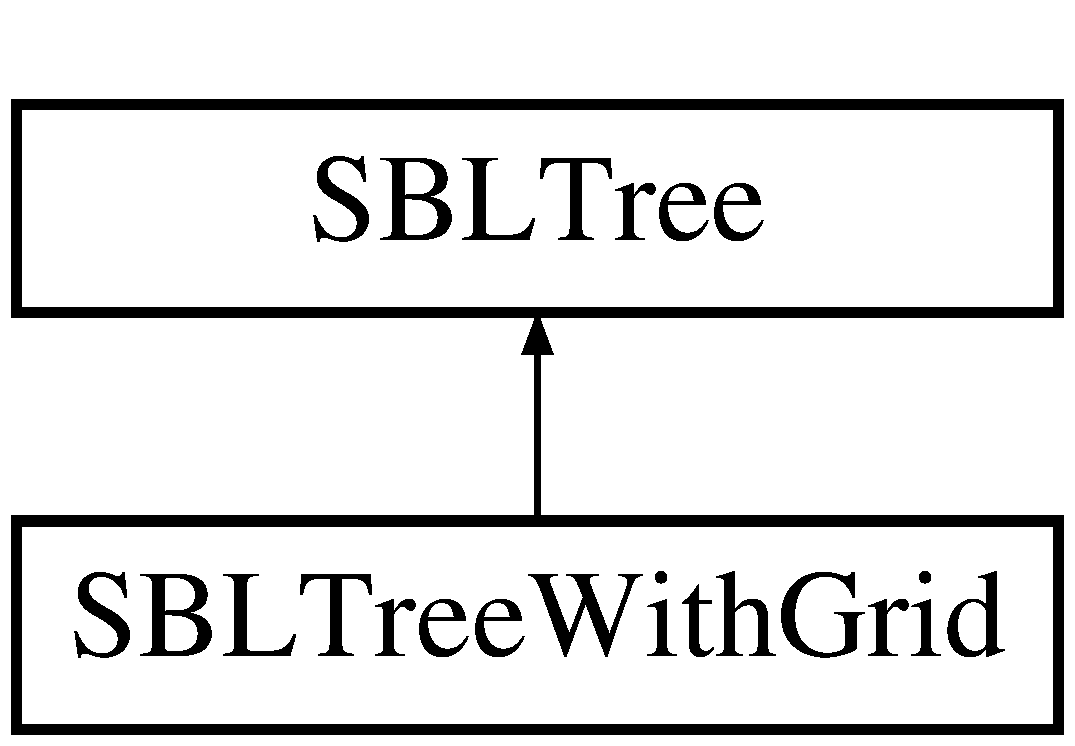
\includegraphics[height=2.000000cm]{classSBLTreeWithGrid}
\end{center}
\end{figure}
\subsection*{Public Member Functions}
\begin{DoxyCompactItemize}
\item 
{\bfseries S\+B\+L\+Tree\+With\+Grid} ({\bf C\+Space} $\ast$)\label{classSBLTreeWithGrid_ac106c04d4f71656f7acc37a8e14cee5c}

\item 
virtual void {\bfseries Init} (const Config \&q\+Start)\label{classSBLTreeWithGrid_ace63cb47c374eefcf72bd45d0473588f}

\item 
virtual void {\bfseries Cleanup} ()\label{classSBLTreeWithGrid_a651e8f6b2a93f0da4ad80f21e3ab5127}

\item 
void {\bf Init\+Default\+Grid} (int num\+Dims, double h)
\item 
void {\bf Randomize\+Subset} ()\label{classSBLTreeWithGrid_a92883bf5d7b2644b11ce4284c6686613}

\begin{DoxyCompactList}\small\item\em Randomizes the dimensions of the grid divisions Astart,Agoal. \end{DoxyCompactList}\item 
virtual void {\bfseries Add\+Milestone} (Node $\ast$n)\label{classSBLTreeWithGrid_a84d78bd772bff47ab62c2ab6116fed29}

\item 
virtual void {\bfseries Remove\+Milestone} (Node $\ast$n)\label{classSBLTreeWithGrid_a6268cb8a715fc91213bef8cd37583aec}

\item 
virtual Node $\ast$ {\bfseries Pick\+Expand} ()\label{classSBLTreeWithGrid_a41436200ed3b8ed356253eaafb93d2e2}

\item 
Node $\ast$ {\bfseries Find\+Nearby} (const Config \&x)\label{classSBLTreeWithGrid_a497fc9e0f9aaedce8b39ccd76ade2169}

\end{DoxyCompactItemize}
\subsection*{Public Attributes}
\begin{DoxyCompactItemize}
\item 
{\bf S\+B\+L\+Subdivision} {\bfseries A}\label{classSBLTreeWithGrid_ac20b45e8b9a9c21750e596346ca6aeef}

\end{DoxyCompactItemize}
\subsection*{Additional Inherited Members}


\subsection{Detailed Description}
An S\+BL motion planner that uses a \doxyref{S\+B\+L\+Subdivision}{p.}{classSBLSubdivision} to pick the next node to expand, and nodes to connect. 

\subsection{Member Function Documentation}
\index{S\+B\+L\+Tree\+With\+Grid@{S\+B\+L\+Tree\+With\+Grid}!Init\+Default\+Grid@{Init\+Default\+Grid}}
\index{Init\+Default\+Grid@{Init\+Default\+Grid}!S\+B\+L\+Tree\+With\+Grid@{S\+B\+L\+Tree\+With\+Grid}}
\subsubsection[{Init\+Default\+Grid(int num\+Dims, double h)}]{\setlength{\rightskip}{0pt plus 5cm}void S\+B\+L\+Tree\+With\+Grid\+::\+Init\+Default\+Grid (
\begin{DoxyParamCaption}
\item[{int}]{num\+Dims, }
\item[{double}]{h}
\end{DoxyParamCaption}
)}\label{classSBLTreeWithGrid_a650330cfd33c0e2010a894321c918ee1}
Initializes the grids Astart,Agoal to a configuration space of num\+Dims dimensions, uniform cell width of h 

The documentation for this class was generated from the following files\+:\begin{DoxyCompactItemize}
\item 
S\+B\+L\+Tree.\+h\item 
S\+B\+L\+Tree.\+cpp\end{DoxyCompactItemize}

\section{S\+B\+L\+Tree\+With\+Index Class Reference}
\label{classSBLTreeWithIndex}\index{S\+B\+L\+Tree\+With\+Index@{S\+B\+L\+Tree\+With\+Index}}


An \doxyref{S\+B\+L\+Tree}{p.}{classSBLTree} with a node index.  




{\ttfamily \#include $<$S\+B\+L\+Tree.\+h$>$}

Inheritance diagram for S\+B\+L\+Tree\+With\+Index\+:\begin{figure}[H]
\begin{center}
\leavevmode
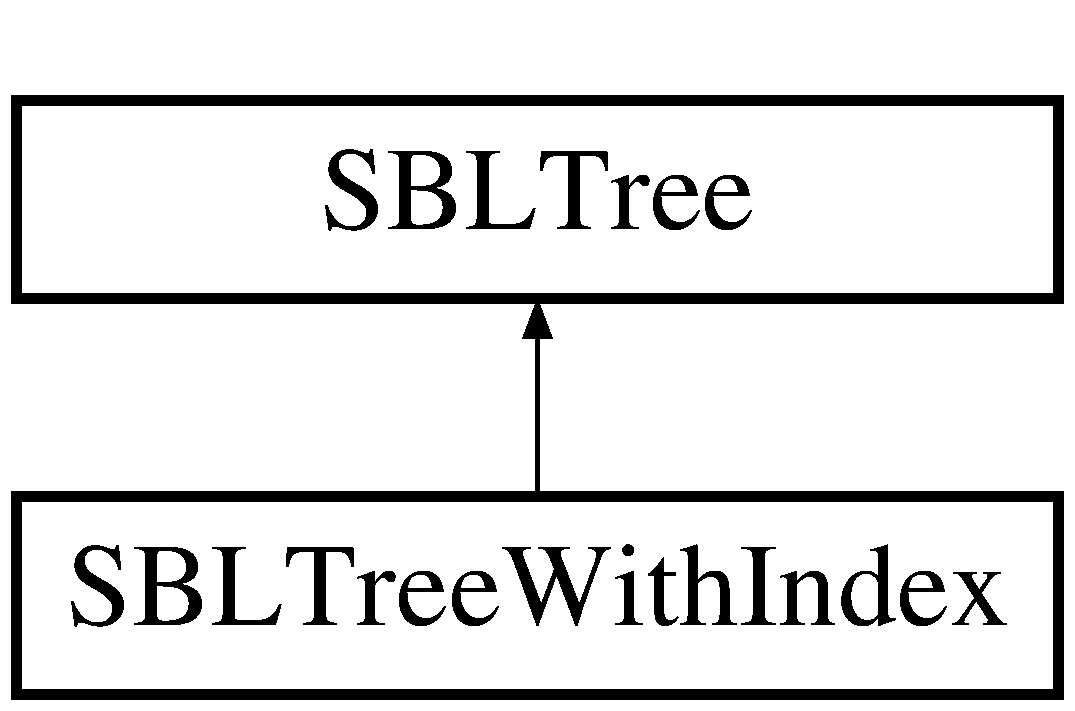
\includegraphics[height=2.000000cm]{classSBLTreeWithIndex}
\end{center}
\end{figure}
\subsection*{Public Member Functions}
\begin{DoxyCompactItemize}
\item 
{\bfseries S\+B\+L\+Tree\+With\+Index} ({\bf C\+Space} $\ast$)\label{classSBLTreeWithIndex_a07257d87351cf8e96dd308d4c5082601}

\item 
virtual void {\bfseries Cleanup} ()\label{classSBLTreeWithIndex_a725aa5267317ddfc9352c6fee40161a2}

\item 
virtual void {\bfseries Add\+Milestone} (Node $\ast$n)\label{classSBLTreeWithIndex_aade92f9349e2fb3155c80b35c3a00802}

\item 
virtual void {\bfseries Remove\+Milestone} (Node $\ast$n)\label{classSBLTreeWithIndex_a71861f0c670993112cfab0486c48cabb}

\item 
virtual Node $\ast$ {\bfseries Pick\+Expand} ()\label{classSBLTreeWithIndex_acb5aaf447ac0335f6406bb6dc6d7b76a}

\item 
Node $\ast$ {\bfseries Pick\+Random} () const \label{classSBLTreeWithIndex_ab02f40c75ba2f1cf04d9dbc809dd09fb}

\end{DoxyCompactItemize}
\subsection*{Public Attributes}
\begin{DoxyCompactItemize}
\item 
std\+::vector$<$ Node $\ast$ $>$ {\bfseries index}\label{classSBLTreeWithIndex_a8be39ea55edeab4600e75a7596de2ac7}

\end{DoxyCompactItemize}
\subsection*{Additional Inherited Members}


\subsection{Detailed Description}
An \doxyref{S\+B\+L\+Tree}{p.}{classSBLTree} with a node index. 

The documentation for this class was generated from the following files\+:\begin{DoxyCompactItemize}
\item 
S\+B\+L\+Tree.\+h\item 
S\+B\+L\+Tree.\+cpp\end{DoxyCompactItemize}

\section{Bisection\+Epsilon\+Edge\+Planner\+:\+:Segment Struct Reference}
\label{structBisectionEpsilonEdgePlanner_1_1Segment}\index{Bisection\+Epsilon\+Edge\+Planner\+::\+Segment@{Bisection\+Epsilon\+Edge\+Planner\+::\+Segment}}
\subsection*{Public Member Functions}
\begin{DoxyCompactItemize}
\item 
bool {\bfseries operator$<$} (const {\bf Segment} \&s) const \label{structBisectionEpsilonEdgePlanner_1_1Segment_a7a21c6b86f6f02ce54e2ae81b49ed362}

\end{DoxyCompactItemize}
\subsection*{Public Attributes}
\begin{DoxyCompactItemize}
\item 
std\+::list$<$ Config $>$\+::iterator {\bfseries prev}\label{structBisectionEpsilonEdgePlanner_1_1Segment_a2cc9c90f27774509bd3429e38c0cade0}

\item 
double {\bfseries length}\label{structBisectionEpsilonEdgePlanner_1_1Segment_a4ec47218f12e14f70067b90fdc01c2a1}

\end{DoxyCompactItemize}


The documentation for this struct was generated from the following file\+:\begin{DoxyCompactItemize}
\item 
Edge\+Planner.\+h\end{DoxyCompactItemize}

\section{Set\+Component\+Callback Struct Reference}
\label{structSetComponentCallback}\index{Set\+Component\+Callback@{Set\+Component\+Callback}}
Inheritance diagram for Set\+Component\+Callback\+:\begin{figure}[H]
\begin{center}
\leavevmode
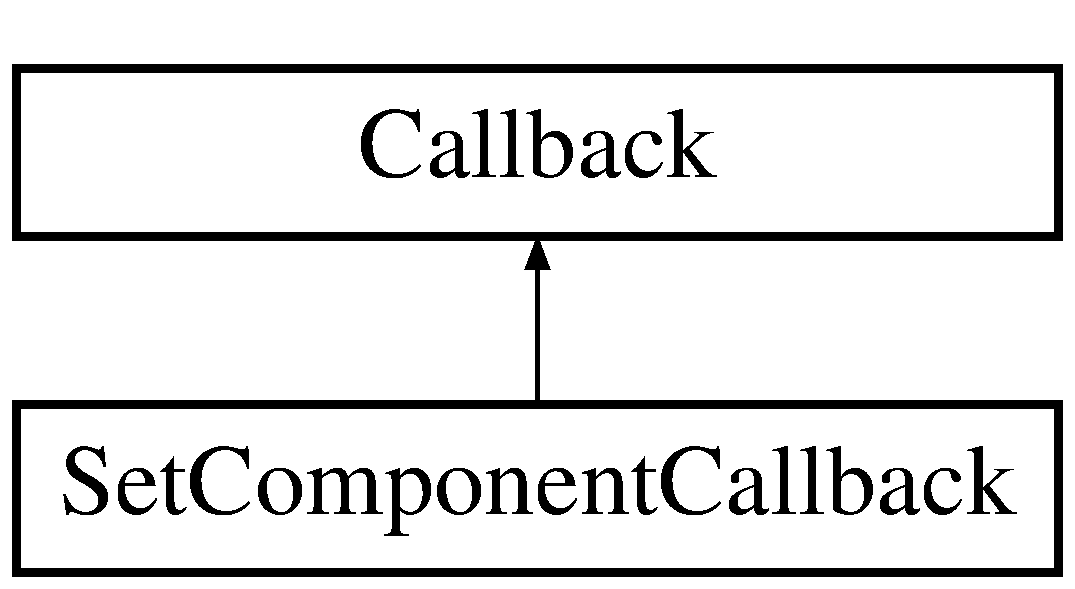
\includegraphics[height=2.000000cm]{structSetComponentCallback}
\end{center}
\end{figure}
\subsection*{Public Member Functions}
\begin{DoxyCompactItemize}
\item 
{\bfseries Set\+Component\+Callback} (int c)\label{structSetComponentCallback_a0f2ca8f3081e1a3af4720d59f56df9fe}

\item 
virtual void {\bfseries Visit} (Node $\ast$n)\label{structSetComponentCallback_afd8b047454f94a9fc1983969ab7976fe}

\end{DoxyCompactItemize}
\subsection*{Public Attributes}
\begin{DoxyCompactItemize}
\item 
int {\bfseries component}\label{structSetComponentCallback_a544be9719b2ae2aedccf4aed117a6799}

\end{DoxyCompactItemize}


The documentation for this struct was generated from the following file\+:\begin{DoxyCompactItemize}
\item 
Motion\+Planner.\+cpp\end{DoxyCompactItemize}

\section{Single\+Obstacle\+C\+Space Class Reference}
\label{classSingleObstacleCSpace}\index{Single\+Obstacle\+C\+Space@{Single\+Obstacle\+C\+Space}}


Converges an \doxyref{Explicit\+C\+Space}{p.}{classExplicitCSpace} to a regular \doxyref{C\+Space}{p.}{classCSpace} based on one selected obstacle.  




{\ttfamily \#include $<$Explicit\+C\+Space.\+h$>$}

Inheritance diagram for Single\+Obstacle\+C\+Space\+:\begin{figure}[H]
\begin{center}
\leavevmode
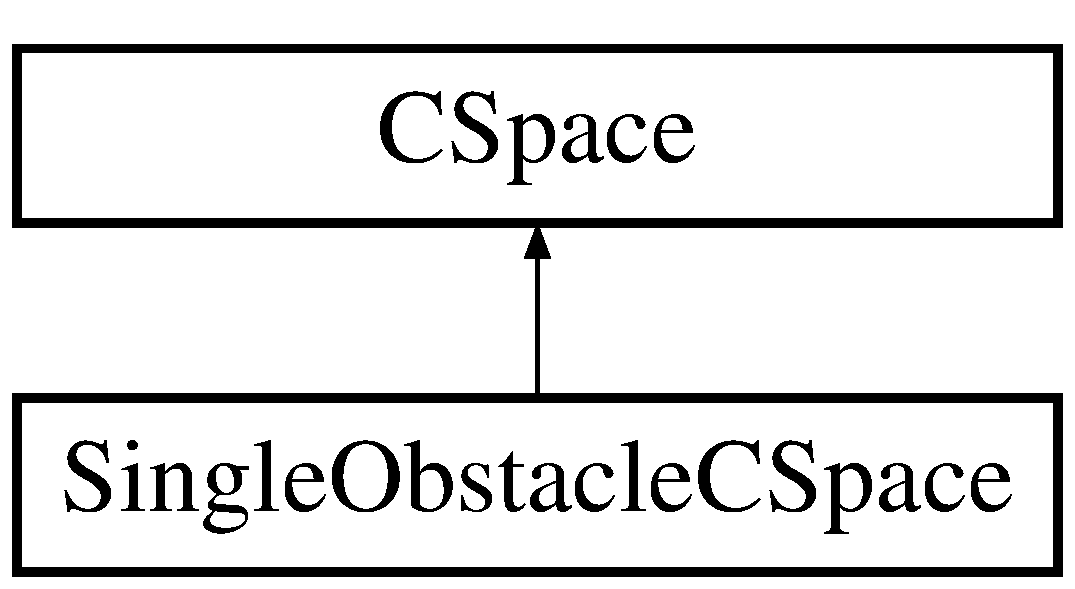
\includegraphics[height=2.000000cm]{classSingleObstacleCSpace}
\end{center}
\end{figure}
\subsection*{Public Member Functions}
\begin{DoxyCompactItemize}
\item 
{\bfseries Single\+Obstacle\+C\+Space} ({\bf Explicit\+C\+Space} $\ast$base\+Space, int obstacle)\label{classSingleObstacleCSpace_a7685a3cf6d8fca975314b2d2ee9162d4}

\item 
virtual bool {\bfseries Is\+Feasible} (const Config \&q)\label{classSingleObstacleCSpace_abf56f707f0030f9cb48082532eafb38c}

\item 
virtual {\bf Edge\+Planner} $\ast$ {\bfseries Local\+Planner} (const Config \&a, const Config \&b)\label{classSingleObstacleCSpace_adb1b4d2e9517f3e3f29019e7d36392b3}

\item 
virtual void {\bfseries Sample} (Config \&x)\label{classSingleObstacleCSpace_abe017ce5327656b119a526a88bea80a1}

\item 
virtual void {\bfseries Sample\+Neighborhood} (const Config \&c, double r, Config \&x)\label{classSingleObstacleCSpace_af97efa4198eee01044f0351b5205faae}

\item 
virtual double {\bf Distance} (const Config \&x, const Config \&y)\label{classSingleObstacleCSpace_aa66fd6cdcddbe8fece308ce13bb0a582}

\begin{DoxyCompactList}\small\item\em optionally overrideable (default uses euclidean space) \end{DoxyCompactList}\item 
virtual void {\bfseries Interpolate} (const Config \&x, const Config \&y, double u, Config \&out)\label{classSingleObstacleCSpace_a9361e0f3fff0bd54ae6ba7d3da81d422}

\end{DoxyCompactItemize}
\subsection*{Public Attributes}
\begin{DoxyCompactItemize}
\item 
{\bf Explicit\+C\+Space} $\ast$ {\bfseries base\+Space}\label{classSingleObstacleCSpace_a0f7f64d27ec08c09d46af530919a66bf}

\item 
int {\bfseries obstacle}\label{classSingleObstacleCSpace_a51cd1bb5b5ea66af8639f67c493b817b}

\end{DoxyCompactItemize}


\subsection{Detailed Description}
Converges an \doxyref{Explicit\+C\+Space}{p.}{classExplicitCSpace} to a regular \doxyref{C\+Space}{p.}{classCSpace} based on one selected obstacle. 

The documentation for this class was generated from the following files\+:\begin{DoxyCompactItemize}
\item 
Explicit\+C\+Space.\+h\item 
Explicit\+C\+Space.\+cpp\end{DoxyCompactItemize}

\section{Straight\+Line\+Epsilon\+Planner Class Reference}
\label{classStraightLineEpsilonPlanner}\index{Straight\+Line\+Epsilon\+Planner@{Straight\+Line\+Epsilon\+Planner}}


Straight-\/line edge planner that divides the segment until epsilon is reached.  




{\ttfamily \#include $<$Edge\+Planner.\+h$>$}

Inheritance diagram for Straight\+Line\+Epsilon\+Planner\+:\begin{figure}[H]
\begin{center}
\leavevmode
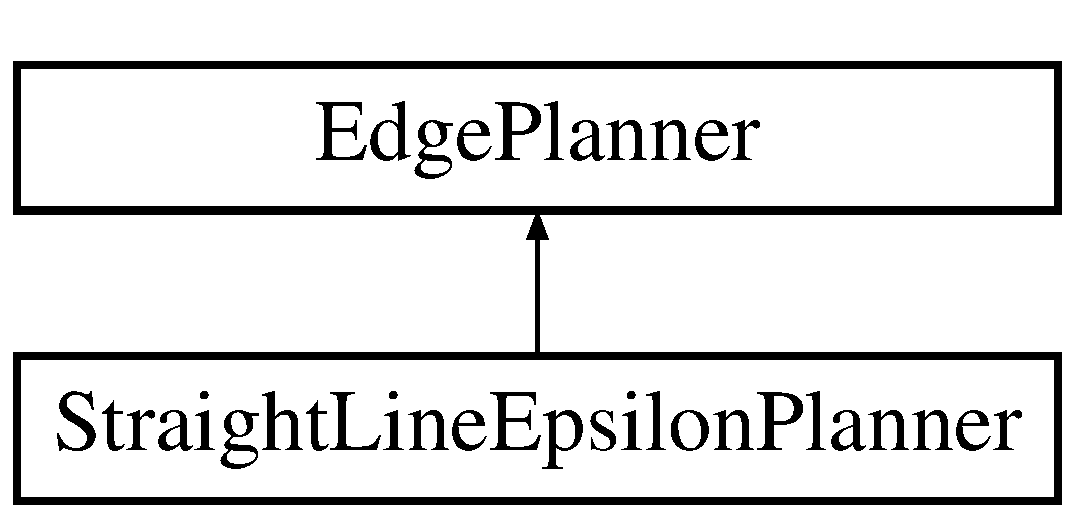
\includegraphics[height=2.000000cm]{classStraightLineEpsilonPlanner}
\end{center}
\end{figure}
\subsection*{Public Member Functions}
\begin{DoxyCompactItemize}
\item 
{\bfseries Straight\+Line\+Epsilon\+Planner} (const Config \&a, const Config \&b, {\bf C\+Space} $\ast$space, double epsilon)\label{classStraightLineEpsilonPlanner_ac641c0b7e08bba510366e6c9a5ad3cfb}

\item 
virtual bool {\bfseries Is\+Visible} ()\label{classStraightLineEpsilonPlanner_ae65de367b00380d4ac1b0b665bf3ec14}

\item 
virtual void {\bfseries Eval} (double u, Config \&x) const \label{classStraightLineEpsilonPlanner_acd8e8bbe6a515c94e63495f4c783ab20}

\item 
virtual const Config \& {\bfseries Start} () const \label{classStraightLineEpsilonPlanner_a35ad51c5701b7bbd22ec8cf0823fffa3}

\item 
virtual const Config \& {\bfseries Goal} () const \label{classStraightLineEpsilonPlanner_a36d9fd400faea7cc76924a97b61f2989}

\item 
virtual {\bf C\+Space} $\ast$ {\bfseries Space} () const \label{classStraightLineEpsilonPlanner_ad8151ca526cb6306df5cc4369820b81a}

\item 
virtual {\bf Edge\+Planner} $\ast$ {\bfseries Copy} () const \label{classStraightLineEpsilonPlanner_a297ae899e2a35268317bf3b49d74abde}

\item 
virtual {\bf Edge\+Planner} $\ast$ {\bfseries Reverse\+Copy} () const \label{classStraightLineEpsilonPlanner_ae1dd836c26ce2c8efdd37007563a37dd}

\item 
virtual double {\bfseries Priority} () const \label{classStraightLineEpsilonPlanner_afed110be4d704e15845a8f8b6534f320}

\item 
virtual bool {\bfseries Plan} ()\label{classStraightLineEpsilonPlanner_ac5ed85b1b379500fbf3e28e1cf10b0ed}

\item 
virtual bool {\bfseries Done} () const \label{classStraightLineEpsilonPlanner_a1edaa4b0182c5bd299bc298ea1fca986}

\item 
virtual bool {\bfseries Failed} () const \label{classStraightLineEpsilonPlanner_ac991b0a81c5fa084ded9291d03c8a4a4}

\end{DoxyCompactItemize}
\subsection*{Public Attributes}
\begin{DoxyCompactItemize}
\item 
Config {\bfseries a}\label{classStraightLineEpsilonPlanner_a283302b601941f0570e007e2ea601eb6}

\item 
Config {\bfseries b}\label{classStraightLineEpsilonPlanner_aa5b324ce8a64dfd718464cbd4cfc7f97}

\item 
{\bf C\+Space} $\ast$ {\bfseries space}\label{classStraightLineEpsilonPlanner_af53624bcda4e4449667b70142bde4dc5}

\item 
double {\bfseries epsilon}\label{classStraightLineEpsilonPlanner_a1d69f13d62136ef826b90847c9f2e243}

\end{DoxyCompactItemize}


\subsection{Detailed Description}
Straight-\/line edge planner that divides the segment until epsilon is reached. 

The documentation for this class was generated from the following files\+:\begin{DoxyCompactItemize}
\item 
Edge\+Planner.\+h\item 
Edge\+Planner.\+cpp\end{DoxyCompactItemize}

\section{Straight\+Line\+Obstacle\+Distance\+Planner Class Reference}
\label{classStraightLineObstacleDistancePlanner}\index{Straight\+Line\+Obstacle\+Distance\+Planner@{Straight\+Line\+Obstacle\+Distance\+Planner}}


Straight-\/line edge planner that divides the segment until the segment distance is below \doxyref{C\+Space.\+Obstacle\+Distance()}{p.}{classCSpace_a364b5b0ebcc258c39a263914ad3a0a89}  




{\ttfamily \#include $<$Edge\+Planner.\+h$>$}

Inheritance diagram for Straight\+Line\+Obstacle\+Distance\+Planner\+:\begin{figure}[H]
\begin{center}
\leavevmode
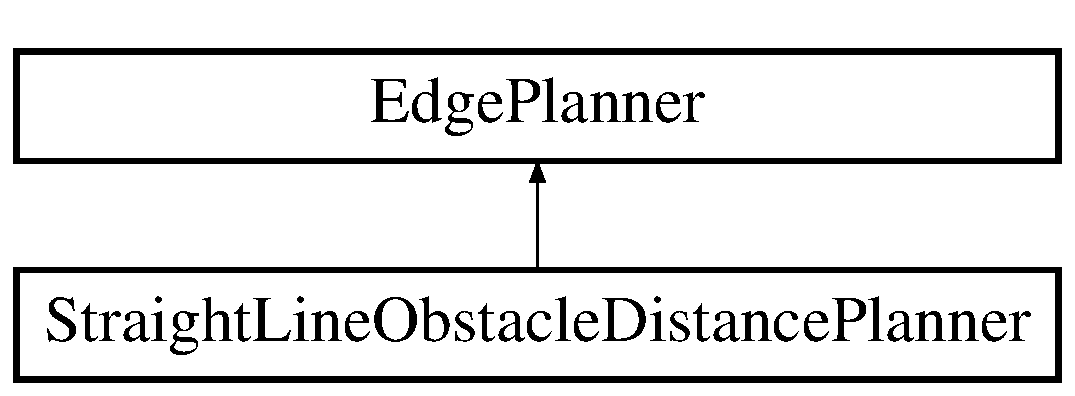
\includegraphics[height=2.000000cm]{classStraightLineObstacleDistancePlanner}
\end{center}
\end{figure}
\subsection*{Public Member Functions}
\begin{DoxyCompactItemize}
\item 
{\bfseries Straight\+Line\+Obstacle\+Distance\+Planner} (const Config \&a, const Config \&b, {\bf C\+Space} $\ast$space)\label{classStraightLineObstacleDistancePlanner_a0644aa15e66d750a77e484438c05b9cf}

\item 
virtual bool {\bfseries Is\+Visible} ()\label{classStraightLineObstacleDistancePlanner_ad09c3a05037f9060cfcc317beec45736}

\item 
virtual void {\bfseries Eval} (double u, Config \&x) const \label{classStraightLineObstacleDistancePlanner_a28b92e7fae2f95ff5bee9cc2b1fb9ebd}

\item 
virtual const Config \& {\bfseries Start} () const \label{classStraightLineObstacleDistancePlanner_a8de1c8630d826dce8a13fccf90dfa90a}

\item 
virtual const Config \& {\bfseries Goal} () const \label{classStraightLineObstacleDistancePlanner_a46a2246ea836ecc225dc303375791801}

\item 
virtual {\bf C\+Space} $\ast$ {\bfseries Space} () const \label{classStraightLineObstacleDistancePlanner_ab1da0d157cd71a019d35d96a51760135}

\item 
virtual {\bf Edge\+Planner} $\ast$ {\bfseries Copy} () const \label{classStraightLineObstacleDistancePlanner_a6337ab3766a3ce8d9c6df93ec18d62d0}

\item 
virtual {\bf Edge\+Planner} $\ast$ {\bfseries Reverse\+Copy} () const \label{classStraightLineObstacleDistancePlanner_a31a5950fa1b1e51a16f6f7376e5f7463}

\item 
bool {\bfseries Check\+Visibility} (const Config \&a, const Config \&b, double da, double db)\label{classStraightLineObstacleDistancePlanner_a8d31bf14300e7e8904d4023d69476d8e}

\end{DoxyCompactItemize}
\subsection*{Public Attributes}
\begin{DoxyCompactItemize}
\item 
Config {\bfseries a}\label{classStraightLineObstacleDistancePlanner_ac5ea07072ed4422427e6582884e424aa}

\item 
Config {\bfseries b}\label{classStraightLineObstacleDistancePlanner_afd8bc0a84dbb1d0b074e004179bd57ed}

\item 
{\bf C\+Space} $\ast$ {\bfseries space}\label{classStraightLineObstacleDistancePlanner_a42ed439f4ecc85365f43ef38d78ff714}

\end{DoxyCompactItemize}


\subsection{Detailed Description}
Straight-\/line edge planner that divides the segment until the segment distance is below \doxyref{C\+Space.\+Obstacle\+Distance()}{p.}{classCSpace_a364b5b0ebcc258c39a263914ad3a0a89} 

The documentation for this class was generated from the following files\+:\begin{DoxyCompactItemize}
\item 
Edge\+Planner.\+h\item 
Edge\+Planner.\+cpp\end{DoxyCompactItemize}

\section{Subgroup\+Explicit\+C\+Space Class Reference}
\label{classSubgroupExplicitCSpace}\index{Subgroup\+Explicit\+C\+Space@{Subgroup\+Explicit\+C\+Space}}


Groups together multiple obstacles from an \doxyref{Explicit\+C\+Space}{p.}{classExplicitCSpace}.  




{\ttfamily \#include $<$Explicit\+C\+Space.\+h$>$}

Inheritance diagram for Subgroup\+Explicit\+C\+Space\+:\begin{figure}[H]
\begin{center}
\leavevmode
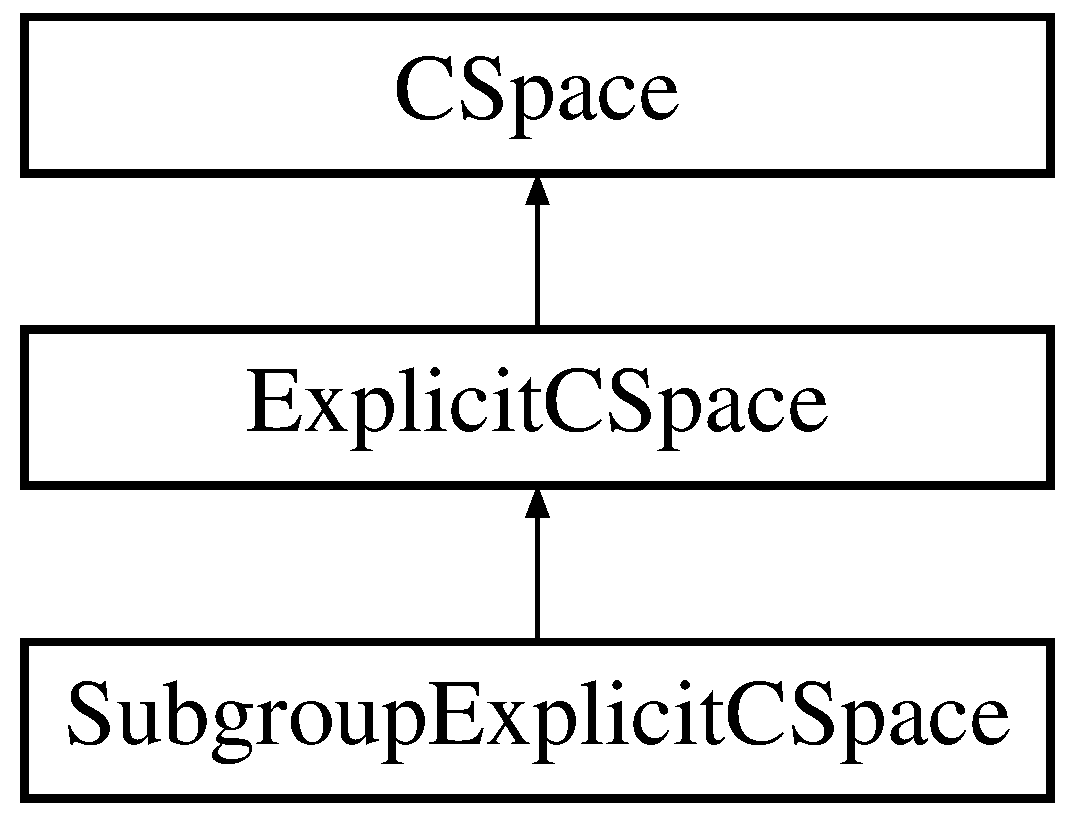
\includegraphics[height=3.000000cm]{classSubgroupExplicitCSpace}
\end{center}
\end{figure}
\subsection*{Public Member Functions}
\begin{DoxyCompactItemize}
\item 
{\bfseries Subgroup\+Explicit\+C\+Space} ({\bf Explicit\+C\+Space} $\ast$base\+Space)\label{classSubgroupExplicitCSpace_ac9d56ea52e49d82d4ab6d071e69f3e47}

\item 
void {\bfseries Ungroup} ()\label{classSubgroupExplicitCSpace_a9ac979d67effb2366d8309b871220de4}

\item 
void {\bfseries Group} (int i, int j)\label{classSubgroupExplicitCSpace_a31f72d26ed662eeae70317afc234f524}

\item 
virtual bool {\bf Is\+Feasible} (const Config \&, int obstacle)\label{classSubgroupExplicitCSpace_a4550de0947de8d0ad4a496422af659de}

\begin{DoxyCompactList}\small\item\em Implement this\+: single-\/obstacle feasibility check. \end{DoxyCompactList}\item 
virtual {\bf Edge\+Planner} $\ast$ {\bf Local\+Planner} (const Config \&a, const Config \&b)\label{classSubgroupExplicitCSpace_a0e313f00a5c123d54e8dcd3a06762ba0}

\begin{DoxyCompactList}\small\item\em Implement this (optional)\+: all obstacle local planner. \end{DoxyCompactList}\item 
virtual {\bf Edge\+Planner} $\ast$ {\bf Local\+Planner} (const Config \&a, const Config \&b, int obstacle)\label{classSubgroupExplicitCSpace_afb82f0fb666da7a091ee81a4c156785a}

\begin{DoxyCompactList}\small\item\em Implement this\+: single-\/obstacle local planner. \end{DoxyCompactList}\item 
virtual int {\bf Num\+Obstacles} ()\label{classSubgroupExplicitCSpace_af8b539a67a294af256ad05b7a7a44abe}

\begin{DoxyCompactList}\small\item\em Implement this\+: returns the number of obstacles. \end{DoxyCompactList}\item 
virtual std\+::string {\bf Obstacle\+Name} (int obstacle)\label{classSubgroupExplicitCSpace_ad45cb9cfbcced138256ad15108b62311}

\begin{DoxyCompactList}\small\item\em Implement this\+: returns the name of obstacle. \end{DoxyCompactList}\item 
virtual double {\bf Obstacle\+Distance} (const Config \&a, int obstacle)\label{classSubgroupExplicitCSpace_a459cc5f61c7fc4c2179ff278ac3aff35}

\begin{DoxyCompactList}\small\item\em Optional\+: for local planners using obstacle distance. \end{DoxyCompactList}\item 
virtual void {\bfseries Sample} (Config \&x)\label{classSubgroupExplicitCSpace_a49896bdaa737630c1644aa470d4171b7}

\item 
virtual void {\bfseries Sample\+Neighborhood} (const Config \&c, double r, Config \&x)\label{classSubgroupExplicitCSpace_a814c6460c9dc4aeb1cb08f59a2a1b14d}

\item 
virtual double {\bf Distance} (const Config \&x, const Config \&y)\label{classSubgroupExplicitCSpace_aa19a708cadc862d2ce5eac6611bd0558}

\begin{DoxyCompactList}\small\item\em optionally overrideable (default uses euclidean space) \end{DoxyCompactList}\item 
virtual void {\bfseries Interpolate} (const Config \&x, const Config \&y, double u, Config \&out)\label{classSubgroupExplicitCSpace_af2b628a0c95c04e2e91b748bdc27b518}

\end{DoxyCompactItemize}
\subsection*{Public Attributes}
\begin{DoxyCompactItemize}
\item 
{\bf Explicit\+C\+Space} $\ast$ {\bfseries base\+Space}\label{classSubgroupExplicitCSpace_a41381e04f4949194420d8967c27cbeba}

\item 
std\+::vector$<$ std\+::vector$<$ int $>$ $>$ {\bfseries groups}\label{classSubgroupExplicitCSpace_aa0ec0a8aa2ddd9aa4cc26d0aeb79f318}

\item 
std\+::vector$<$ std\+::string $>$ {\bfseries group\+Names}\label{classSubgroupExplicitCSpace_aa579937f512b522cdaca424bdf93a441}

\end{DoxyCompactItemize}


\subsection{Detailed Description}
Groups together multiple obstacles from an \doxyref{Explicit\+C\+Space}{p.}{classExplicitCSpace}. 

The documentation for this class was generated from the following files\+:\begin{DoxyCompactItemize}
\item 
Explicit\+C\+Space.\+h\item 
Explicit\+C\+Space.\+cpp\end{DoxyCompactItemize}

\section{Subset Struct Reference}
\label{structSubset}\index{Subset@{Subset}}
\subsection*{Public Member Functions}
\begin{DoxyCompactItemize}
\item 
{\bfseries Subset} (int max\+Item=0)\label{structSubset_a08f4b42ff7f42a3943224d0d003e6e03}

\item 
{\bfseries Subset} (const {\bf Subset} \&s)\label{structSubset_abf0b9dfab6abc093e2390994e6bcecb3}

\item 
{\bfseries Subset} (const std\+::vector$<$ bool $>$ \&bits)\label{structSubset_aabfc97f4b68c7dfc984b6488f6d5a75c}

\item 
bool {\bfseries operator$<$} (const {\bf Subset} \&s) const \label{structSubset_a4c8589928031aac9d25c29059db923a0}

\item 
bool {\bfseries operator$>$} (const {\bf Subset} \&s) const \label{structSubset_ad0b9406c15f4c0e7d1b7a8212d0fd7c4}

\item 
bool {\bfseries operator==} (const {\bf Subset} \&s) const \label{structSubset_aa80320c63aa36159e85c9cdb19faead3}

\item 
bool {\bfseries operator!=} (const {\bf Subset} \&s) const \label{structSubset_ad41068de94ff063c109f63048631b0cc}

\item 
{\bf Subset} {\bfseries operator+} (const {\bf Subset} \&s) const \label{structSubset_afab6bdecb3c4cc963283a89be5ee9283}

\item 
{\bf Subset} {\bfseries operator-\/} () const \label{structSubset_ad0bc4d41b2b1c4d5a89ed59822b371b0}

\item 
int {\bfseries count} () const \label{structSubset_aa4f1cce13bf3e80e7f2f4e79381270ea}

\item 
double {\bfseries cost} (const std\+::vector$<$ double $>$ \&weights) const \label{structSubset_aa4babe0611921ccf807030970f137803}

\item 
bool {\bfseries is\+\_\+subset} (const {\bf Subset} \&s) const \label{structSubset_ab87530f02b32c881885886f7d0b1bd54}

\end{DoxyCompactItemize}
\subsection*{Public Attributes}
\begin{DoxyCompactItemize}
\item 
int {\bfseries max\+Item}\label{structSubset_a32b8d5fac73f7d2da47786f862bbdf32}

\item 
std\+::set$<$ int $>$ {\bfseries items}\label{structSubset_a023b31e7ec433e56971e0fff91ded3cf}

\end{DoxyCompactItemize}


The documentation for this struct was generated from the following files\+:\begin{DoxyCompactItemize}
\item 
Explaining\+Planner.\+h\item 
Explaining\+Planner.\+cpp\end{DoxyCompactItemize}

\section{Subset\+Cost Struct Reference}
\label{structSubsetCost}\index{Subset\+Cost@{Subset\+Cost}}
\subsection*{Public Member Functions}
\begin{DoxyCompactItemize}
\item 
{\bfseries Subset\+Cost} (int max\+Item=0, double cost=0, vector$<$ double $>$ $\ast$\+\_\+weights=N\+U\+LL)\label{structSubsetCost_a5cd325a13426f6241c30e43e8abbbd7c}

\item 
{\bfseries Subset\+Cost} (const {\bf Subset} \&s, double cost=0, vector$<$ double $>$ $\ast$\+\_\+weights=N\+U\+LL)\label{structSubsetCost_af2a38a5b2d3ff85815549073c5a96c5d}

\item 
{\bfseries Subset\+Cost} (const {\bf Subset\+Cost} \&s)\label{structSubsetCost_afdad501aea359a73818fa7c4ca8dc730}

\item 
bool {\bfseries operator$<$} (const {\bf Subset\+Cost} \&s) const \label{structSubsetCost_aa8a97601359c65b13fca740e4c4e89b0}

\item 
bool {\bfseries operator$>$} (const {\bf Subset\+Cost} \&s) const \label{structSubsetCost_a06643beecbf5fd9e6b2c66c7b78e057f}

\item 
bool {\bfseries operator==} (const {\bf Subset\+Cost} \&s) const \label{structSubsetCost_adcc0d15e669cfa27156e6c92e3f48b7e}

\item 
bool {\bfseries operator!=} (const {\bf Subset\+Cost} \&s) const \label{structSubsetCost_aa13cfb493fa628c3efa475560ec4d0c5}

\item 
{\bf Subset\+Cost} {\bfseries operator+} (const {\bf Subset\+Cost} \&s) const \label{structSubsetCost_a4db9ca0682d964dc0ceec7f2c94cb6ca}

\item 
{\bf Subset\+Cost} {\bfseries operator-\/} () const \label{structSubsetCost_a050ecb7cb0a7ffed6bd362c80f572101}

\end{DoxyCompactItemize}
\subsection*{Public Attributes}
\begin{DoxyCompactItemize}
\item 
{\bf Subset} {\bfseries subset}\label{structSubsetCost_ada8f2862c99177610ea9ebfe808adf77}

\item 
double {\bfseries path\+Cost}\label{structSubsetCost_ac32716e4d65b0fef5ec655331accf647}

\item 
vector$<$ double $>$ $\ast$ {\bfseries weights}\label{structSubsetCost_a4ebbe1302eef83f7224ec12a8df40964}

\end{DoxyCompactItemize}


\subsection{Detailed Description}
Uses size comparisons for a partial ordering, rather than element comparisons 

The documentation for this struct was generated from the following file\+:\begin{DoxyCompactItemize}
\item 
Explaining\+Planner.\+cpp\end{DoxyCompactItemize}

\section{Subset\+Explicit\+C\+Space Class Reference}
\label{classSubsetExplicitCSpace}\index{Subset\+Explicit\+C\+Space@{Subset\+Explicit\+C\+Space}}


Extracts a subset of obstacles from an \doxyref{Explicit\+C\+Space}{p.}{classExplicitCSpace}.  




{\ttfamily \#include $<$Explicit\+C\+Space.\+h$>$}

Inheritance diagram for Subset\+Explicit\+C\+Space\+:\begin{figure}[H]
\begin{center}
\leavevmode
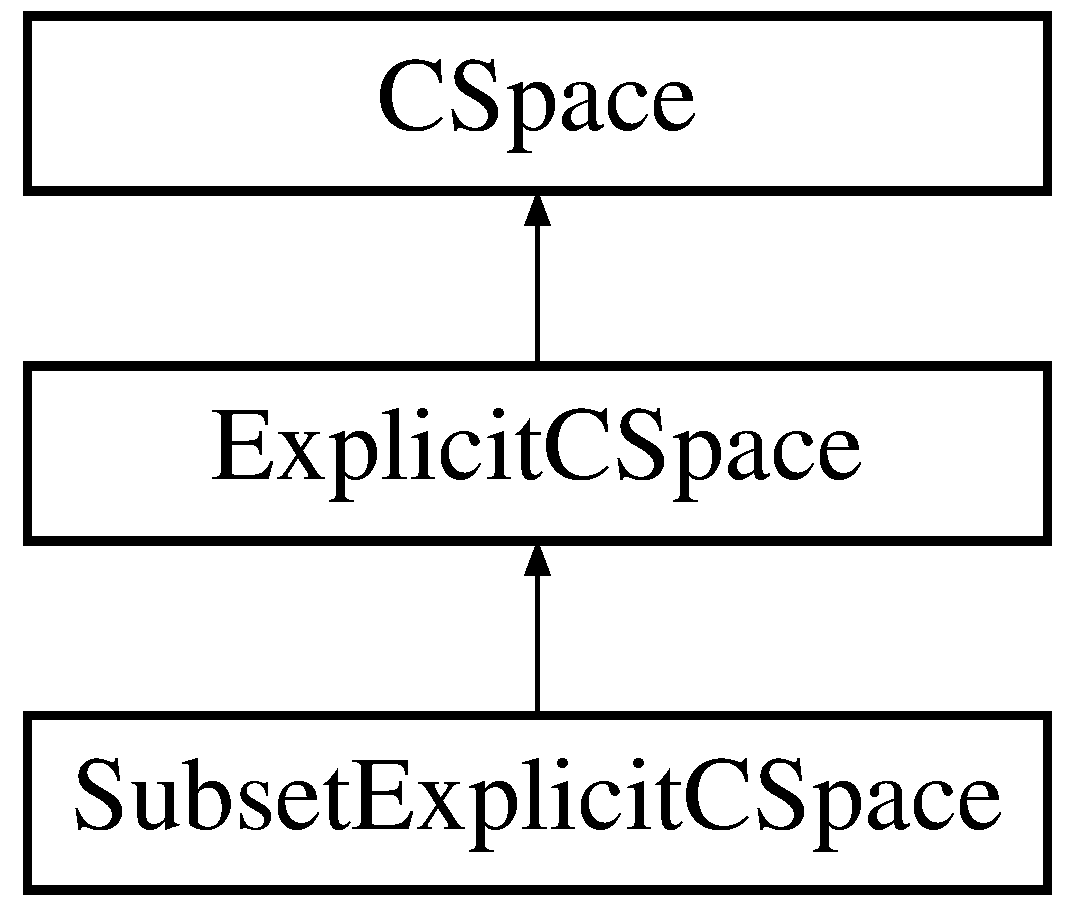
\includegraphics[height=3.000000cm]{classSubsetExplicitCSpace}
\end{center}
\end{figure}
\subsection*{Public Member Functions}
\begin{DoxyCompactItemize}
\item 
{\bfseries Subset\+Explicit\+C\+Space} ({\bf Explicit\+C\+Space} $\ast$base\+Space)\label{classSubsetExplicitCSpace_a1d6500746f092bced9ca8c08439adc0e}

\item 
{\bfseries Subset\+Explicit\+C\+Space} ({\bf Explicit\+C\+Space} $\ast$base\+Space, int obstacle)\label{classSubsetExplicitCSpace_a2bcd5da2d02b66e190885eb49f92dd39}

\item 
void {\bf Enable\+All} ()\label{classSubsetExplicitCSpace_af15f473eeadbba58f60d23cf9884e922}

\begin{DoxyCompactList}\small\item\em Turn on all constraints. \end{DoxyCompactList}\item 
void {\bf Enable\+None} ()\label{classSubsetExplicitCSpace_ae7aa34760cdc52f9a1a21c86f5a92f13}

\begin{DoxyCompactList}\small\item\em Turn off all constraints. \end{DoxyCompactList}\item 
virtual bool {\bf Is\+Feasible} (const Config \&, int obstacle)\label{classSubsetExplicitCSpace_a773a6d83691675466d07923bc82d14ad}

\begin{DoxyCompactList}\small\item\em Implement this\+: single-\/obstacle feasibility check. \end{DoxyCompactList}\item 
virtual {\bf Edge\+Planner} $\ast$ {\bf Local\+Planner} (const Config \&a, const Config \&b)\label{classSubsetExplicitCSpace_a99a68df6f72256d5f7a01de8a681a6b9}

\begin{DoxyCompactList}\small\item\em Implement this (optional)\+: all obstacle local planner. \end{DoxyCompactList}\item 
virtual {\bf Edge\+Planner} $\ast$ {\bf Local\+Planner} (const Config \&a, const Config \&b, int obstacle)\label{classSubsetExplicitCSpace_a00ba1b23d12b9bf27dc3aebf450a4cc7}

\begin{DoxyCompactList}\small\item\em Implement this\+: single-\/obstacle local planner. \end{DoxyCompactList}\item 
virtual int {\bf Num\+Obstacles} ()\label{classSubsetExplicitCSpace_ac3fd1ee0bdec0cfa4ac11af50402a9e7}

\begin{DoxyCompactList}\small\item\em Implement this\+: returns the number of obstacles. \end{DoxyCompactList}\item 
virtual std\+::string {\bf Obstacle\+Name} (int obstacle)\label{classSubsetExplicitCSpace_a41a2cdc371563e8eacc99633cf93bcff}

\begin{DoxyCompactList}\small\item\em Implement this\+: returns the name of obstacle. \end{DoxyCompactList}\item 
virtual double {\bf Obstacle\+Distance} (const Config \&a, int obstacle)\label{classSubsetExplicitCSpace_aa3f5f8f05dba341b271fd8e3fd658534}

\begin{DoxyCompactList}\small\item\em Optional\+: for local planners using obstacle distance. \end{DoxyCompactList}\item 
virtual void {\bfseries Sample} (Config \&x)\label{classSubsetExplicitCSpace_a1deddd28c38fa0ee57b203bff432f1de}

\item 
virtual void {\bfseries Sample\+Neighborhood} (const Config \&c, double r, Config \&x)\label{classSubsetExplicitCSpace_a94946b5d48b2bde4b0c9f04f00f0d1ce}

\item 
virtual double {\bf Distance} (const Config \&x, const Config \&y)\label{classSubsetExplicitCSpace_ac1a148c184aecec1276bee91657cd5a7}

\begin{DoxyCompactList}\small\item\em optionally overrideable (default uses euclidean space) \end{DoxyCompactList}\item 
virtual void {\bfseries Interpolate} (const Config \&x, const Config \&y, double u, Config \&out)\label{classSubsetExplicitCSpace_a0130ea98f0de04e60e7fb23be40af612}

\end{DoxyCompactItemize}
\subsection*{Public Attributes}
\begin{DoxyCompactItemize}
\item 
{\bf Explicit\+C\+Space} $\ast$ {\bfseries base\+Space}\label{classSubsetExplicitCSpace_adbc066ce0eab6e79ae1adbaa9c0b689e}

\item 
std\+::vector$<$ int $>$ {\bfseries active\+Subset}\label{classSubsetExplicitCSpace_a6e18e789f9a904f8186d63dddfab8fdc}

\end{DoxyCompactItemize}


\subsection{Detailed Description}
Extracts a subset of obstacles from an \doxyref{Explicit\+C\+Space}{p.}{classExplicitCSpace}. 

The documentation for this class was generated from the following files\+:\begin{DoxyCompactItemize}
\item 
Explicit\+C\+Space.\+h\item 
Explicit\+C\+Space.\+cpp\end{DoxyCompactItemize}

\section{Error\+Explaining\+Planner\+:\+:Transition Struct Reference}
\label{structErrorExplainingPlanner_1_1Transition}\index{Error\+Explaining\+Planner\+::\+Transition@{Error\+Explaining\+Planner\+::\+Transition}}
\subsection*{Public Attributes}
\begin{DoxyCompactItemize}
\item 
std\+::vector$<$ std\+::pair$<$ int, int $>$ $>$ {\bfseries connections}\label{structErrorExplainingPlanner_1_1Transition_aab8932432015b9aa75b703234dbfd059}

\end{DoxyCompactItemize}


The documentation for this struct was generated from the following file\+:\begin{DoxyCompactItemize}
\item 
Explaining\+Planner.\+h\end{DoxyCompactItemize}

\section{Multi\+Modal\+P\+RM\+:\+:Transition\+Index Struct Reference}
\label{structMultiModalPRM_1_1TransitionIndex}\index{Multi\+Modal\+P\+R\+M\+::\+Transition\+Index@{Multi\+Modal\+P\+R\+M\+::\+Transition\+Index}}
\subsection*{Public Member Functions}
\begin{DoxyCompactItemize}
\item 
bool {\bfseries operator$<$} (const {\bf Transition\+Index} \&t) const \label{structMultiModalPRM_1_1TransitionIndex_aa4ed901b786c7946500ce3f173c7ac07}

\end{DoxyCompactItemize}
\subsection*{Public Attributes}
\begin{DoxyCompactItemize}
\item 
int {\bfseries m1}\label{structMultiModalPRM_1_1TransitionIndex_a73f1ab9308d7ce35202f1980e9c72a0a}

\item 
int {\bfseries m2}\label{structMultiModalPRM_1_1TransitionIndex_a40b64be69191129772a1660a8caa419d}

\item 
int {\bfseries count}\label{structMultiModalPRM_1_1TransitionIndex_a191f1df07cce02ad6127bc8423b4a881}

\end{DoxyCompactItemize}


The documentation for this struct was generated from the following file\+:\begin{DoxyCompactItemize}
\item 
Multi\+Modal\+Planner.\+h\end{DoxyCompactItemize}

\section{Multi\+Modal\+P\+RM\+:\+:Transition\+Info Struct Reference}
\label{structMultiModalPRM_1_1TransitionInfo}\index{Multi\+Modal\+P\+R\+M\+::\+Transition\+Info@{Multi\+Modal\+P\+R\+M\+::\+Transition\+Info}}
\subsection*{Public Attributes}
\begin{DoxyCompactItemize}
\item 
int {\bfseries sample\+Count}\label{structMultiModalPRM_1_1TransitionInfo_a064d83eb1b966f212bd3f128cb391bd9}

\item 
vector$<$ Config $>$ {\bfseries transitions}\label{structMultiModalPRM_1_1TransitionInfo_ab2619d3c1da4076996151bea3a5b9070}

\item 
vector$<$ int $>$ {\bfseries prev\+Roadmap\+Indices}\label{structMultiModalPRM_1_1TransitionInfo_a98fe9675c4d7d21ccfdde938e24bbe7d}

\item 
vector$<$ int $>$ {\bfseries next\+Roadmap\+Indices}\label{structMultiModalPRM_1_1TransitionInfo_a6f86bbe21272da88c4f583054173a0d9}

\end{DoxyCompactItemize}


The documentation for this struct was generated from the following file\+:\begin{DoxyCompactItemize}
\item 
Multi\+Modal\+Planner.\+h\end{DoxyCompactItemize}

\section{Tree\+Roadmap\+Planner Class Reference}
\label{classTreeRoadmapPlanner}\index{Tree\+Roadmap\+Planner@{Tree\+Roadmap\+Planner}}


A base class to be used for tree-\/based roadmap planners.  




{\ttfamily \#include $<$Motion\+Planner.\+h$>$}

Inheritance diagram for Tree\+Roadmap\+Planner\+:\begin{figure}[H]
\begin{center}
\leavevmode
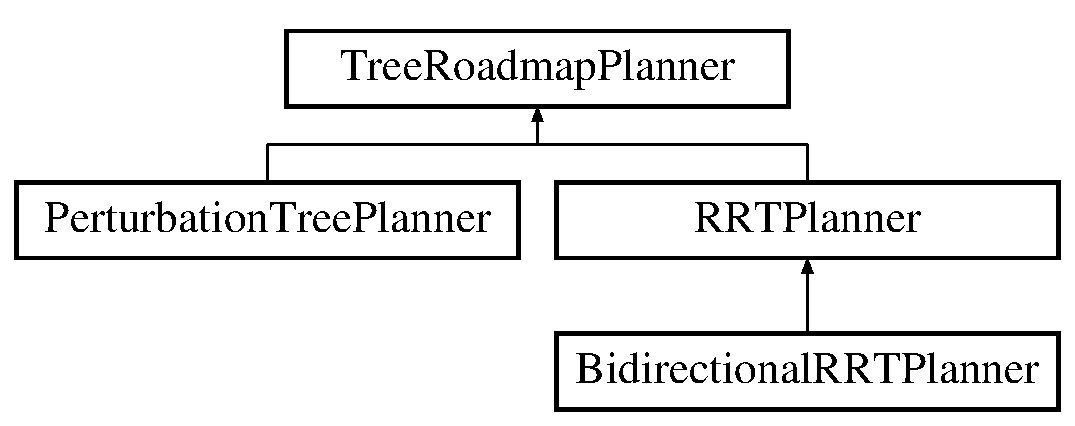
\includegraphics[height=3.000000cm]{classTreeRoadmapPlanner}
\end{center}
\end{figure}
\subsection*{Classes}
\begin{DoxyCompactItemize}
\item 
struct {\bf Milestone}
\end{DoxyCompactItemize}
\subsection*{Public Types}
\begin{DoxyCompactItemize}
\item 
typedef Graph\+::\+Tree\+Node$<$ {\bf Milestone}, Smart\+Pointer$<$ {\bf Edge\+Planner} $>$ $>$ {\bfseries Node}\label{classTreeRoadmapPlanner_a15e4ae956786e808f8fba50959ebf6cd}

\end{DoxyCompactItemize}
\subsection*{Public Member Functions}
\begin{DoxyCompactItemize}
\item 
{\bfseries Tree\+Roadmap\+Planner} ({\bf C\+Space} $\ast$)\label{classTreeRoadmapPlanner_a4a224cbd46b967627bf79020a8689ac1}

\item 
virtual void {\bfseries Generate\+Config} (Config \&x)\label{classTreeRoadmapPlanner_a0faebeade2d119af8cde3043283d375c}

\item 
virtual Node $\ast$ {\bfseries Add\+Milestone} (const Config \&x)\label{classTreeRoadmapPlanner_a7109b4f5ccba01f740a7f0e6ee8e3649}

\item 
virtual Node $\ast$ {\bfseries Add\+Feasible\+Milestone} (const Config \&x)\label{classTreeRoadmapPlanner_a8fa85aa4a97d7737a907870def10b767}

\item 
virtual Node $\ast$ {\bfseries Add\+Infeasible\+Milestone} (const Config \&x)\label{classTreeRoadmapPlanner_a25261ff00047ff40a9c80f74e2d877e7}

\item 
virtual Node $\ast$ {\bfseries Extend} ()\label{classTreeRoadmapPlanner_ad9c3c6d1d0767096a966ea3dac8bbbac}

\item 
virtual void {\bfseries Cleanup} ()\label{classTreeRoadmapPlanner_af3d85fd871852d0f5f0c08ff33d23f9c}

\item 
virtual void {\bfseries Connect\+To\+Neighbors} (Node $\ast$)\label{classTreeRoadmapPlanner_ade53159d1bd7e9625e55c723eeb74a5e}

\item 
virtual {\bf Edge\+Planner} $\ast$ {\bfseries Try\+Connect} (Node $\ast$, Node $\ast$)\label{classTreeRoadmapPlanner_a2d751322db677629e241652c54354bfa}

\item 
virtual Node $\ast$ {\bfseries Closest\+Milestone} (const Config \&x)\label{classTreeRoadmapPlanner_a674d861ad4b93a79ee78cb89fb45cf64}

\item 
virtual Node $\ast$ {\bfseries Closest\+Milestone\+In\+Component} (int component, const Config \&x)\label{classTreeRoadmapPlanner_a423c21dd97c0ef8bd3f63f18e1e65ab0}

\item 
virtual Node $\ast$ {\bfseries Closest\+Milestone\+In\+Subtree} (Node $\ast$node, const Config \&x)\label{classTreeRoadmapPlanner_a0bd96cb7b494dcb7ec59d88d43afcd49}

\item 
Node $\ast$ {\bfseries Try\+Extend} (Node $\ast$n, const Config \&x)\label{classTreeRoadmapPlanner_a1c400fc81cf394c6c4064aae09c64726}

\item 
void {\bfseries Attach\+Child} (Node $\ast$p, Node $\ast$c, {\bf Edge\+Planner} $\ast$e)\label{classTreeRoadmapPlanner_a81b930e7911f3854e86af44614a2cc43}

\item 
void {\bfseries Create\+Path} (Node $\ast$a, Node $\ast$b, {\bf Milestone\+Path} \&path)\label{classTreeRoadmapPlanner_a13204609fccf6991d0185a44a78669fe}

\end{DoxyCompactItemize}
\subsection*{Public Attributes}
\begin{DoxyCompactItemize}
\item 
{\bf C\+Space} $\ast$ {\bfseries space}\label{classTreeRoadmapPlanner_ac52ea753c027983d2240063878087a12}

\item 
std\+::vector$<$ Node $\ast$ $>$ {\bfseries connected\+Components}\label{classTreeRoadmapPlanner_af2e35ac540027c714769f6d43029d3f0}

\item 
double {\bfseries connection\+Threshold}\label{classTreeRoadmapPlanner_affbc62cb9c116b1a8553ae0145a18151}

\item 
std\+::vector$<$ Node $\ast$ $>$ {\bfseries milestones}\label{classTreeRoadmapPlanner_a6422c51272728af9ee68a77378489415}

\item 
Config {\bfseries x}\label{classTreeRoadmapPlanner_a2fe75f4a282c83c50592d5302b7296a8}

\end{DoxyCompactItemize}


\subsection{Detailed Description}
A base class to be used for tree-\/based roadmap planners. 

connection\+Threshold is the minimum distance two nodes must be before a connection may be made between them. This is infinity by default. If it is infinity, connections are attempted to the closest node in a different component. 

The documentation for this class was generated from the following files\+:\begin{DoxyCompactItemize}
\item 
Motion\+Planner.\+h\item 
Motion\+Planner.\+cpp\end{DoxyCompactItemize}

\section{True\+Edge\+Planner Class Reference}
\label{classTrueEdgePlanner}\index{True\+Edge\+Planner@{True\+Edge\+Planner}}


Edge planner that always is visible.  




{\ttfamily \#include $<$Edge\+Planner.\+h$>$}

Inheritance diagram for True\+Edge\+Planner\+:\begin{figure}[H]
\begin{center}
\leavevmode
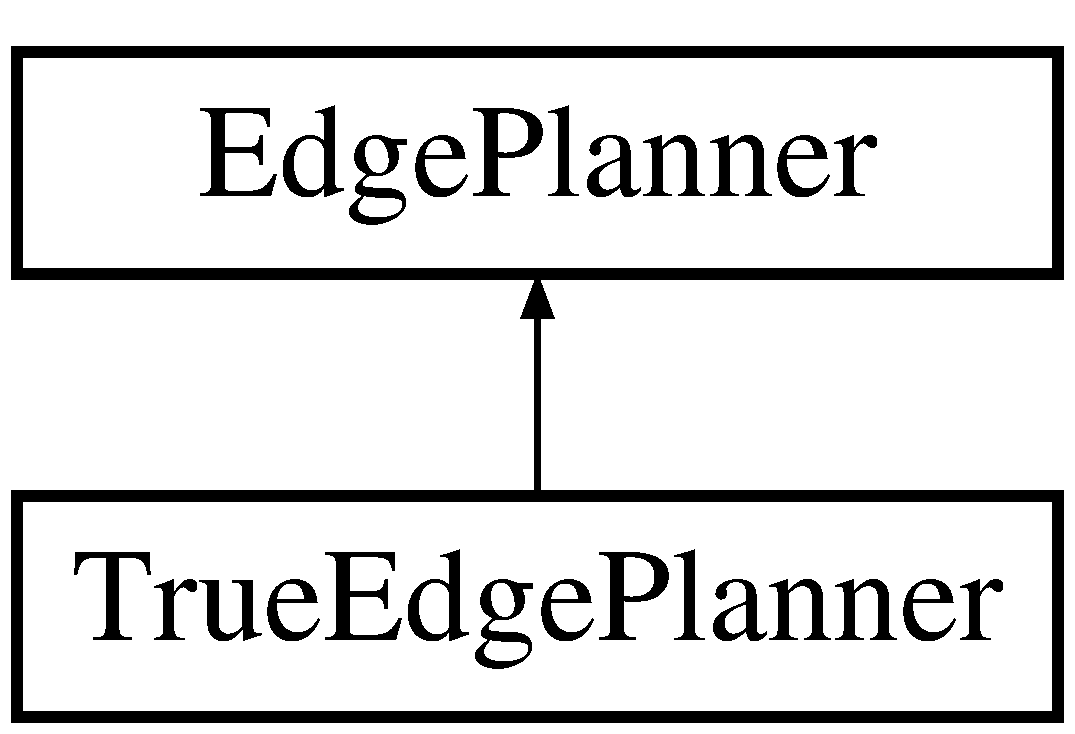
\includegraphics[height=2.000000cm]{classTrueEdgePlanner}
\end{center}
\end{figure}
\subsection*{Public Member Functions}
\begin{DoxyCompactItemize}
\item 
{\bfseries True\+Edge\+Planner} ({\bf C\+Space} $\ast$space, const Config \&x, const Config \&y)\label{classTrueEdgePlanner_a2fd99e4124f4705fdca92b9ce0c0749b}

\item 
virtual bool {\bfseries Is\+Visible} ()\label{classTrueEdgePlanner_afd8dfdcf8840ed1b833922afa72c63cb}

\item 
virtual void {\bfseries Eval} (double u, Config \&x) const \label{classTrueEdgePlanner_ae06917b8ec61ed6794952e587dd4bef8}

\item 
virtual const Config \& {\bfseries Start} () const \label{classTrueEdgePlanner_a63b03c66a70d3f7a6f86d6960c7cd749}

\item 
virtual const Config \& {\bfseries Goal} () const \label{classTrueEdgePlanner_a4d00b99c03fbddfe6d91d9bcdea466d0}

\item 
virtual {\bf C\+Space} $\ast$ {\bfseries Space} () const \label{classTrueEdgePlanner_a9be1ed91f63f887e6c9d6a595af65a96}

\item 
virtual {\bf Edge\+Planner} $\ast$ {\bfseries Copy} () const \label{classTrueEdgePlanner_ae21d6d22beab7e1eba87d928c0da0258}

\item 
virtual {\bf Edge\+Planner} $\ast$ {\bfseries Reverse\+Copy} () const \label{classTrueEdgePlanner_a650f6093c6a32595ad65115959a1d125}

\end{DoxyCompactItemize}
\subsection*{Public Attributes}
\begin{DoxyCompactItemize}
\item 
Config {\bfseries a}\label{classTrueEdgePlanner_a67ad4fda81bf524be1e6ec195603ecbc}

\item 
Config {\bfseries b}\label{classTrueEdgePlanner_a0e46198c3ebefbbc111a3bec99973f7d}

\item 
{\bf C\+Space} $\ast$ {\bfseries space}\label{classTrueEdgePlanner_a81296d34561ee07285a98a28abbc0cbe}

\end{DoxyCompactItemize}


\subsection{Detailed Description}
Edge planner that always is visible. 

The documentation for this class was generated from the following files\+:\begin{DoxyCompactItemize}
\item 
Edge\+Planner.\+h\item 
Edge\+Planner.\+cpp\end{DoxyCompactItemize}

\section{Update\+Priority\+S\+PP Struct Reference}
\label{structUpdatePrioritySPP}\index{Update\+Priority\+S\+PP@{Update\+Priority\+S\+PP}}
Inheritance diagram for Update\+Priority\+S\+PP\+:\begin{figure}[H]
\begin{center}
\leavevmode
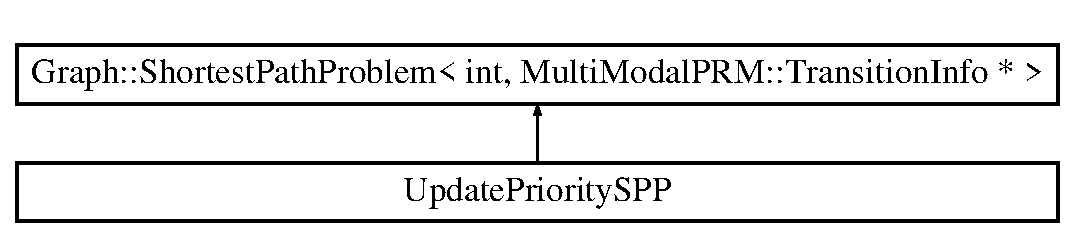
\includegraphics[height=2.000000cm]{structUpdatePrioritySPP}
\end{center}
\end{figure}
\subsection*{Public Member Functions}
\begin{DoxyCompactItemize}
\item 
{\bfseries Update\+Priority\+S\+PP} ({\bf Incremental\+M\+M\+P\+R\+M\+\_\+\+Search} \&\+\_\+g)\label{structUpdatePrioritySPP_a93902df43c81f2159b8b4077ae89efb0}

\item 
virtual void {\bfseries On\+Distance\+Update} (int n)\label{structUpdatePrioritySPP_af3a443286298411d71062659fcff3d9c}

\end{DoxyCompactItemize}
\subsection*{Public Attributes}
\begin{DoxyCompactItemize}
\item 
{\bf Incremental\+M\+M\+P\+R\+M\+\_\+\+Search} \& {\bfseries g}\label{structUpdatePrioritySPP_ac9a1c7978da69524185384168d5e2fee}

\end{DoxyCompactItemize}


The documentation for this struct was generated from the following files\+:\begin{DoxyCompactItemize}
\item 
Multi\+Modal\+Planner.\+h\item 
Multi\+Modal\+Planner.\+cpp\end{DoxyCompactItemize}

%--- End generated contents ---

% Index
\backmatter
\newpage
\phantomsection
\clearemptydoublepage
\addcontentsline{toc}{chapter}{Index}
\printindex

\end{document}
